松一又气吧,这将是全书最后一章,也是最简单的一章!

但这章的内容就是关于虚幻引擎中提供的基于距离场的全局光照技术吗? 你可以这么说,但是如果阅读完本章,你会发现这一章会包含一些比较综合性 的内容。严格来讲,虚幻引擎中的距离场并不是一种完整的全局光照技术,因 为它只提供可见性计算,并不包含表面着色的部分。那么为什么本书要将其单 独列作一章呢?

首先来讲,本书写作最初的动力和灵感其实来源于这一章的内容,这一章 也是本书最开始写作的起点。那个时候我开始学习虚幻引擎的一些知识,对于 渲染部分,其中的光照贴图,阴影贴图,预计算光照,环境立方体贴图,间接光 照缓存等,在概念上与其它引擎如 Unity3D 并没有太大差别,唯独关于距离场 的部分是其特有的特性。当我开始去学习这方面的知识时,我发现它还涉及很 多需要了解的预备知识或概念,例如关于表面的隐式表述,及其隐式表述表面 的渲染,光线步进,球体追踪等,另一方面,通过学习这些基础知识,我又发现 距离场的表述不仅能够用来实现可见性计算,它其实还包含其它一些应用,例如字体的渲染,表面的移位映射等。通过这些延伸学习,我不仅更好地理解了虚 幻引擎的距离场相关的概念和运用,而且建立起了一些关于表面表述等一些概 念更系统的知识图谱。这种学习思路很深刻地影响了这本书的写作风格,对于 本书中介绍的每一种全局光照技术,我的目标不是仅仅去介绍这种技术的算法 过程,而是通过这个技术概念为中心和起点,去延伸这种技术背后所涉及的所 有相关知识,这些相关知识可能是某个数学或物理方面的概念或方法,或者是 涉及其它一些技术。其它书的写作风格可能是以算法过程为核心,然后简要介 绍这些相关技术,甚至可能只给出参考文献让读者自行深入学习,而本书的写 作思路恰好相反,你最后会发现每个全局光照技术算法本身只是一个线索,我 们的重心放到了深入而详细地讨论这些相关技术上,而算法本身反而变得相对 次要。因为我认为,当读者深刻掌握了这些相关概念和知识,他/她才能更好地 理解这种技术本身,并且与此同时,我们建立起了一个更大更系统的知识图谱, 这就是本书前严中提到的知识逻辑性的概念。我们学习技术的目的不光是为了 解决工程问题,我们还需要用知识来丰富我们的大脑和精神世界。

另一方面,本书整本书的内容主要都是聚焦于光照传输(light transport), 我们还忽略了很多其它知识,例如关于表面表述更一般的概念,甚至前面还没 有很正式地介绍过如阴影贴图等概念,当然渲染的知识非常宽泛,我们不能指 望一本书能够涵盖所有内容,每本书有不同的偏重点。不过本章还是试图去尽 可能地去讨论一些更综合性的相关概念,同时本章将重心仅仅聚焦于一个可见 性计算,读者可以看到可见性在实时渲染中的重要性,以及为什么虚幻引擎会 单独仅为可见性计算耗费这么大的精力开发一种全新的技术。

好了,让我们开始阅读这最后的篇章,并提前恭喜你终于阅读完了全书吧!



\section{基础知识}
距离场本书并不是一种用于解决某个特定问题的技术或算法,它只是关于 物体表面的一种不同的表述,我们必须开发其它的算法使用距离场来解决一个 特定问题,本章我们将会看到距离场的几种不同的运用。当然距离场的运用非 常广泛\cite{a:3d-distance-fields-a-survey},本章我们仅聚焦于渲染方面的运用。

距离场(distance field)\myindex{距离场}{distance field}的概念来源于隐式表面表述,所以本节我们首先来 解释隐式函数怎样能够被用于表面表述,并介绍使用一个有符号距离函数来指 示物体表面的内部和外部,这种有符号的距离函数就是一种隐式表述,它形成 了一个距离场。

一个物体的表面可以被使用隐式函数隐式地表述,或者使用参数函数(parametric function)\myindex{参数函数}{parametric function}显式地表述(实际上在 \cite{b:AnIntegratedIntroductiontoCG}中一共有四种\footnote{另外两种是形变表面(deformed surfaces)\myindex{形变表面}{deformed surfaces}和程序化表面(procedural surfaces)\myindex{程序化表面}{procedural surfaces},形变表 面是指通过对其它表面执行变形操作而来,而程序化表面是指任意其它通过程序生成而不是 一个公式的形式表述的表面,例如分形(fractals)\myindex{分形}{fractals}。}标准 的方法用于表述表面)。为了渲染整个场景,这些函数可以被用于计算表面的法 线,以及执行渲染方程需要的光线-表面相交计算。

不同的表面表述往往需要使用不同的方法来渲染整个场景,这些往往都具 有各自的优缺点,本节我们简要介绍显式和隐式表面表述相关的概念,下一节 则会讨论常用的对隐式表面执行渲染的方法。



\subsection{参数化的表面}\label{sec:df-parametric-surface}
一个参数化表面(parametric surface)\myindex{参数化表面}{parametric surface}是指一个使用参数方程(parametric equation)\myindex{参数方程}{parametric equation}表述的表面,即是说对于表面上的每一个点 $P$,我们可以分配一对 参数值 $s,t$ 并使得可以用公式 $P = P(s,t)$ 来计算表面上的每一个点。例如对 于一个单位圆,它可以使用参数方程的形式表述为:

\begin{equation}
	\begin{aligned}
		x(\theta)=&\sin \theta\\
		y(\theta)=&\cos \theta
	\end{aligned}
\end{equation}

\noindent 这可以很容易通过下式得到验证:

\begin{equation}
	x^{2}(\theta)+y^{2}(\theta)-1=0
\end{equation}

通过使用参数化的表述,其表述的数据必须要包含表面上的每一个点,这 对于一个基本的表面是很简单的,例如平面,球面,圆柱面,圆环面等,但是它 很难描述一些复杂的表面,例如一个角色或者一座神庙。因此在计算机图形学 中,我们通常使用一个三角形来表述一个很小的表面块,成千上万的这种小三 角形就构成了一个模型的网格,我们记录下三角形每个顶点的位置,这些顶点 之间的点的位置则在渲染过程中的光栅化阶段被插值计算出来,如图\ref{f:df-rasterization}所示。

\begin{figure}
	\sidecaption
	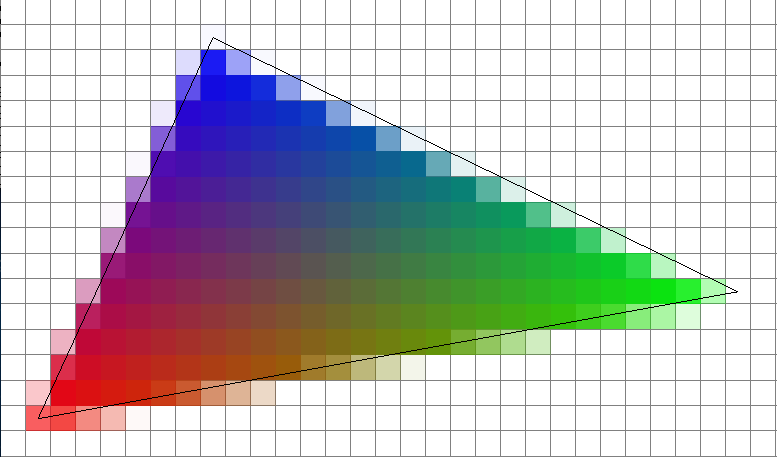
\includegraphics[width=0.65\textwidth]{figures/df/rasterization}
	\caption{使用光栅化,一个参数化的表面只需要记 录其中很少的一些顶点的位 置,即图中三角形的三个顶 点,更多的顶点则可以通过 图形硬件的插值特性计算出 来。}
	\label{f:df-rasterization}
\end{figure}

参数化表面是很容易生成的,但是要决定一个点 $P$ 是否位于一个参数化表 面却不那么简单,因为可能很难判定是否存在一个参数 $\theta$ 使得 $P = P (\theta)$。

所以这就是为什么光栅化很流行的原因,因为它不需要执行光线与表面的 相交计算,而只需要对表面上的所有点遍历一次并计算该点的颜色值,这通过 在图形管线中使用一个像素着色器计算渲染方程而得出。这种光照也称为局部 光照(local illumination)\myindex{局部光照}{local illumination},因为它仅仅考虑直接光照的反射。

但是在真实世界中,间接光照甚至是更加重要的,缺乏间接光照,则那些不 能直接被光源照射的区域将完全不可见,因此其渲染结果显然没有说服力。所 以人们提出了一些辅助方法用于在光栅化管线下模拟这些间接光照效果,例如 环境光照,天空盒光照等,这些光照可以被预计算并存储在一个纹理中,然后 在渲染时可以被映射到物体表面上。这意味着,我们不需要执行相交计算。

然而不幸的是,我们仍然需要去考虑点之间的相交判定,因为当一个物体 被动态移动时,这些预计算的贴图就不能再被使用。而真实世界却是一直都在 发生这样的改变的,例如角色几乎始终处于移动状态,天空的光照随时间在发 生变化,树上的叶子随时都在风中摇曳。这些变化导致光照和阴影都在时时刻 刻发生改变。

在一个场景中,通常只有少数物体是完全动态的,例如角色和车辆,许多 游戏引擎会对物体提供一个移动性属性,如图\ref{f:df-mobility}所示,所以动态的实时计算 可以只作用于这些少量动态物体上,所有固定和静态的物体都可以获得一定程 度上的预计算。然而对于那些少量的动态物体,它们的一些光照效果必须被实 时地计算,例如来自天空盒光照的环境遮挡,在 Unreal Engine 4 中他们提供表 面的另外一种表述来处理某些动态计算,而这种表述需要使用隐式表面表述。

\begin{figure}
\begin{fullwidth}
	\begin{subfigure}[b]{0.49\thewidth}
		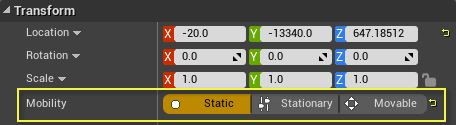
\includegraphics[width=\textwidth]{figures/df/IL_mobility}
		\caption{Light Mobility}
	\end{subfigure}
	\begin{subfigure}[b]{0.51\thewidth}
		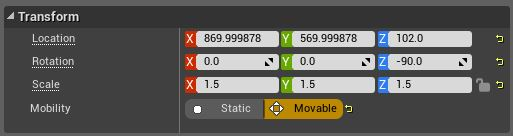
\includegraphics[width=\textwidth]{figures/df/TransformMobility}
		\caption{Actor Mobility}
	\end{subfigure}
	\caption{在 Unreal Engine 4 中,每个光源和角色都有一个移动性(mobility)属性, 所以引擎能够决定哪些光照和阴影的计算能够被预处理(图片来自 Unreal Engine 4 官方文档)}
	\label{f:df-mobility}
\end{fullwidth}
\end{figure}



\subsection{隐式表面}
光栅化不具备测试任意光线与表面是否相交的能力,而这种相交测试不仅 是为了计算间接光照,动态物体的某些直接光照效果(例如环境遮挡)也是需 要执行这种相交测试,因为这无法通过光栅化解决。所以我们引入隐式表面表 述的目标就是为了解决这种光线与表面的相交测试计算,这种表述作为传统的 三角形网格化表述的补充,就能够更高效地执行整个渲染计算。

一个隐式表面(implicit surface)\myindex{隐式表面}{implicit surface}是一些点 $P$ 的集合,其中所有这些点满 足一个隐式方程 $F(P) = 0$。基本上,函数 $F$ 是一个关于所有点 $P$ 的坐标值 $x,y$ 的多项式,例如对于一个单位圆,其隐式方程可以表述为:

\begin{equation}
	F(x,y)\equiv x^{2}+y^{2}=0
\end{equation}

这里定义 $\Omega^{−} = \{\vec{x}\mid|\vec{x}| < 1\}$ 为定义域中圆的内部,而 $\Omega^{+} = \{\vec{x}\mid|\vec{x}| > 1\}$ 为 定义域中圆的外部,内部和外部相交的边界就构成了这个圆 $\partial\Omega= \{\vec{x}\mid|\vec{x}| = 1\}$, 我们称这个边界为交界面\footnote{这里符号$\partial$表示边界,$\partial M$表示$M$的边界,例如:$\partial\{x:|x|≤2\}=\{x:|x|=2\}$。}(interface)\myindex{交界面}{interface}。

一般来说,在空间 $R^{n}$ 中,交界面具有的维度为 $n−1$,我们说这种交界面的余维数(codimension)\myindex{余维数}{codimension}为1,例如,在参数化表述中,一个圆形具有一个参数,所 以其维度为 1,在 3D 空间中的一个球面可以表述为两个参数,即 $P = P (s, t)$, 所以其维度为 2。

\begin{figure}
	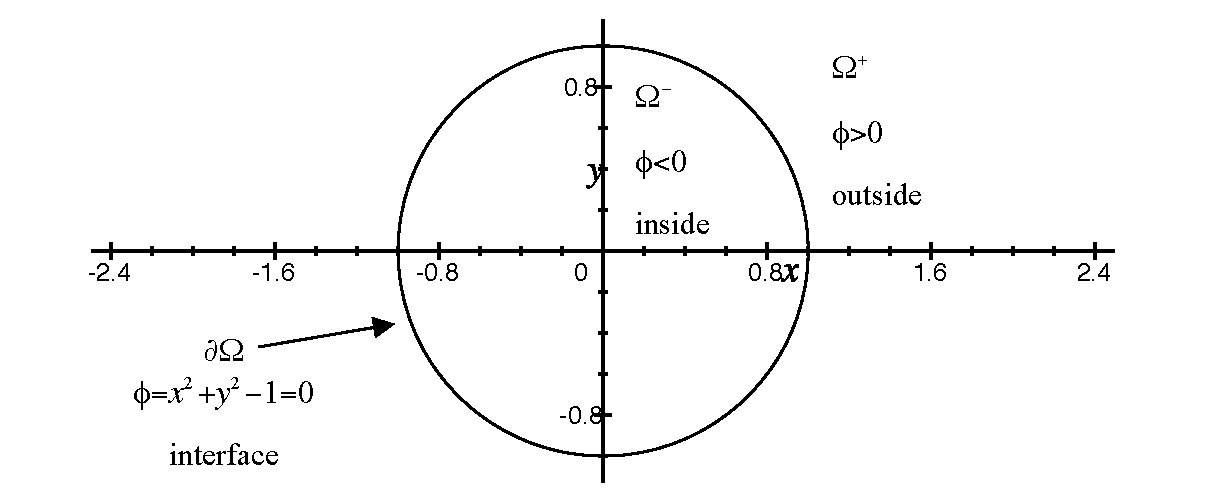
\includegraphics[width=\textwidth]{figures/df/implicit-function}
	\caption{隐式函数 $\phi(x, y) = x^{2} + y^{2} − 1$ 定义了区域 $\Omega^{−}$ 和 $\Omega^{+}$,同时也定义了这两个区域 的交界面$\partial\Omega$ ,即隐式表面}
	\label{f:df-implicit-function}
\end{figure}

隐式的交界面表述定义一个交界面为某个函数的等量线(ioscontour)\myindex{等量线}{ioscontour} ,例如,函数 $\phi(x,y=x^{2}+y^{2}-1) $的所有 0 等量线就是所有满足 $\phi(x,y) = 0$的点,这正好等于集合 $\partial\Omega = \{\vec{x}\mid |\vec{x}| = 1\}$,这可以从图\ref{f:df-implicit-function}中看出。这里隐式函 数 $\phi(x,y)$ 定义在二维的空间,而定义交界面的等量线却是一维的。更一般地, 在空间 $R^{n}$ 中,隐式函数 $\phi(\vec{x})$ 定义在所有 $\vec{x} \in R^{n}$ 上,而其等量线的维度为 $n − 1$。

所以,为了表述一个隐式表面,我们需要更多的空间存储这些点,因为隐 式函数 $\phi(\vec{x})$ 定义在 $R^{n}$ 空间内,而其交界面的维度其实只有 $n − 1$。不过在后 面可以看到,我们可以一些方法来节省一些存储空间。




\subsubsection{基本属性}
因为 $\phi(\vec{x})$ 定义在 $\vec{x} \in R^{n}$ 空间,所以我们很容易判断一个点 $\vec{x}$ 是否位于隐 式表面上,这里只需要判断 $\phi(\vec{x}) = 0$ 是否成立即可。不仅如此,对于闭合的表 面,我们还可以通过 $\phi$ 的符号来唯一区别一个点位于该隐式表面的哪一边,即:

\begin{equation}
	\phi(\vec{x})=\begin{cases}
		<0 & \text{~如果~} \vec{x}\in\Omega^{-}\\
		=0 & \text{~如果~} \vec{x}\in\partial\Omega\\
		>0 & \text{~如果~} \vec{x}\in\Omega^{+}
	\end{cases}
\end{equation}

这种属性也可以通过图\ref{f:df-implicit-function}看出来,我们将在后面介绍的距离函数也是满足这种条件的。

在显式表面表述中,这是很难去区分一个点是位于交界面的内部还是外部 的,因为其维度为 $n − 1$,其缺乏很多关于空间的信息。在这种情况下,一个比 较标准的流程是从要查询的点的位置 $P$ 向任意一个无穷远的位置发出一条光 线,然后数该光线与交界面相交的次数,如果相交次数为偶数,则该点位于交界面的外部,否则其相交次数为奇数,则该点位于交界面的内部,这种规则称为偶奇规则(even-odd rule)\myindex{偶奇规则}{even-odd rule},如图\ref{f:df-non-zero_winding}左下图所示。

\begin{figure}
	\sidecaption
	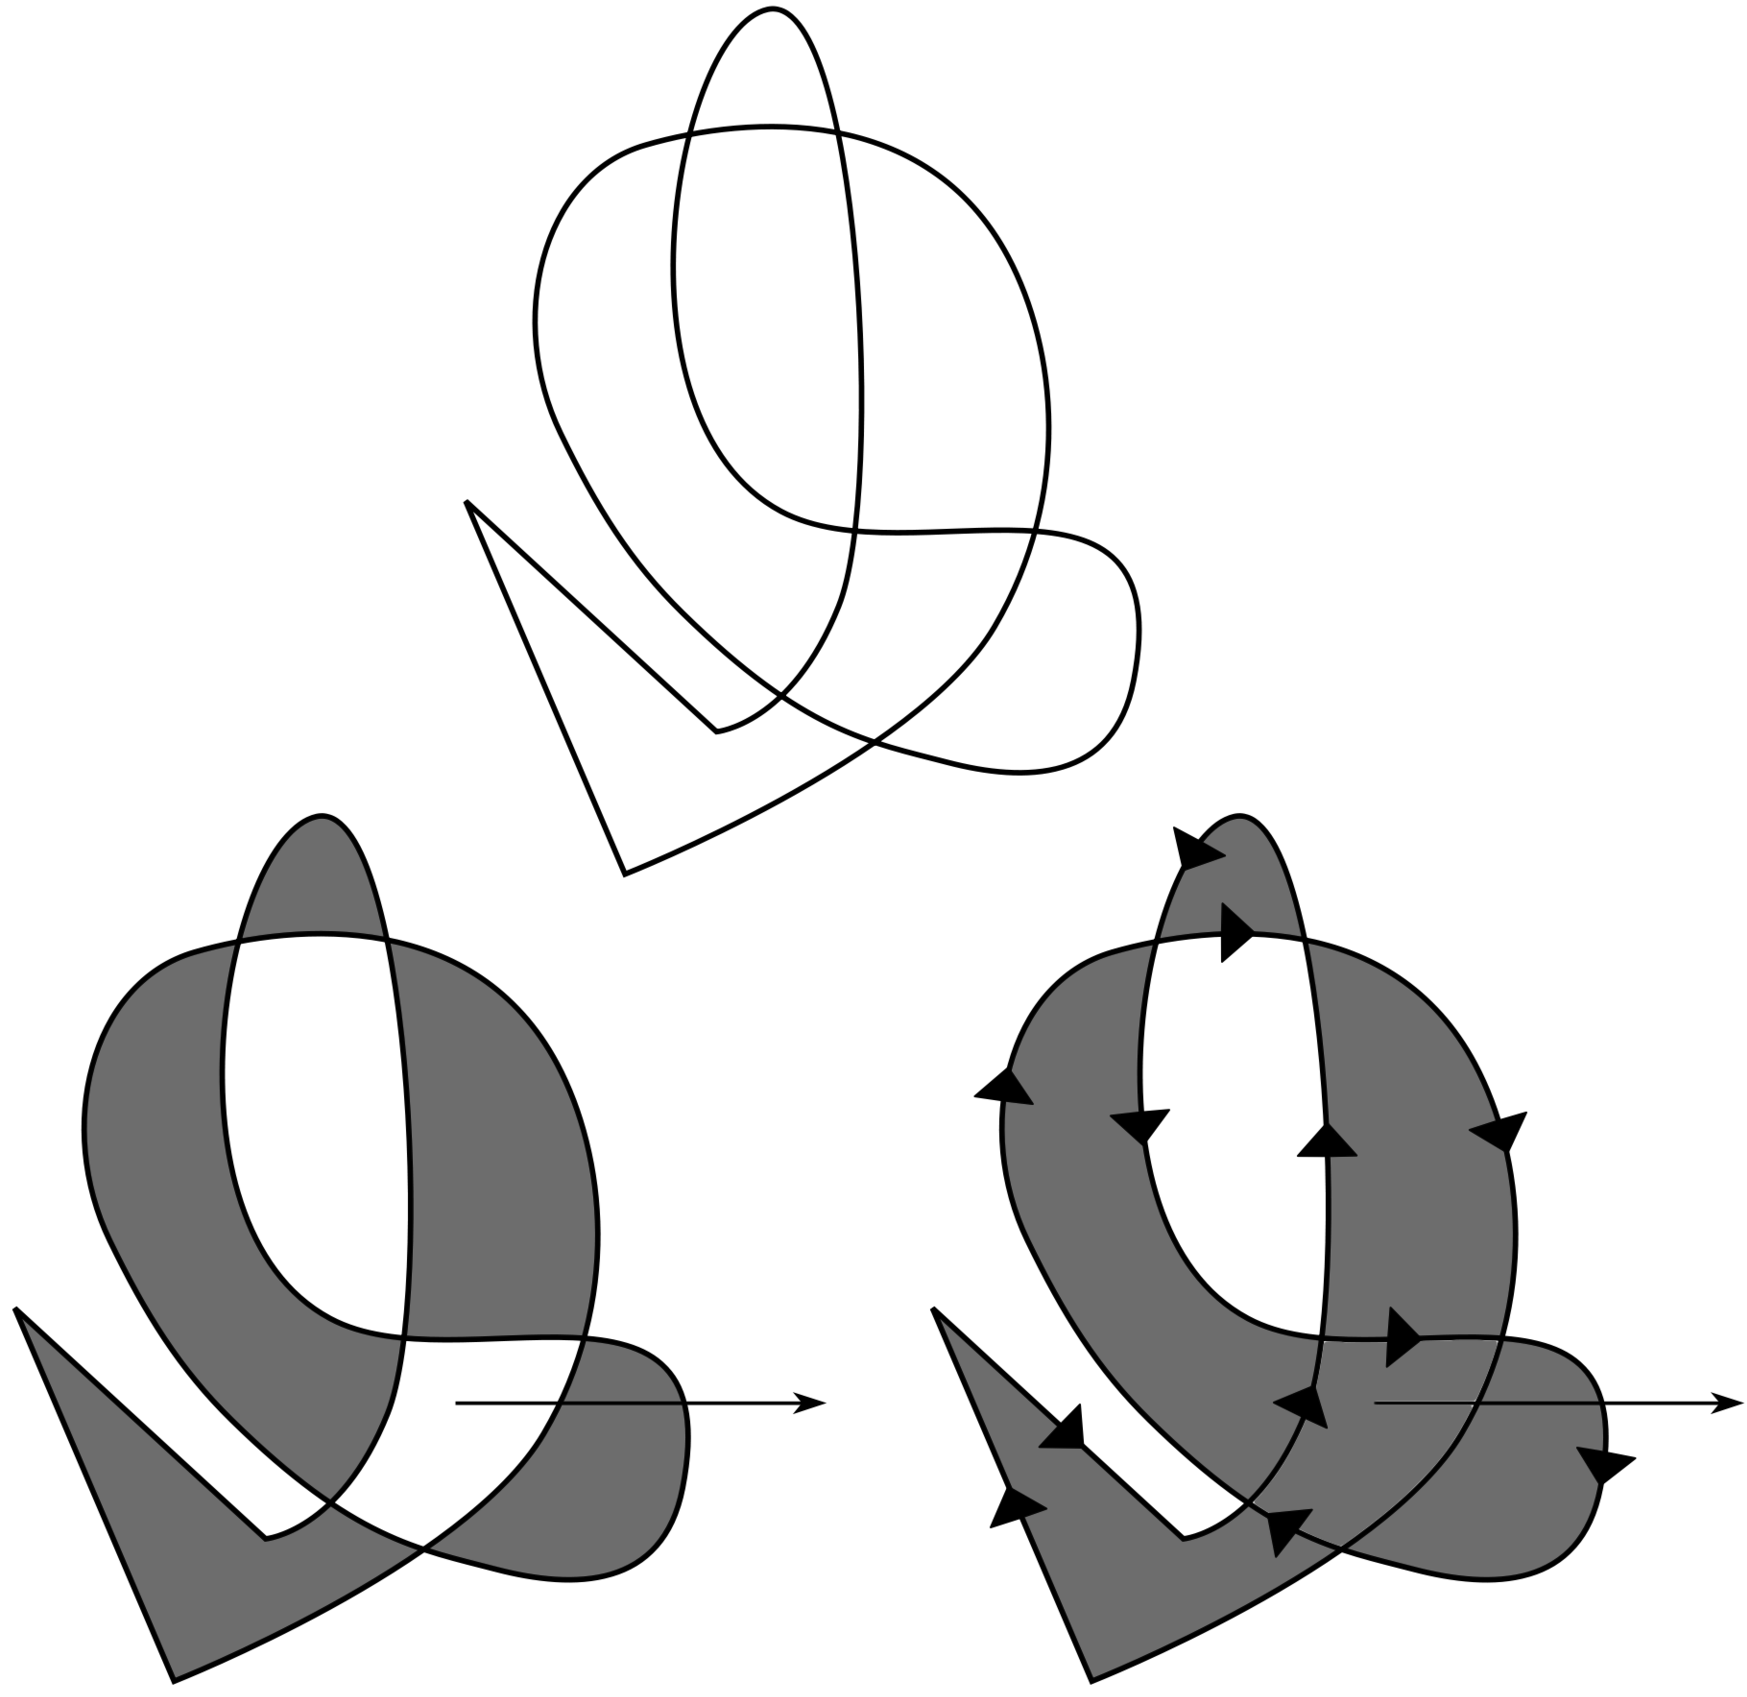
\includegraphics[width=0.5\textwidth]{figures/df/Even-odd_and_non-zero_winding_fill_rules}
	\caption{判定一个点是否位 于一个曲线 (上) 内部的两 种方法:即偶奇规则 (左下) 和非零数缠绕 (右下),这 两种方法都是从被测试的点 P 向任意一个无穷远的位 置发射一条光线,然后通过 相应的规则通过计数来判断 该点是否位于曲线内部(图 片来自 Wikipedia)}
	\label{f:df-non-zero_winding}
\end{figure}

另一种可用的方法称为非零数缠绕(non-zero winding rule)\myindex{非零数缠绕}{non-zero winding rule},与偶奇规则 不同的是,这种方法依赖于知道曲线上每一部分的绘制方向,它的计数规则如 下,对于每一个顺时针相交的计数为 +1,每个逆时针相交的计数为-1,所谓顺 时针相交是指相交的曲线从左向右穿过光线,反之则为逆时针相交。如果最后 总的计数为 0,则该点位于曲线的外部,否在位于内部,如图\ref{f:df-non-zero_winding}右下图所示。



\subsubsection{表面法线}
对于一个隐式表面 $\phi(\vec{x}) = 0$,其法线矢量 $\vec{N}$ 可以由其梯度给出,即:

\begin{equation}\label{e:df-normal}
	\vec{N}=\nabla\phi=\Biggl(\cfrac{\partial\phi}{\partial x},\cfrac{\partial\phi}{\partial y},\cfrac{\partial\phi}{\partial z}\Biggl)
\end{equation}

\cite{b:AnIntegratedIntroductiontoCG}提供了上述结论的一个证明,这个证明需要使用到链式法则(chain rule)\mathindex{链式法则}{chain rule}。假设 $P (t) = (x(t), y(t), z(t))$ 是表面 $\phi(\vec{x}) = 0$ 上的一个参 数化的曲面,则有:

\begin{equation}
	\phi(x(t),y(t),z(t))=0
\end{equation}

\noindent 使用链式规则有:

\begin{equation}
	\cfrac{\partial\phi}{\partial x}\cfrac{{\rm d}x}{{\rm d}t}+\cfrac{\partial\phi}{\partial y}\cfrac{{\rm d}y}{{\rm d}t}+\cfrac{\partial\phi}{\partial z}\cfrac{{\rm d}z}{{\rm d}t}=\cfrac{{\rm d}\phi}{{\rm d}t}=0
\end{equation}

\noindent 因此:

\begin{equation}
	\underbrace{\nabla\phi}_{\rm Gradient}\cdot\underbrace{P^{'}(t)}_{\rm Derivate}=\underbrace{\Biggl(\cfrac{\partial\phi}{\partial x},\cfrac{\partial\phi}{\partial y},\cfrac{\partial\phi}{\partial z}\Biggl)}_{\rm Normal vector}\cdot\underbrace{\Biggl(\cfrac{{\rm d}x}{{\rm d}t},\cfrac{{\rm d}y}{{\rm d}t},\cfrac{{\rm d}z}{{\rm d}t}\Biggl)}_{\rm Tangent vector}=0
\end{equation}

\noindent 所以:

\begin{equation}
	\vec{N}=\nabla\phi=\Biggl(	\cfrac{\partial\phi}{\partial x},\cfrac{\partial\phi}{\partial y},\cfrac{\partial\phi}{\partial z}\Biggl)
\end{equation}

因为交界面的隐式表述是嵌入在一个更高维度的作用域中,所以是这个更 高维度的作用域包含更多的信息是有用的。例如,与上面讨论的仅在交界面上 对每个位置定义一个单位法线矢量不同,我们可以使用式\ref{e:df-normal}在该作用域上每 个位置处定义一个法线函数 $\vec{N}$ ,这样就使得交界面上的法线嵌入在了这个法线 函数中,如图\ref{f:df-surface-normal}所示。

\begin{figure}
	\sidecaption
	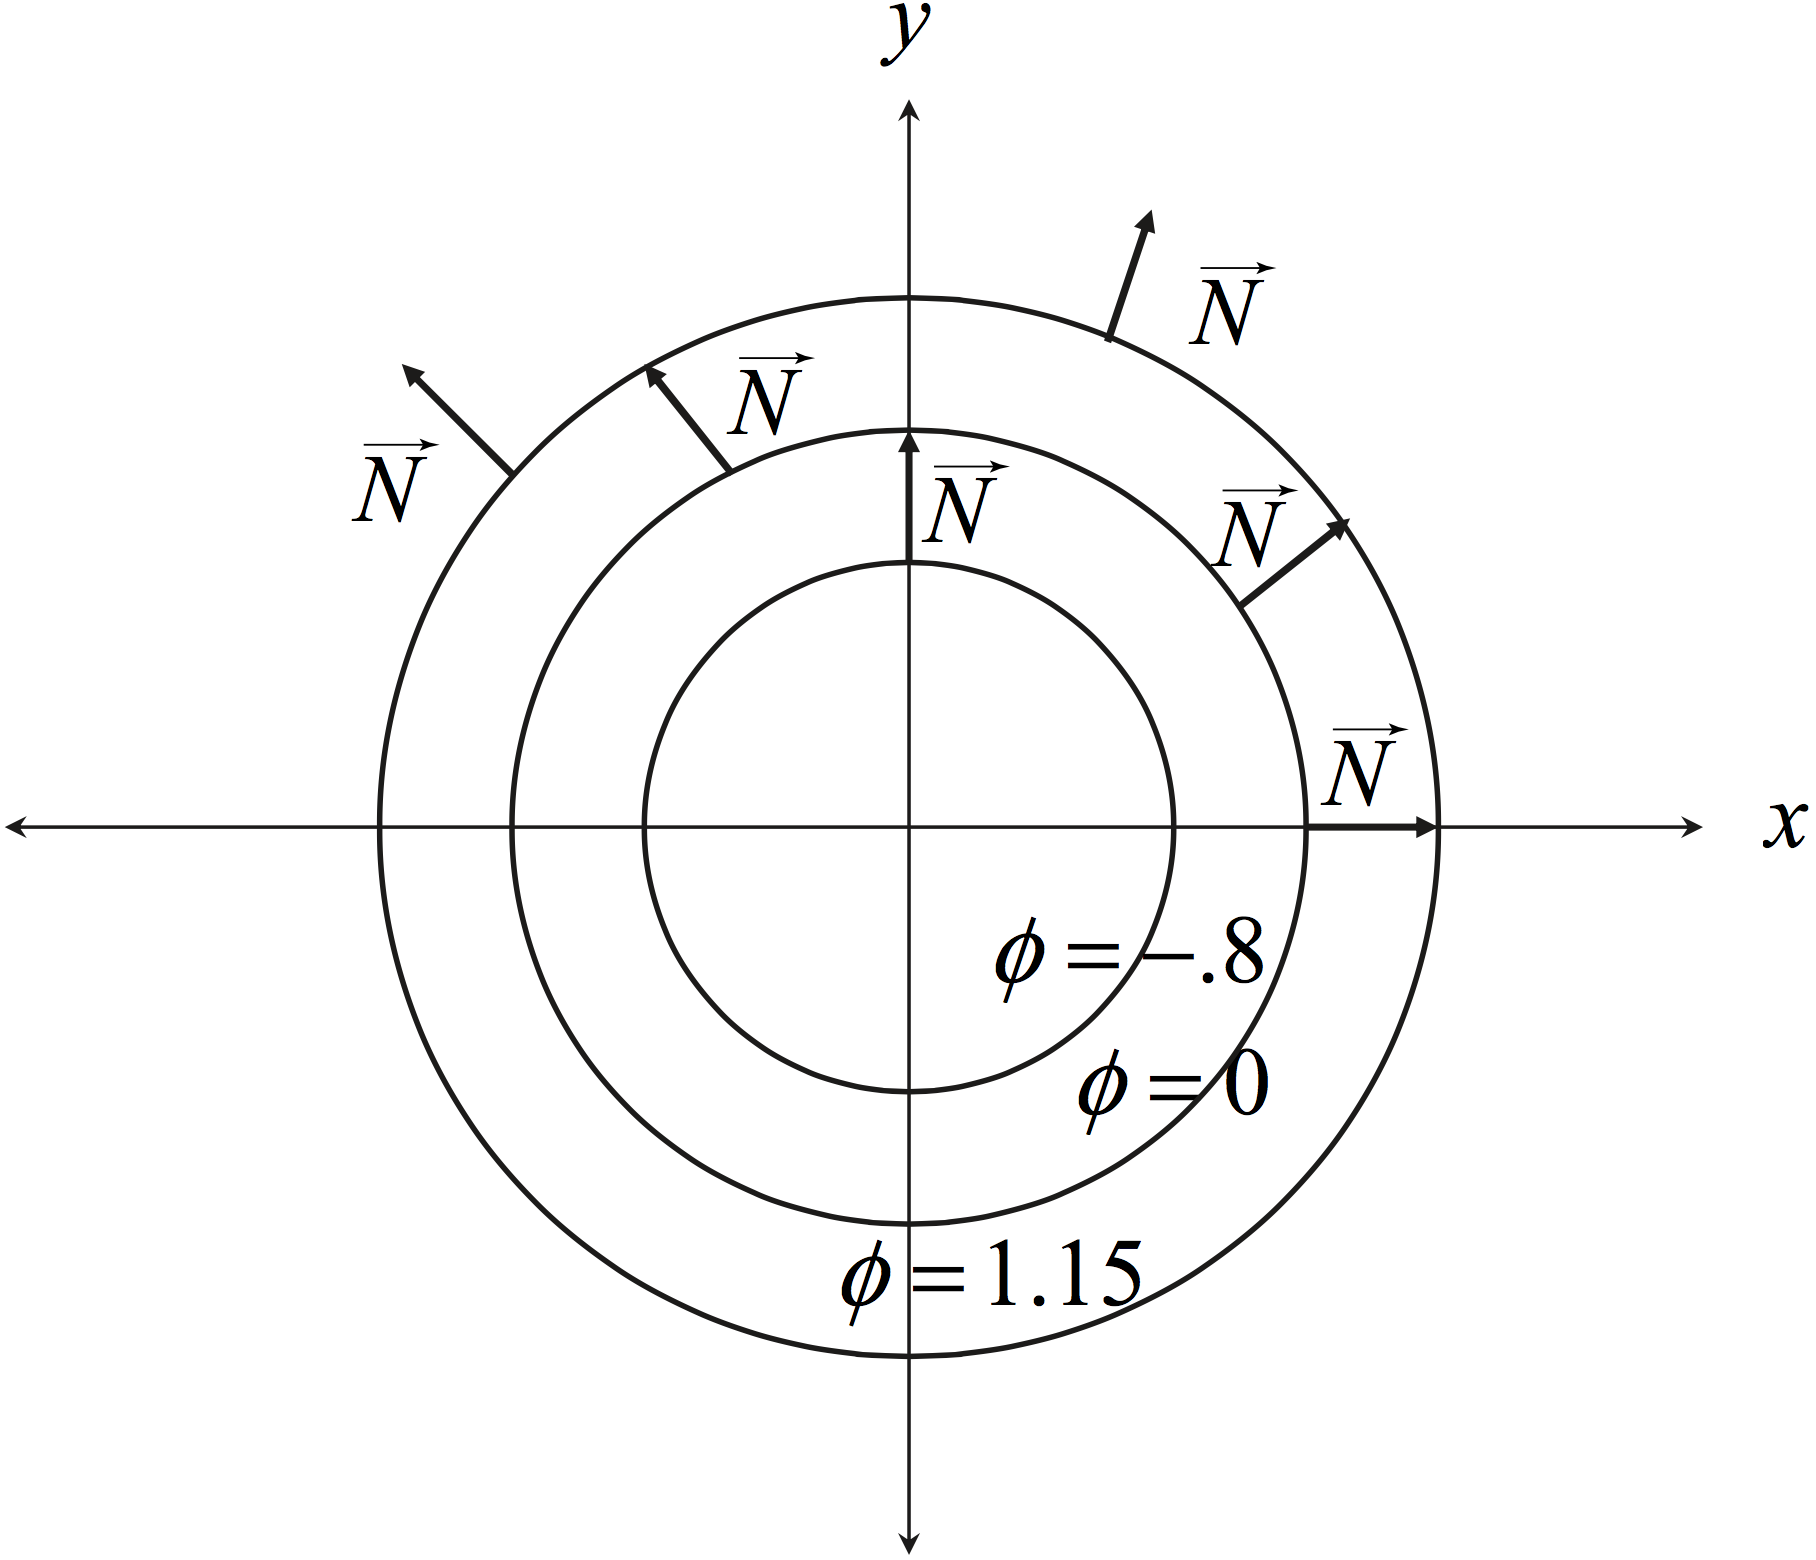
\includegraphics[width=0.45\textwidth]{figures/df/gradient-of-implicit-function}
	\caption{一个二维空间上隐式函数 $\phi(\vec{x}) = x^{2} + y^{2} − 1$ 的几个等量线,其中在全部 空间范围内,即包括交界面上,交界面内部及外部,这里列出了几个代表性的法线}
	\label{f:df-surface-normal}
\end{figure}



\subsubsection{布尔操作}
隐式函数使得布尔操作(boolean operations)\myindex{布尔操作}{boolean operations}变得非常简单,这使得一些更高级的构造实体几何(constructive solid geometry,CSG)\myindex{构造实体几何}{constructive solid geometry}操作也很容易地使用,如图\ref{f:df-csg-tree}所示。这是非常重要的,例如,在计算机辅助(computer-aided design,CAD)设计中,如果 $\phi_1$ 和 $\phi_2$ 是两个不同的隐式函数,则下述表述和操作是成立的:

\begin{itemize}
	\item $\phi(\vec{x}) = \min(\phi_1(\vec{x}), \phi_2(\vec{x}))$ 表示在区域 $\phi_1$ 和 $\phi_2$ 内部的联合;
	\item  $\phi(\vec{x}) = \max(\phi_1(\vec{x}), \phi_2(\vec{x}))$ 则表示区域 $\phi_1$ 和 $\phi_2$ 内部的相交;
	\item $\phi_1(\vec{x})$ 的补集可以定义为 $\phi(\vec{x}) = −\phi_1(\vec{x})$;
	\item $\phi(\vec{x}) = \max(\phi_1(\vec{x}), −\phi_2(\vec{x}))$ 表示从区域 $\phi_1$ 内部减去区域 $\phi_2$ 的内部。
\end{itemize}

\begin{figure}
	\sidecaption
	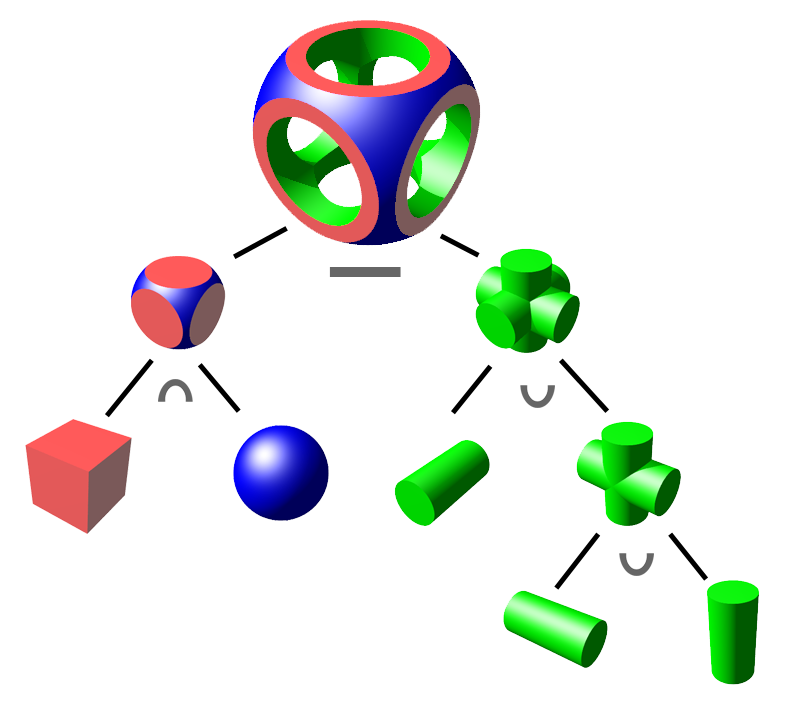
\includegraphics[width=0.5\textwidth]{figures/df/Csg-tree}
	\caption{CSG 物体可以表述为一个二进制树,其中的每个叶子表示一个基元,而每个节点表示一个操作,在图中,这些节点包含的操作包括相交,联合以及相减(图片来自 Wikipedia)}
	\label{f:df-csg-tree}
\end{figure}

在下一节,我们将以有符号的距离函数为例,说明隐式函数的布尔操作。



\subsection{有符号的距离函数}
在上一节,我们这样定义了一个隐式函数:它在内部区域 $\Omega^{−}$ 内的形式为 $\phi(\vec{x}) \leq 0$,在外部区域 $\Omega^{+}$ 的形式为 $\phi(\vec{x}) \geq 0$,而在交界面 $\partial\Omega$ 上的形式为 $\phi(\vec{x}) = 0$,但是一个隐式函数看起来到底是什么样的呢?这一节我们将讨论隐 式函数的其中一个特殊的子集:即有符号距离函数,它的函数值在内部区域是 一个正数,在外部区域是一个负数,在边界上的值则为 0。

对于全部 $\vec{x}_I \in\partial\Omega$,一个距离函数(distance function)\myindex{距离函数}{distance function}定义为:

\begin{equation}
	d(\vec{x})=\min (|\vec{x}-\vec{x}_I|)
\end{equation}

上式间接地说明,$d(\vec{x}) = 0$ 位于边界 $\vec{x}\in\partial\Omega$ 上。在几何上,函数 $d$ 可以通过这样的方式构建,如果 $\vec{x}\in \partial\Omega$,则 $d(\vec{x}) = 0$,否则,对于一个给定的点 $\vec{x}$,我 们找出边界 $\partial\Omega$ 上距离点 $\vec{x}$ 最近的点并标记该点为 $\vec{x}_C$ ,则有 $d(\vec{x}) = |\vec{x} − \vec{x}_C |$, 如图\ref{f:df-distance-function}所示。

\begin{figure}
	\sidecaption
	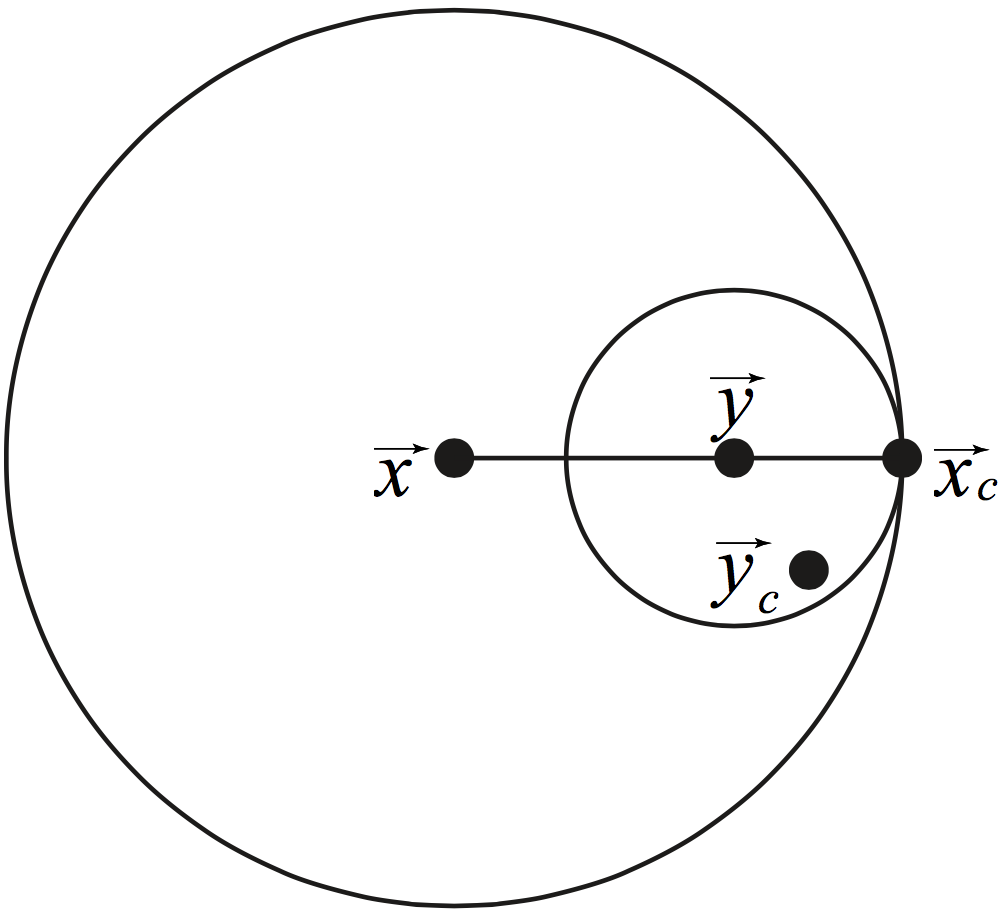
\includegraphics[width=0.4\textwidth]{figures/df/distance-function}
	\caption{边界上的点 $\vec{x}_C$ 是 距离点 $\vec{x}$ 和 $\vec{y}$ 最近的点, 所以这两个点的距离函数值 $d$ 就是这两个点各自到 $\vec{x}_C$ 的距离}
	\label{f:df-distance-function}
\end{figure}

对于所有 $\vec{x}$,一个有符号距离函数(signed distance function,SDF)\myindex{有符号距离函数}{signed distance function}是一个满足 $|\phi(\vec{x})| = d(\vec{x})$ 的隐式函数 $\phi$。因此:

\begin{equation}
	\phi(\vec{x})=\begin{cases}
		d(\vec{x})=0 & \vec{x}\in\partial\Omega \\
		-d(\vec{x}) & \vec{x}\in \Omega^{-} \\
		d(\vec{x}) & \vec{x}\in \Omega^{+}
	\end{cases}
\end{equation}

不难看出,有符号距离函数拥有上节讨论的隐式函数的所有属性。\cite{w:distance-function}提供了一些基本基元类型的距离函数,这里同时包含了一些简 单的代码可以直接用在例如着色器或者其它地方,如其中关于球面的有符号距离函数如表\ref{t:df-dist-function-1}所示。

\begin{table}
\begin{tabular}{m{3.0cm}m{7.cm}} 
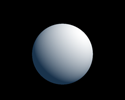
\includegraphics[width=0.21\textwidth]{figures/df/sphere} &
	 \begin{lstlisting}
Sphere - signed:
float sdSphere(vec3 p, float s)
{
  return length(p)-s;
}
\end{lstlisting} \\
   
\includegraphics[width=0.21\textwidth]{graphics/df/torus} & 
    \begin{lstlisting}
Torus - signed:
float sdTorus(vec3 p, vec2 t )
{
  vec2 q = vec2(length(p.xz)-t.x,p.y);
  return length(q)-t.y;
}
   \end{lstlisting}
\end{tabular}
\caption{关于球面和环形球面两个基元的简单有符号距离函数(图片和代码来自\cite{w:distance-function})}
\label{t:df-dist-function-1}
\end{table}

正如前面的内容所述,隐式函数之间的布尔操作是非常简单,\cite{w:distance-function}也提供了一些简单的函数用于组合距离函数,如表\ref{t:df-dist-function-2}所示。

\begin{table}
\begin{tabular}{m{3cm}m{7.cm}} 
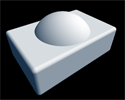
\includegraphics[width=0.21\textwidth]{graphics/df/union} &
	 \begin{lstlisting}
Union:
float opU(float d1, float d2)
{
    return min(d1,d2);
}
\end{lstlisting} \\
   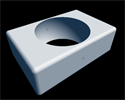
\includegraphics[width=0.21\textwidth]{graphics/df/substraction} & 
    \begin{lstlisting}
Substraction:
float opS(float d1, float d2)
{
    return max(-d1,d2);
}
   \end{lstlisting}
\end{tabular}
\caption{两个距离函数的组合示例:联合和相减,其中参数 d1 和 d2是两个待组合的距离函数的函数值(图片和代码来自 \cite{w:distance-function})}
\label{t:df-dist-function-2}
\end{table}

此外,\cite{w:distance-function}还提供了一些函数用于对距离函数执行形变操作,如图\ref{f:df-disform}所示,我们将在后面的章节中进一步讨论这些内容。

\begin{figure}
	\begin{subfigure}[b]{0.5\textwidth}
		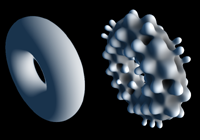
\includegraphics[width=\textwidth]{figures/df/displacement}
		\caption{移位}
	\end{subfigure}
	\begin{subfigure}[b]{0.5\textwidth}
		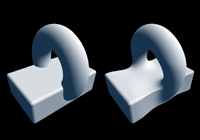
\includegraphics[width=\textwidth]{figures/df/blend}
		\caption{混合}
	\end{subfigure}
	\caption{一些距离函数形变的例子,这里的移位形变使用 $\sin(20 \times p.x)\times\sin(20\times p.y)\times\sin(20\times p.z)$ 作为一个移位模式 (图片和代码来自\cite{w:distance-function})}
	\label{f:df-disform}
\end{figure}

给定一个有符号距离函数,我们可以得到定义域中任意一个点到离该点最 近的表面的距离,这可以用在光线步进或球体追踪当中,我们将在第\ref{sec:df-rendering-of-implicit}节讨论这些内容。此外,通过 \cite{w:distance-function} 提供的函数,我们还可以从一个基元的显式 表述中计算出一个距离函数。

但是现实世界中的物体要比这些简单的基元复杂得多,例如一个物体可能 由成千上万个三角形组成,这可能非常复杂。我们可以对距离场进行预计算并 存储在体积纹理中,也可以在 GPU 中实时计算,或者从一些分形中直接计算, 我们将在下一节更深入地讨论这些内容。



\section{场景的隐式表述}
本节将讨论关于隐式表面的表述,特别地,这里仅讨论距离场这种表述形 式。首先,我们会介绍几种常用的计算距离场的方法,然后,介绍距离场数据 怎样被存储于 GPU 当中,最后,我们会介绍一些在 GPU 中实时动态计算距 离场的方法。


\subsection{计算距离场}
距离函数表述了整个定义域内所有点到最近物体表面的距离,在实际运用 中我们通常只存储一些离散的位置,例如 3D 空间中一个规则的网格 $v$,或者 其它体积结构。传统的使用蛮力的方式计算网格 $v$ 内的点到一些物体表面最近 距离的方法非常简单:对于网格 $v$ 内的每一个体素,它到所有物体的距离都被 计算一次,这通过从该点向所有方向发射光线并存储最近的表面,最后只有数值最小的距离被存储,例如 Unreal Engine 4 就是使用这种方法生成离线的距离场,如图\ref{f:df-brute-force-method}所示。

\begin{figure}
	\sidecaption
	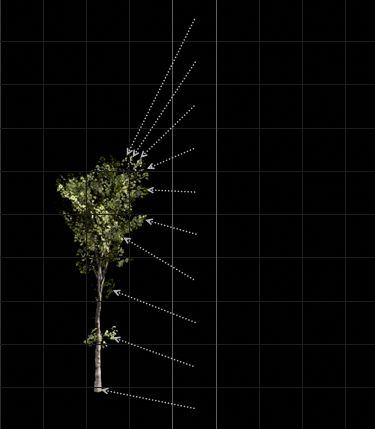
\includegraphics[width=0.5\textwidth]{figures/df/brute-force-method}
	\caption{在 Unreal Engine 4 中,网格的距离场使用蛮 力的方式生成,即对每个要计算的位置向所有方向发射光线,最后选取其中表面最近的那条光线的距离值(图片来自 Unreal Engine 4 官方文档)}
	\label{f:df-brute-force-method}
\end{figure}

尽管这种方法非常简单,它却非常耗时。另外一些比较具有实用性的方法 可以分成两大类:

\begin{enumerate}
	\item 第一类方法尝试放弃对那些距离较远的物体的光线追踪;
	\item 第二类方法仅在初始阶段计算一些特定区域内的距离,例如通常仅计算物 体内部或者物体表面很薄的一层空间范围,然后将这些计算出来的少量距离传播至整个场景,这种方法称为距离变换。
\end{enumerate}

这些方法虽然拥有较快的计算速度,然而其结果的精度却很低。在实践中, 例如在 Unreal Engine 4 中,蛮力方法用于在离线阶段预计算那些静态物体的 距离场,而这些加速的方法则可以用于实时阶段动态地计算少数动态物体的距 离场,当然 Unreal Engine 4 在实时阶段可能是用了一些其它加速方法。



\subsection{一般表面表述的距离场}
三角形网格可能是 3D 几何体最常使用的表面表述形式,因此怎样将这种 特定的三角形网格转化为有符号的距离场,变得尤其重要。通常我们仅能从一 种特定类型的三角形网格生成距离场,即那些闭合,有向的二维流形。

一个点到一个三角形的距离可以很简单地使用分析的方法得出,当一个点 $p$ 被投影到包含某个三角形的平面上时,其投影点 $p^{'}$ 会落于图\ref{f:df-calculating-distance-to-triangle}显式的7个区域之一,这7个区域可以分为三类情形\cite{a:3d-distance-fields-a-survey}:

\begin{figure}
	\sidecaption
	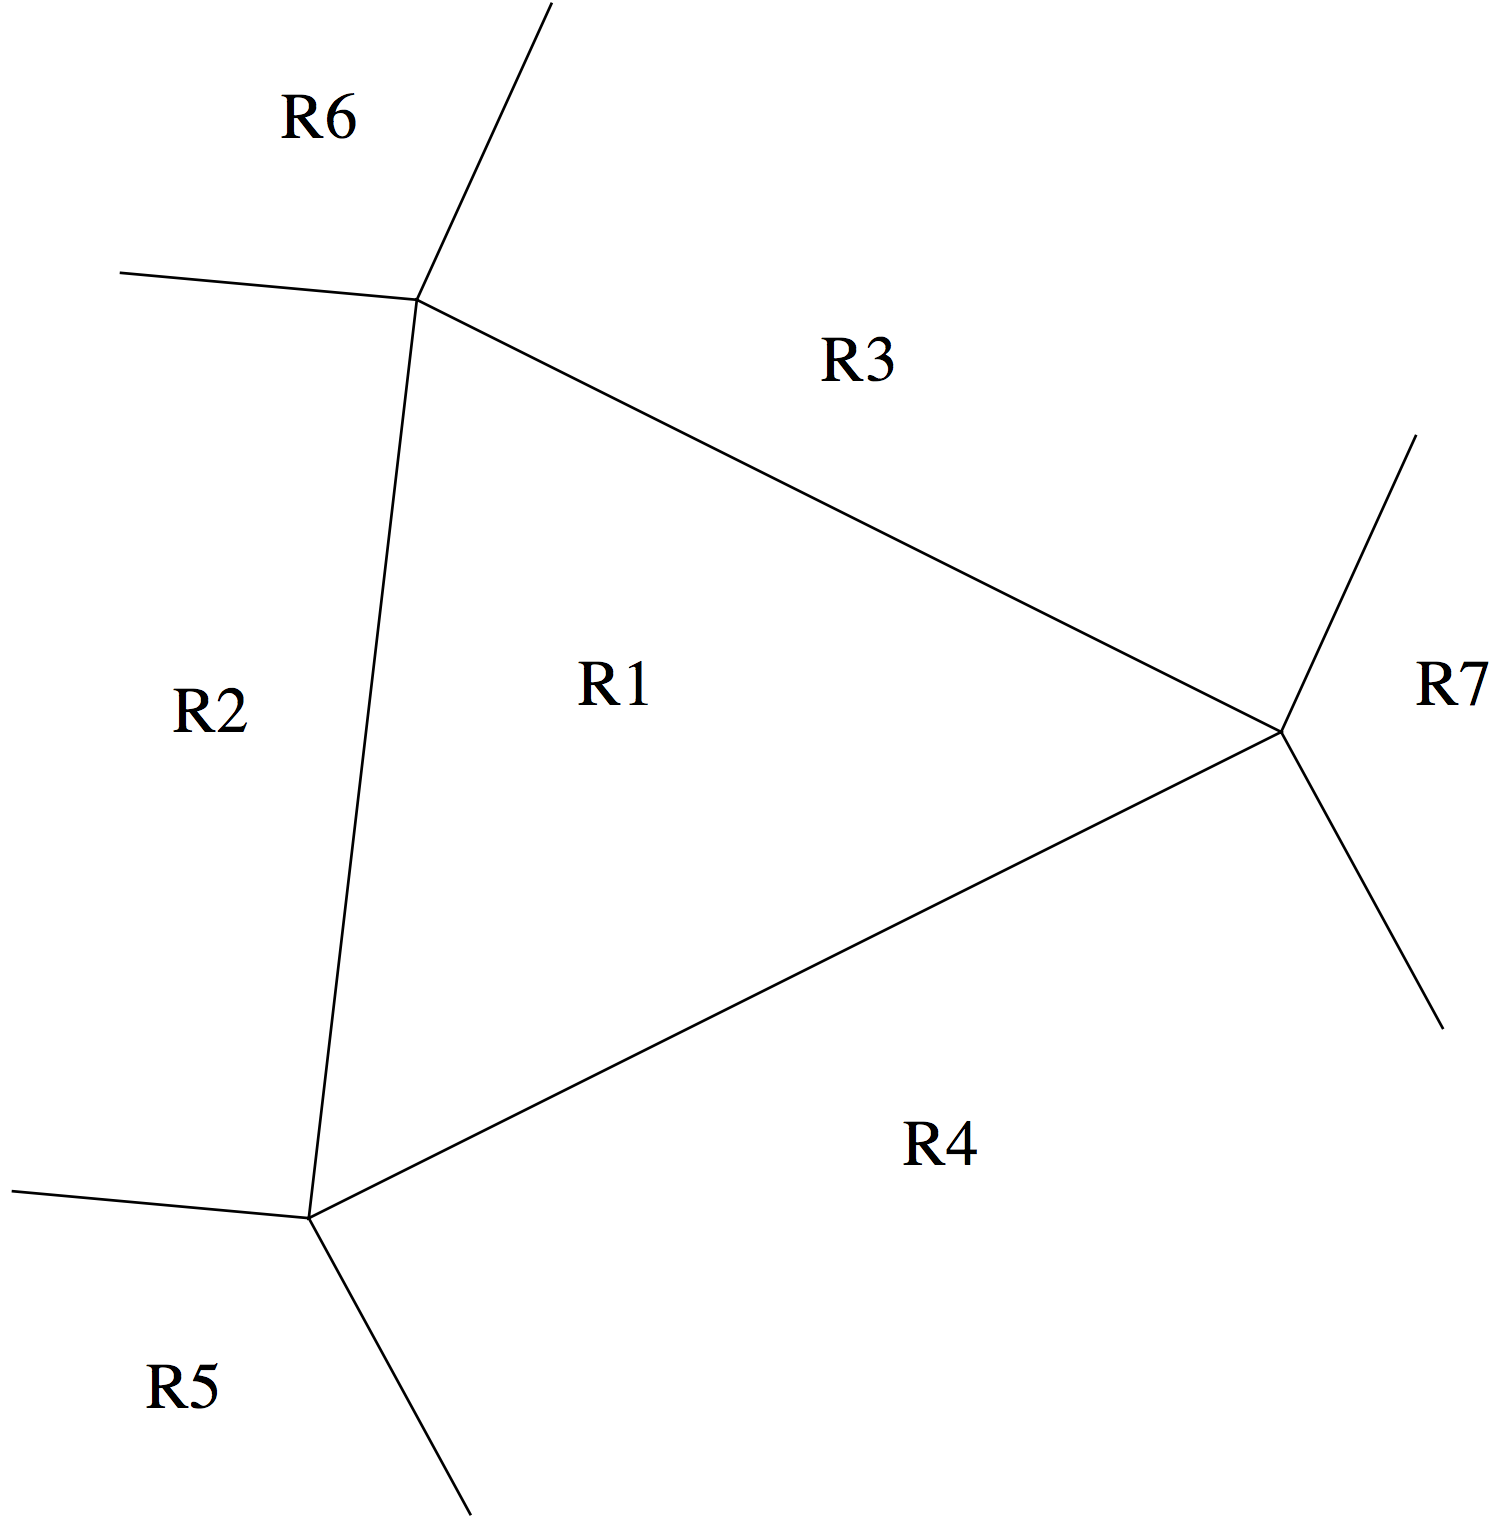
\includegraphics[width=0.45\textwidth]{figures/df/calculating-distance-to-triangle}
	\caption{计算一个点到一个三角形的距离:如果 $p$ 投影到区域 R1,则其距离为该点到三角形所在平面的距离,如果投影到区域 R2 − R4,则距离为该点到对应边的距离,如果投影到区域 R5 − R7,则其距离为点到对应顶点的距离}
	\label{f:df-calculating-distance-to-triangle}
\end{figure}

\begin{itemize}
	\item 如果点 $p^{'}$ 落于区域 R1,则点 p 到该三角形的距离就等于该点到包含这个三角形的平面的距离;
	\item 如果点 $p^{'}$ 落于区域R2,R3或R4,则点$p$到该三角形的距离等于该点到对 应边所在的直线的距离;
	\item 最后,如果点$p^{'}$落于区域 R5, R6 或 R7,则点 $p$ 到该三角形的距离等于该 点到对应顶点的距离。
\end{itemize}

这种蛮力的方法需要计算 $N \cdot M$ 次,其中 $N$ 为体素的数量,$M$ 为三角 形的数量,因此通常我们使用一些阶层式的结构使其对三角形的访问复杂度为 $O(\log M )$。

有时候,我们仅需要计算离表面一定距离内的距离值,这可以通过使用 三角形的包围盒来保证,只有那些近于某些距离的体素的距离值被计算,如 图\ref{f:df-close-triangle}所示,这种方法例如被使用在\cite{a:Incremental-Triangle-Voxelization}中。

\begin{figure}
	\sidecaption
	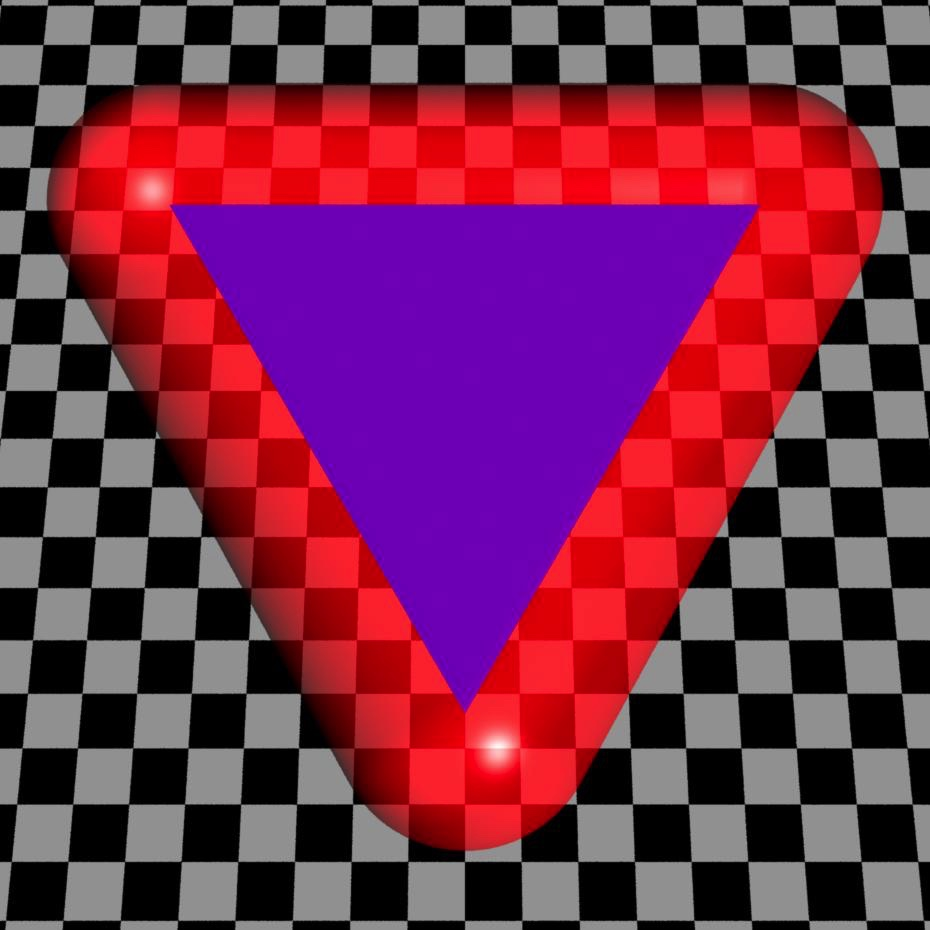
\includegraphics[width=0.35\textwidth]{figures/df/close-triangle}
	\caption{影响计算体素距离的三角形的3D区域}
	\label{f:df-close-triangle}
\end{figure}

当计算出距离的数值之后,我们还需要决定这个距离值的符号,这里最明 显的计算距离值的符号的方法是使用表面的法线。如果我们拥有一个满足 $C^{1}$ 的平滑曲面,则距离值的符号可以通过计算法线 $n$ 与一个方向矢量 $d$ 的点积求得,该方向矢量 $d$ 由得到的表面上最近的点执行我们希望计算的体素的位置,实际上,$d$ 的方向只可能指向法线 $n$ 的相同方向(如果被检测的点位于物体外部)或相反方向(如果被检测的点位于物体外部)。

然而三角形网格并不是满足 $C^{1}$ 的,因为三角形的边和顶点上并没有法线 的定义,所以\cite{a:3d-distance-fields-a-survey}对三角形的顶点和边定义了一个使用角度加权法线(angle weighted normal)\myindex{角度加权法线}{angle weighted normal}作为一个伪法线。为了计算顶点的角度加权法线,这里将所有该顶点相邻面的法线累加起来,其中每个法线被使用一个角度 加权,该角度等于该面的相交于该顶点的两条边形成的夹角,如图\ref{f:df-Computing-vertex-normals}所示。

\begin{figure}
	\sidecaption
	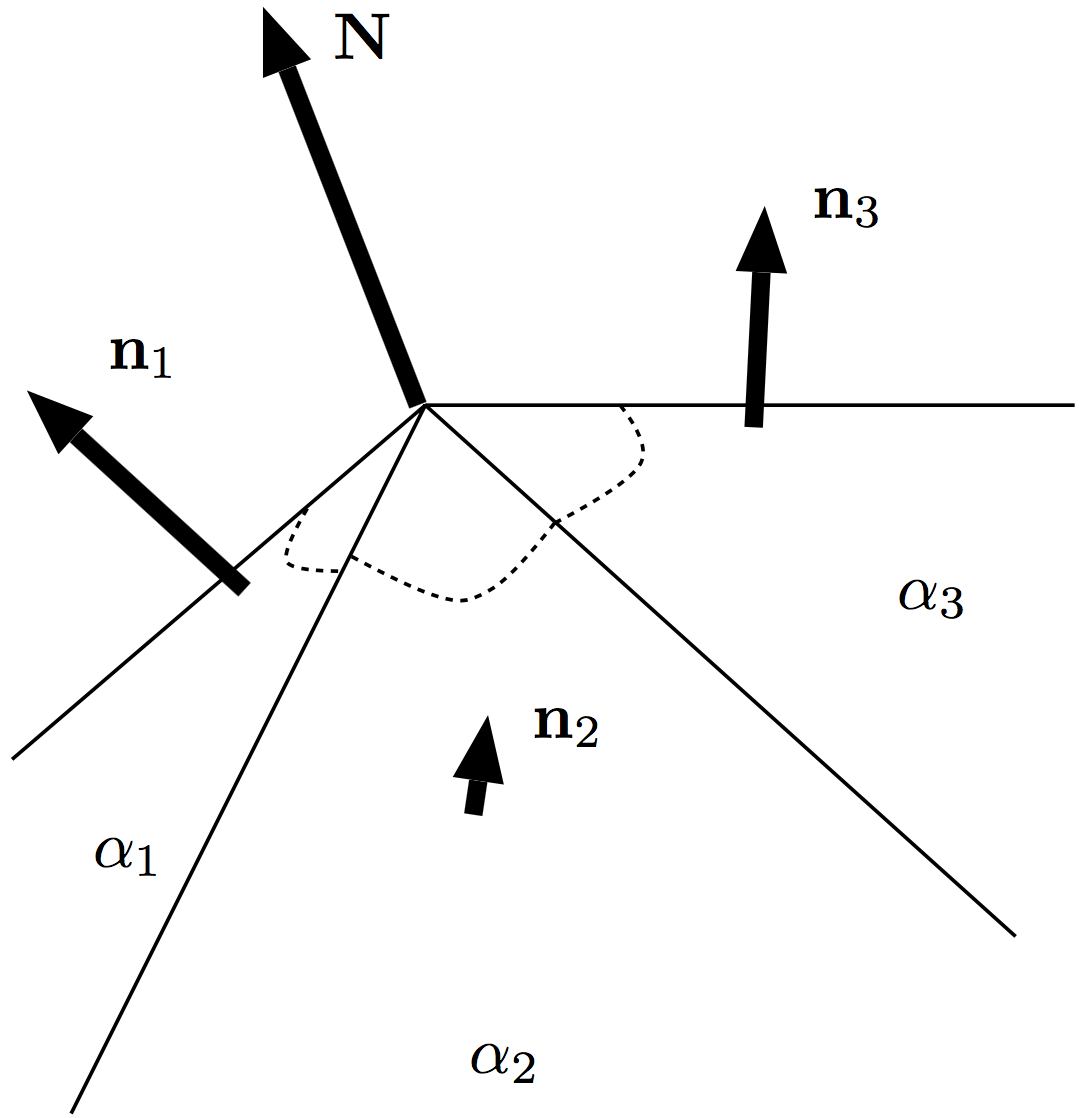
\includegraphics[width=0.4\textwidth]{figures/df/Computing-vertex-normals}
	\caption{角度加权法线示意图:$N=\cfrac{\sum_in_i a_i}{||\sum_in_ia_i||}$}
	\label{f:df-Computing-vertex-normals}
\end{figure}

对于一个任意未闭合网格的距离符号计算是非常麻烦的,在 Unreal Engine 4 中使用了一个简单的启发式用于决定一个点是否处于物体“内部”:当使用光线 追踪找到最近的表面之后,如果击中物体背面的光线的数量大于总共使用光线 数量的 50\%,则这个位置可以认为是位于物体“内部”的,如图\ref{f:df-ue4-sign}所示。

\begin{figure}
	\begin{subfigure}[b]{0.5\textwidth}
		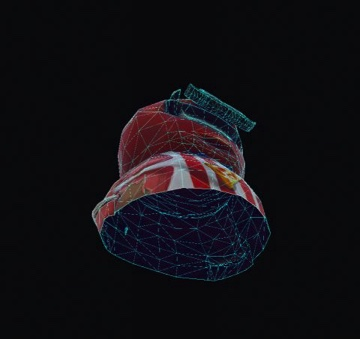
\includegraphics[width=\textwidth]{figures/df/ue4-sign-1}
		\caption{移位}
	\end{subfigure}
	\begin{subfigure}[b]{0.5\textwidth}
		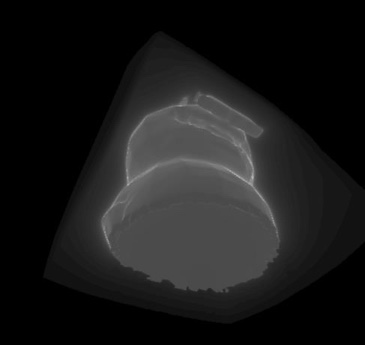
\includegraphics[width=\textwidth]{figures/df/ue4-sign-2}
		\caption{混合}
	\end{subfigure}
	\caption{Unreal Engine 4 使用了一个简单的启发式方法用于计算未闭合表面物体的距离场的符号(图片来自\cite{a:Dynamicocclusionwithsigneddistancefields})}
	\label{f:df-ue4-sign}
\end{figure}




\subsection{距离变换}
距离变换(distance transform,DT)\myindex{距离变换}{distance transform}后的原则是,我们可以根据表面的边 界生成一个靠近这个边界的边界条件,对于在这个边界条件内的体素,它们的 距离场可以使用上面介绍的任意直接方法(例如蛮力方法或者一些近似方法), 而剩下的区域则可以直接通过这些计算出的距离值推导出来,而不需要执行直 接的距离计算。

所以距离变换方法涉及两个阶段,第一个阶段是使用传统的直接方法计算 边界条件内部的体素的距离值,在第二阶段,则直接使用某种距离变换算法将 这些边界条件内的距离值传播到剩下的体积区域。由于边界区域外的距离值不 是直接计算出来的,因此这引入了一定的误差。距离变换算法可以分为两大类, 即切角距离变换和矢量距离变换。

切角距离变换(chamfer distance transform)\myindex{切角距离变换}{chamfer distance transform}通过查询一个关于相邻体素 位置的表来计算这些相邻体素的距离值,这个表称为一个距离模板(distance template)\myindex{距离模板}{distance template},最后加上这些距离模板中的值来作为这些相邻体素的距离值。

如表\ref{t:distance-template}所示,当处理一个新的体素时,首先将当前体素置于表格中心,其距离模板中的值为 0,以其左边的相邻体素为例,其模板值 $a = 1$,所以我们将 当前体素的距离值加上$a$作为该相邻体素的距离值。这里根据相邻关系(例如水平或者对角线),其添加的系数是不一样的,具体值可参见表\ref{t:distance-template}所示。此外 需要注意的是,距离模板中像个相邻体素的距离表示一个像素的距离,如果要使用大于或小于一个像素的分辨率,则每个模板值在被添加的时候需要乘以体素之间实际的距离,即这些模板值是体素之间真实距离的缩放系数。

\begin{table}
\begin{center}
	\begin{tabular}{|c|c|c|c|c|}
		\hline
		~2b~ & ~~c~~ & ~2a~ & ~~c~~ & ~2b~\\
		\hline
		c&b&a&b&c\\
		\hline
		2a&a&0&a&2a\\
		\hline
		c&b&a&b&c\\
		\hline
		2b&c&2a&c&2b\\
		\hline
	\end{tabular}
\end{center}
\caption{切角距离变换方法使用的距离模板,这里 $a=1,b=\sqrt{2},c=\sqrt{3}$}
\label{t:distance-template}
\end{table}

切角距离变换的精确度随着距离的增加而下降,使用一个更大分辨率的距 离模板可以提供更好的结果,一些切角距离变换的结果如图\ref{f:df-multi-distance-transform}所示,这里CDA是切角距离变换算法(chamfer distance transform algorithm)\myindex{切角距离变换算法}{chamfer distance transform algorithm}的缩写,我们可以看到对距离模板使用不同分辨率下变换结果的差异。

\begin{figure}
\begin{fullwidth}
	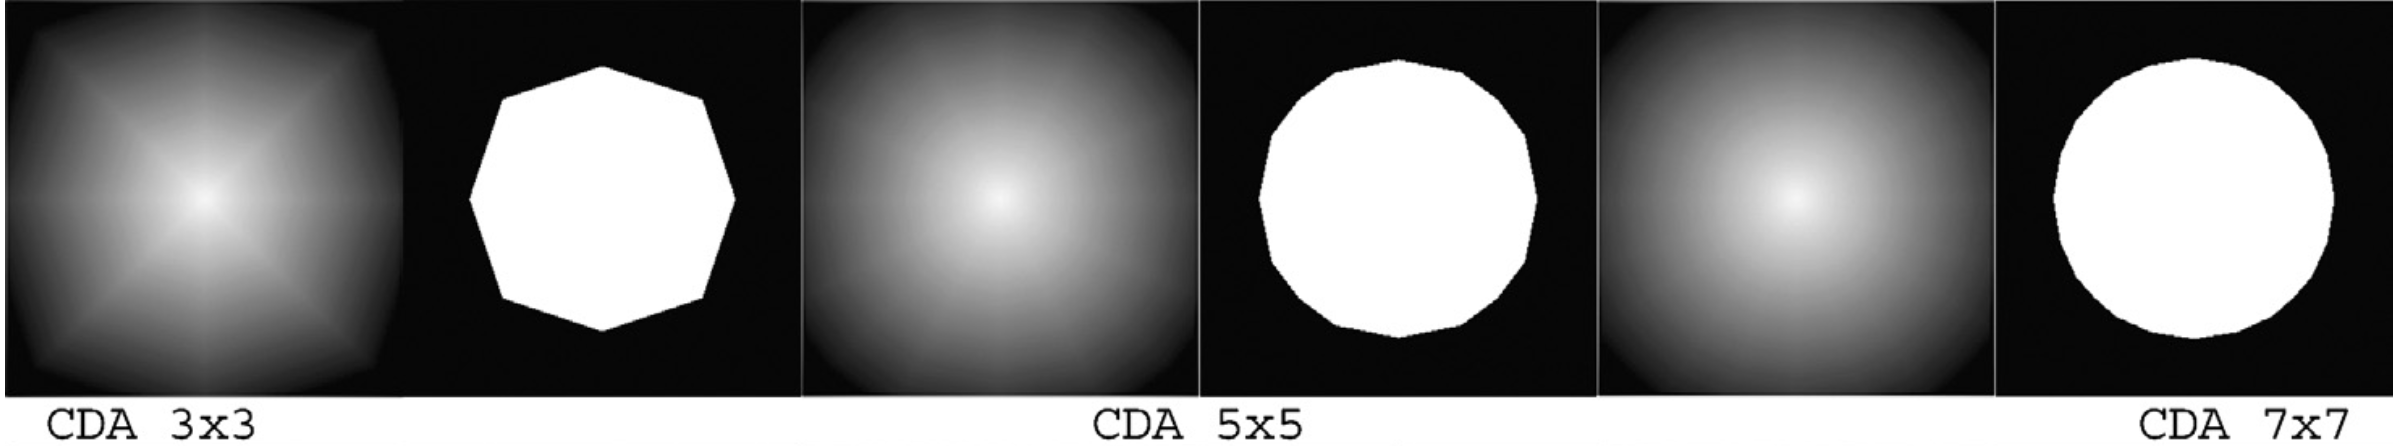
\includegraphics[width=\thewidth]{figures/df/multi-distance-transform}
	\caption{不同分辨率的切角距离变换算法作用于一个相同的输入图片的结果,其中输入图片的中心包含一个点,其理想的距离场应该是圆形的}
	\label{f:df-multi-distance-transform}
\end{fullwidth}
\end{figure}

\cite{a:dead-reckoning}基于切角距离变换算法作出修改,使其能够在不增加窗体 尺寸的情况下产生更精确的结果,请读者自行参考。

与切角距离变换算法的距离模板中直接存储一个标量值不同,矢量距离变换算法(vector distance transform)\myindex{矢量距离变换算法}{vector distance transform}对已处理的体素存储一个矢量,这个矢量由该体素的位置指向距离其最近表面位置,对于未处理的体素,其矢量值可以 通过查询一个矢量模板(vector template)\myindex{矢量模板}{vector template}计算出来。

所有的切角距离变换都是某种近似程度的矢量距离变换,矢量距离变换可 以提供更精确的结果,\cite{a:Euclidean-Distance-Mapping}和\cite{a:Vector-City-VDT}提供了更 详细的介绍,距离变换算法被大量使用在图像处理领域。



\subsection{距离场的表述}
一个 3D 的距离场可以存储在 GPU 的一个体积纹理中,但是那样将会消耗很大的内存,而在一个游戏场景中,整个游戏世界可能是无限的,并且在天空或者室内存在大量空白空间。因此我们希望寻找一些更好的表述方法,使之能够降低存储需求同时保持较好的精度。

本节将主要介绍两组表述方法,即适应性距离场和完全距离场,这些方法已经被广泛使用。虽然这些方法还衍生出了很多变种,我们这里仅讨论它们背 后的基本思路。



\subsubsection{适应性距离场}
因为规则采样的距离场有上面讨论的缺点,所以许多方法尝试使用一个阶 层式的网格,使其中那些空白区域可以被忽略掉。另一方面,一些细节表面需 要被更密集的采样,有些重要的区域也需要被更精确地表述。

适应性距离场(adaptive distance fields, ADF)\myindex{适应性距离场}{adaptive distance fields}使用一种适应性地,细节驱 动的采样方法,即对那些距离场包含更多细节的区域使用更高的采样密度,而 对那些更平滑的区域使用更低的采样密度。因此,适应性距离场可以达到任意 的精度要求,同时又只占用更少的内存。

为了更高效地处理按适应性的方式采样的数据,我们通常使用一个八叉树 结构来存储这些距离场数据。图\ref{f:df-adf}演示了在2D 空间(因此这里是四叉树结构)中的存储结构,在基于四叉树的适应性距离场表述中,每个四叉树的单元(cell)存储着其四个角的距离值,以及到父级和子级单元的指针。注意,这里和传统的四叉树是有区别的,传统的四叉树通常是处理单元中心的位置,而这里是考虑边角,例如我们可以将一个单元的一条边直接与表面重合,这样处理起来更方便,如果考虑单元中心,那在物体表面上单元就可能嵌入仅表面内部; 另外,在距离场中的每个体素单元内,我们需要能够计算所有位置的距离值,这可以通过对四个角的值插值计算出来,而如果每个单元仅存储单个值,则需要 借助相邻单元才能实现插值计算,然而在适应性距离场中,同一分辨率下相邻的单元可能并不存在,因为它们可能处于不同分辨上。

\begin{figure}
\begin{fullwidth}
	\begin{subfigure}[b]{0.5\thewidth}
		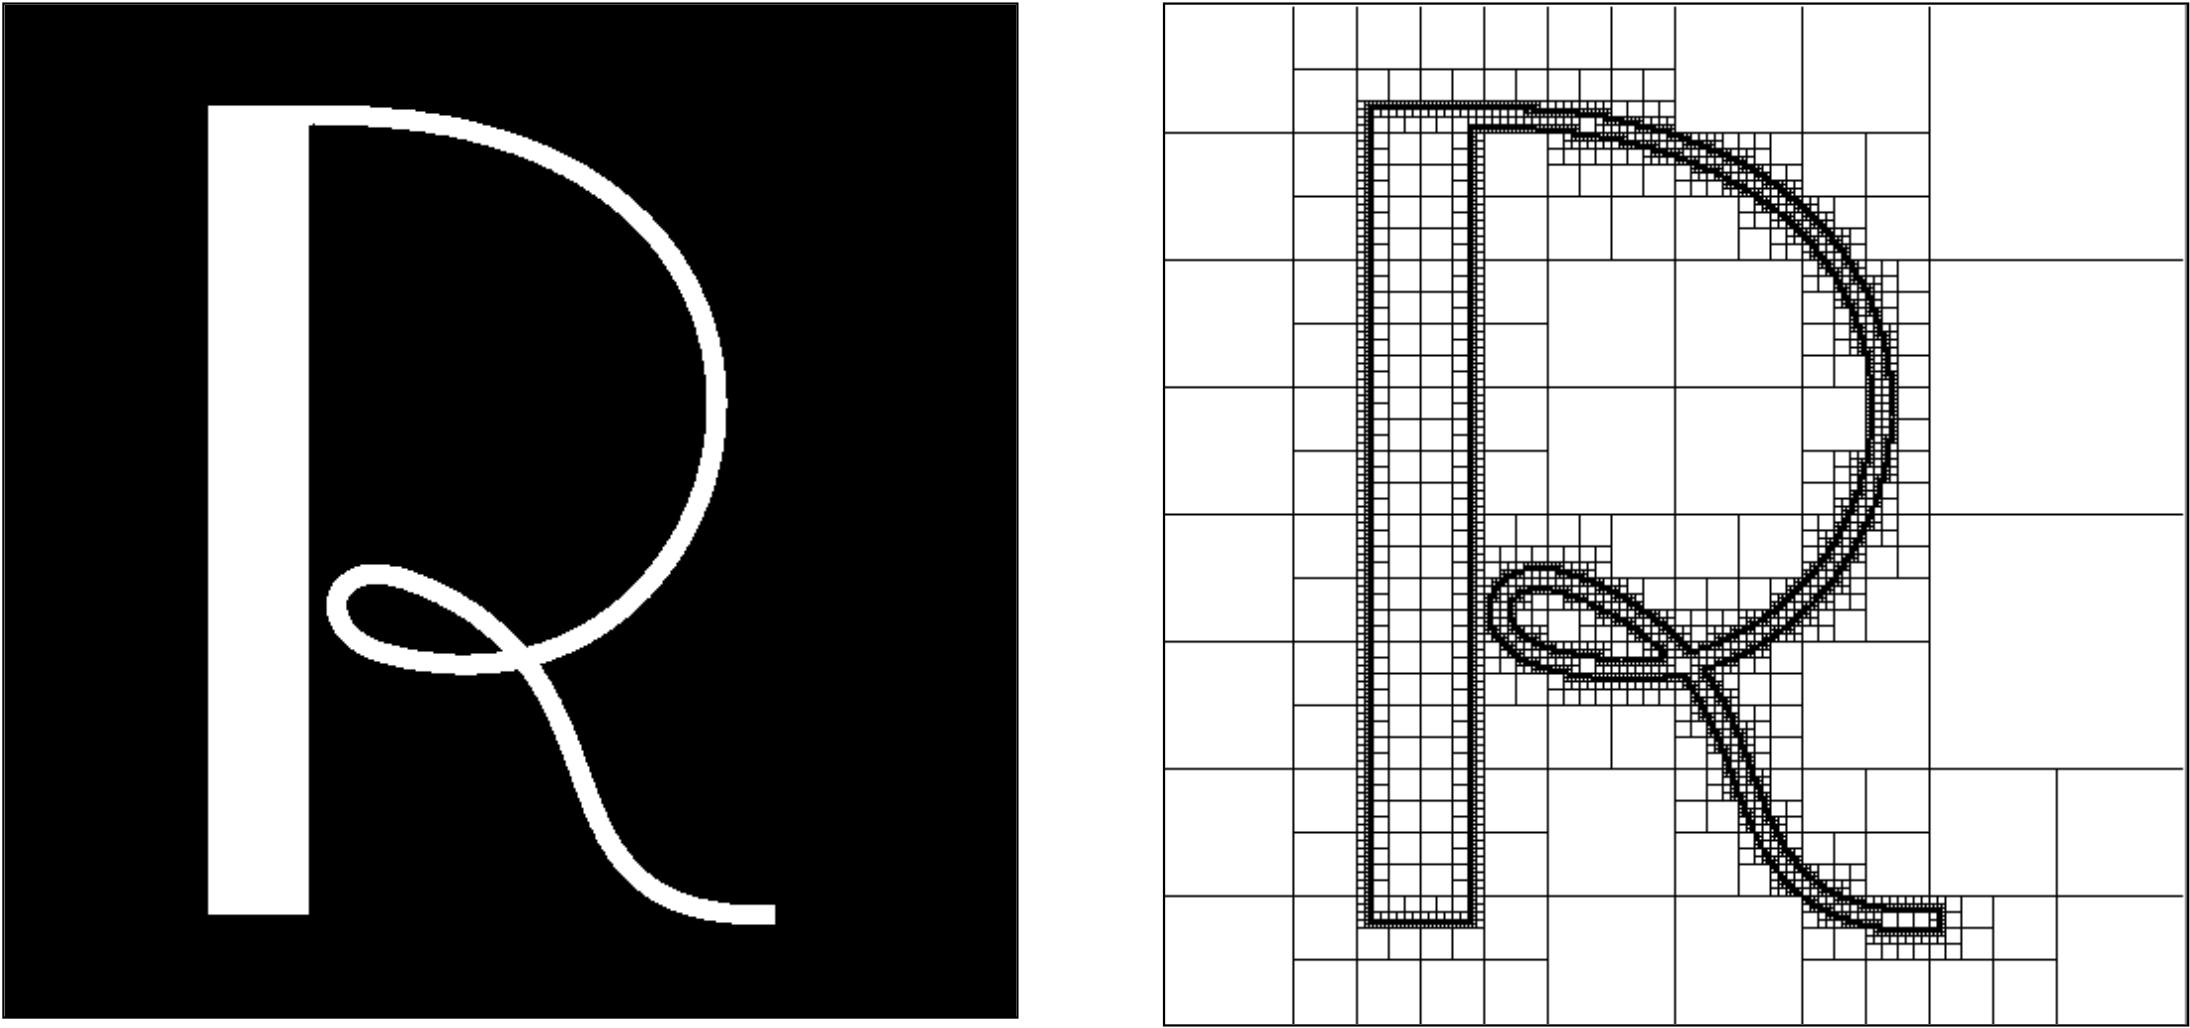
\includegraphics[width=\textwidth]{figures/df/adf-1}
		\caption{阶层式表述}
	\end{subfigure}
	\begin{subfigure}[b]{0.5\thewidth}
		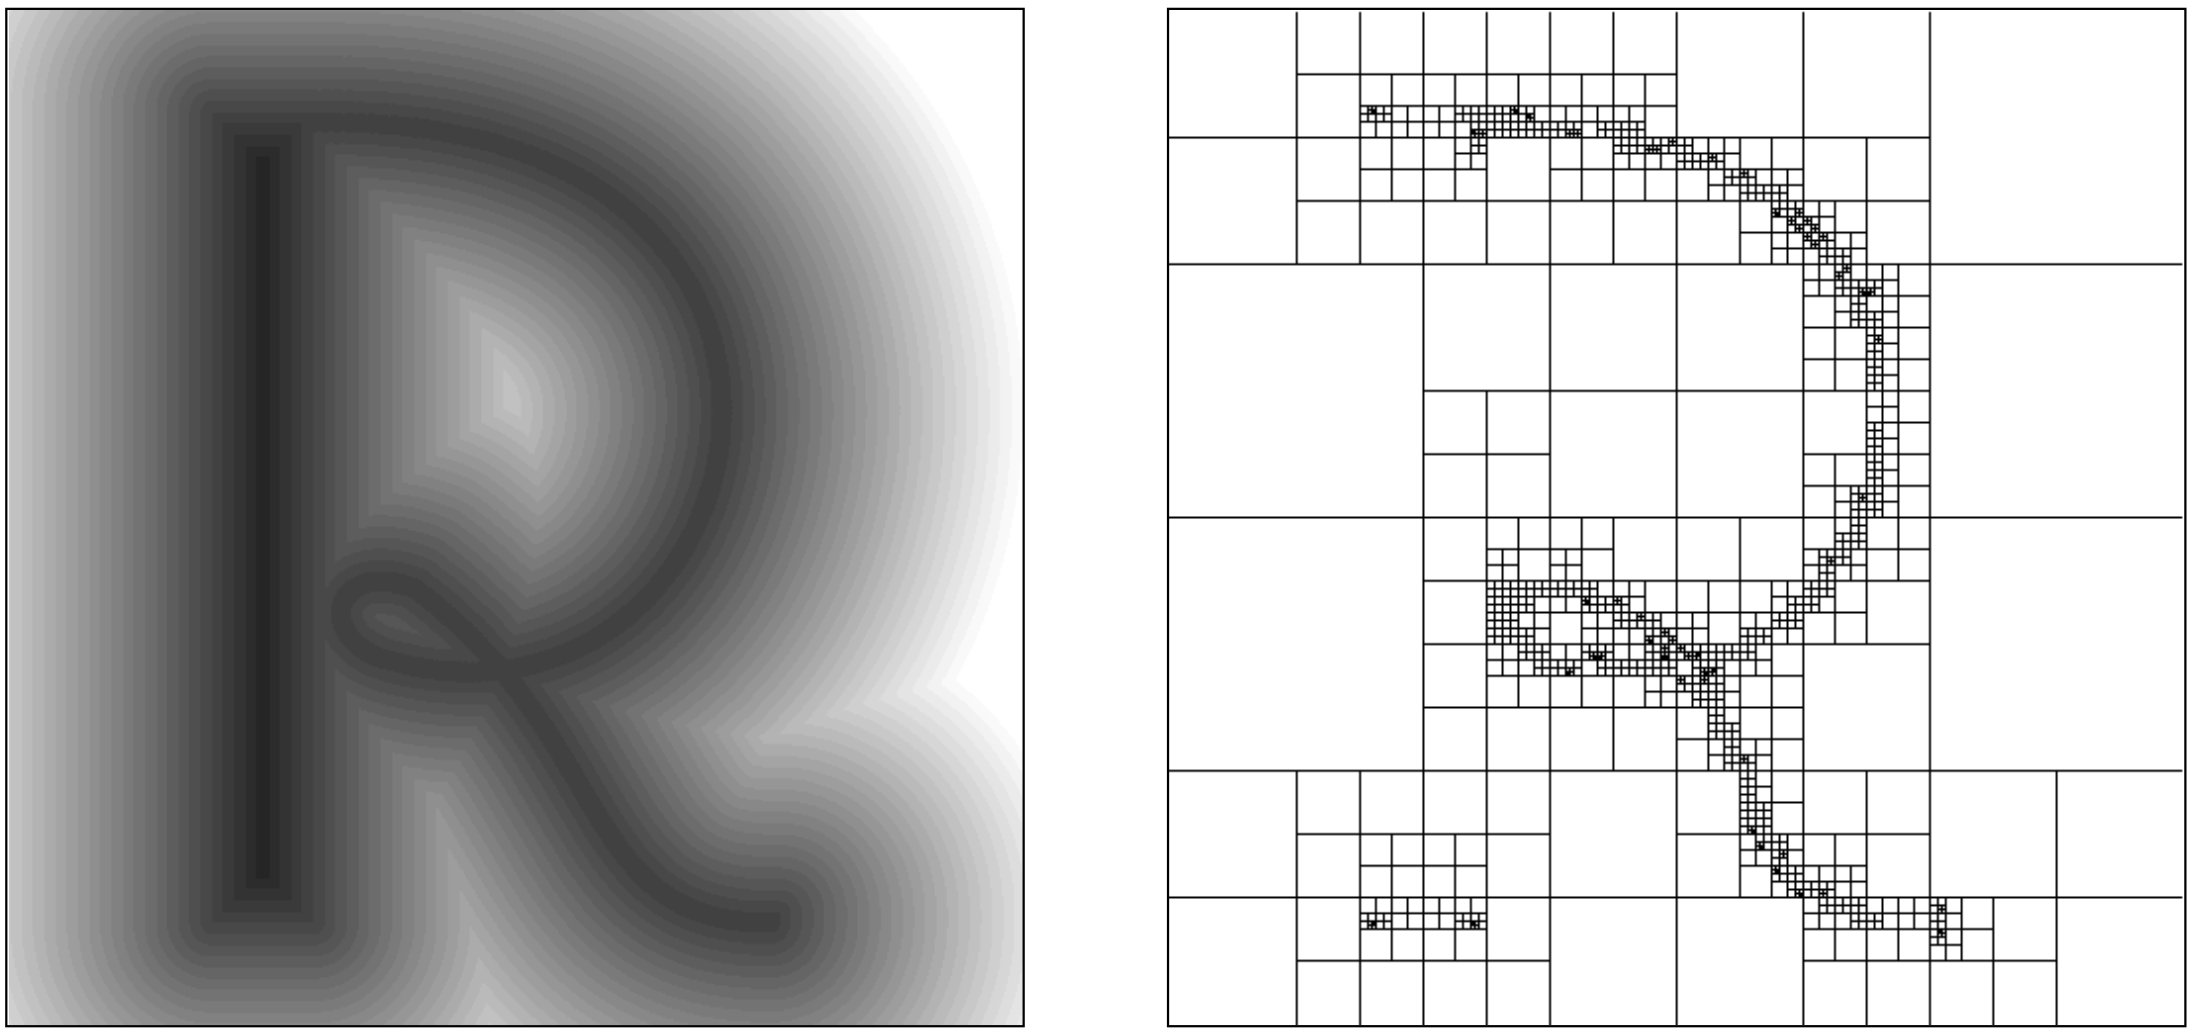
\includegraphics[width=\textwidth]{figures/df/adf-2}
		\caption{适应性表述}
	\end{subfigure}
	\caption{字形”P”的适应性距离场表述(b),可以看到只有物体曲面及边角的位置,其采样密度分布才会很密集,那些比较平面的区域则可以使用很稀疏的采样密度,而阶层式表述(a)在这些平面区域会使用占用更多的存储(图片来自\cite{a:adf})}
	\label{f:df-adf}
\end{fullwidth}
\end{figure}

给定图\ref{f:df-adf}中的一个形状,和传统的适应性方法类似,我们可以通过比较 当前单元与父级单元的平均距离差异来决定是否要对其进行细分,每个单元的 平均距离值可以通过对四个角的距离进行线性插值计算出来。

从图\ref{f:df-adf}也可以看出,即使是高度曲线化的边也可以很有效地使用适应性 距离场进行表述,因为线性插值可以很好的表述弯曲的边,那些较平滑的曲线 并不需要使用太多的阶层层级。但是那些边角或尖角等极度不平滑的位置附近 确实需要较多的阶层层级。

适应性距离场的生成需要使用到距离函数,这可以使用本章前面介绍的一些方法进行计算。

虽然适应性距离场的存储占用非常有效,但是它也具有一些缺点。由于使 用了适应性采样,因此那些较平坦的区域使用了较少的样本,造成这些区域的 过渡不平滑,这从图\ref{f:df-adf}最由小图中也可以看出,在“R”字形左边的一竖,由于形状 比较平坦,这造成了水平方向上并不能反映这一竖带来的高频率,因此我们可 能需要某种方向性信息,适应性距离场只有在弯曲的曲面部分才表现的足够好。 这种采样特征也会导致那些比较干净的区域出现一些斑点,如图\ref{f:ue4-adf-problem}(a)的天花板上的顶柱。这使得我们希望寻找一种更加平滑的方法。

\begin{figure}
\begin{fullwidth}
	\begin{subfigure}[b]{0.5\thewidth}
		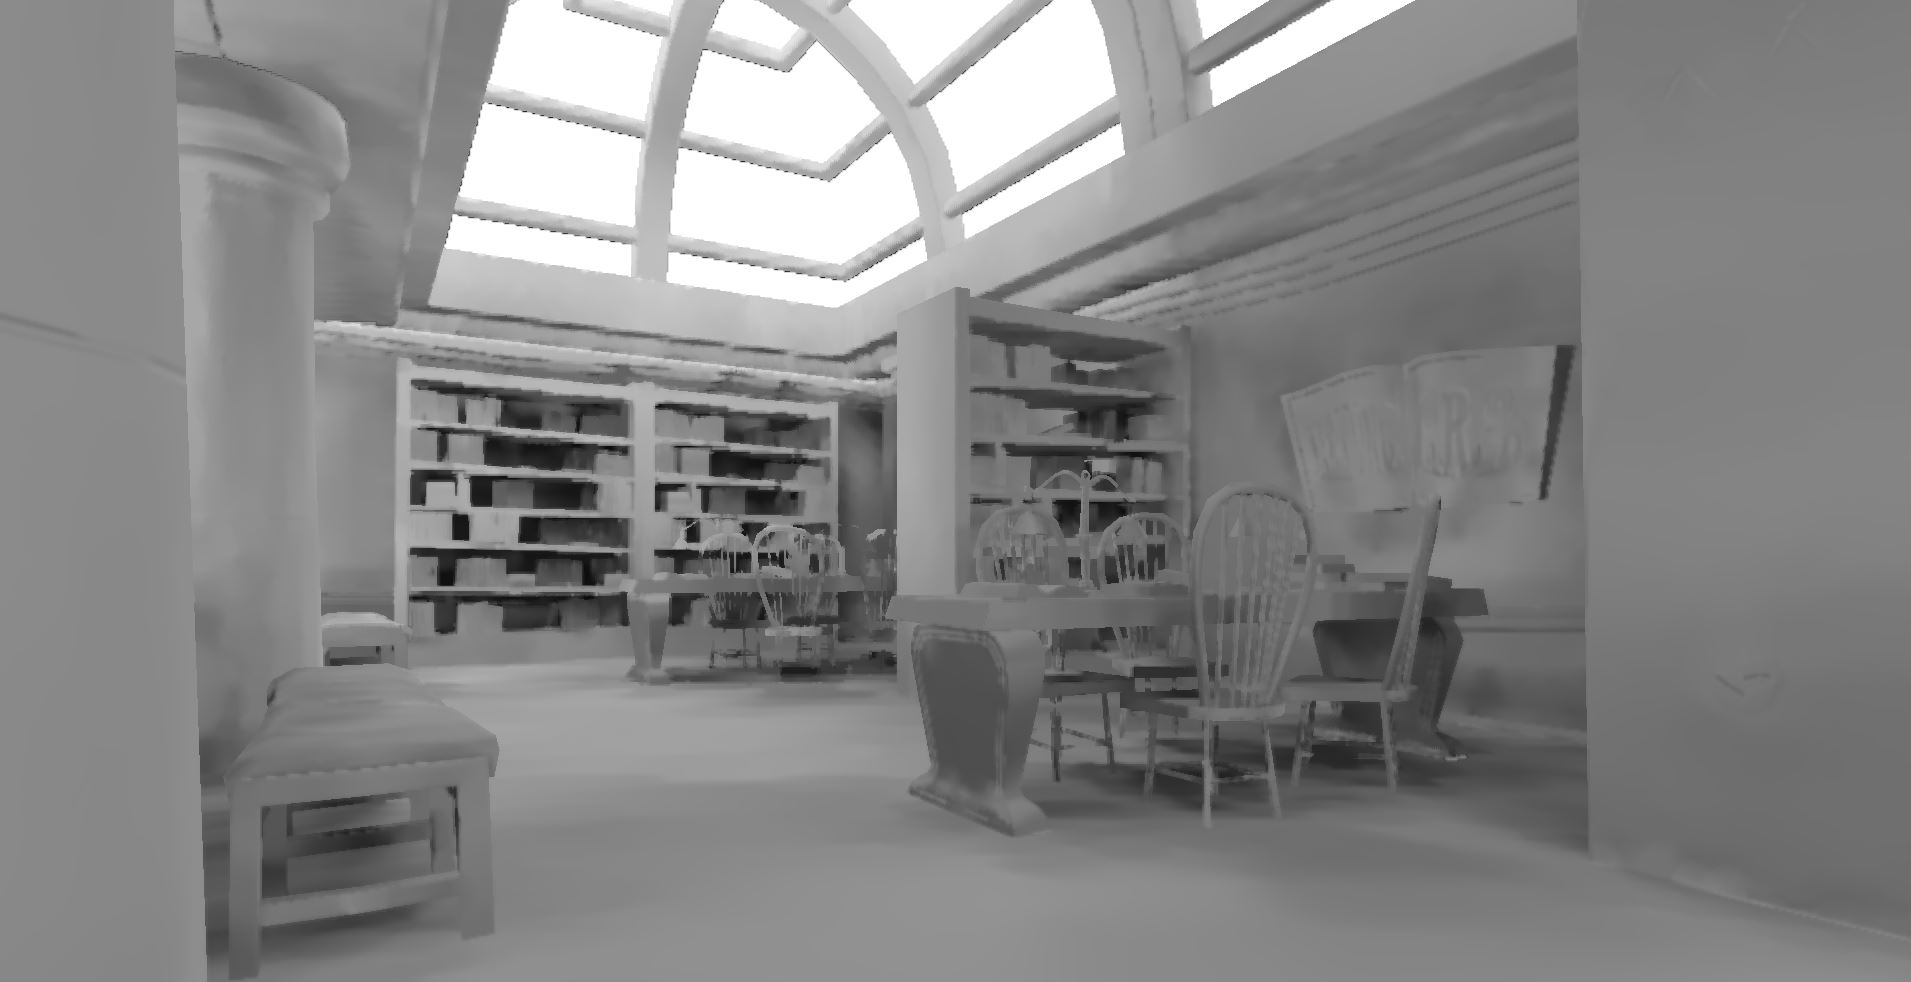
\includegraphics[width=\textwidth]{figures/df/DFAO_View_OldMethod}
		\caption{使用适应性距离场的AO}
	\end{subfigure}
	\begin{subfigure}[b]{0.5\thewidth}
		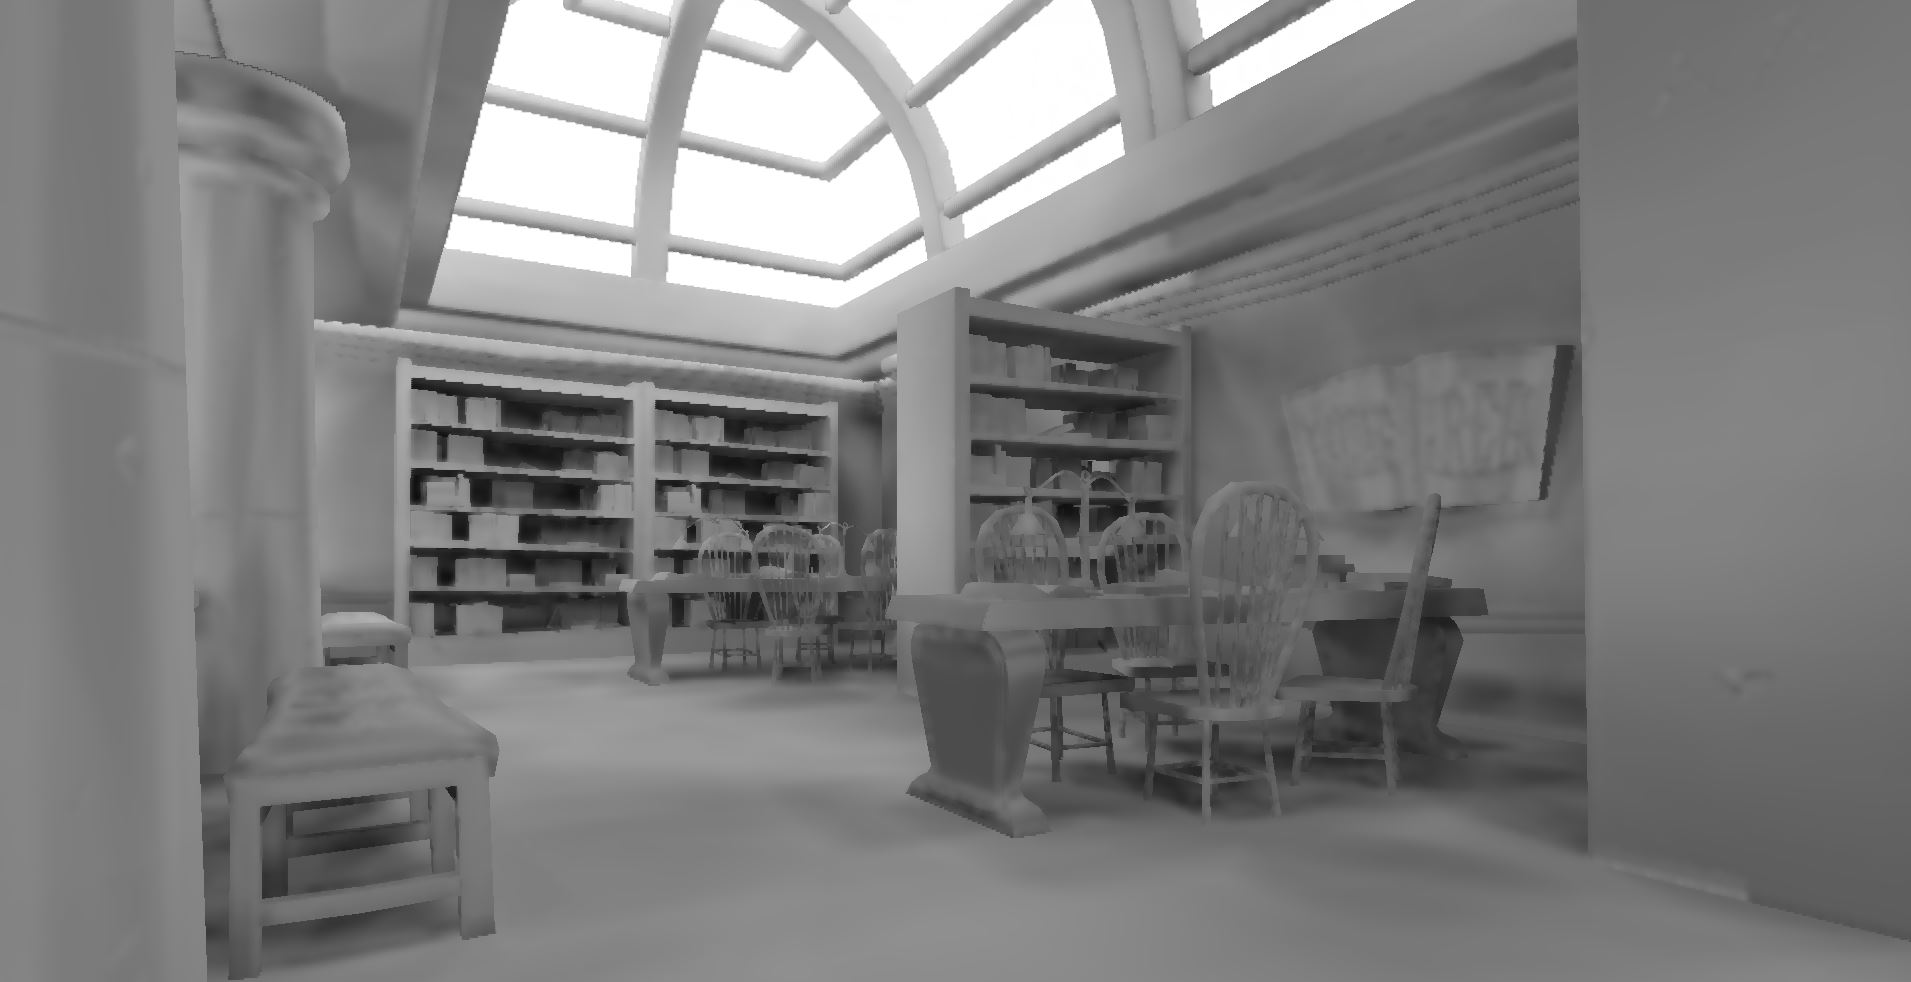
\includegraphics[width=\textwidth]{figures/df/DFAO_View_NewMethod}
		\caption{更平滑方法下的AO}
	\end{subfigure}
	\begin{subfigure}[b]{0.5\thewidth}
		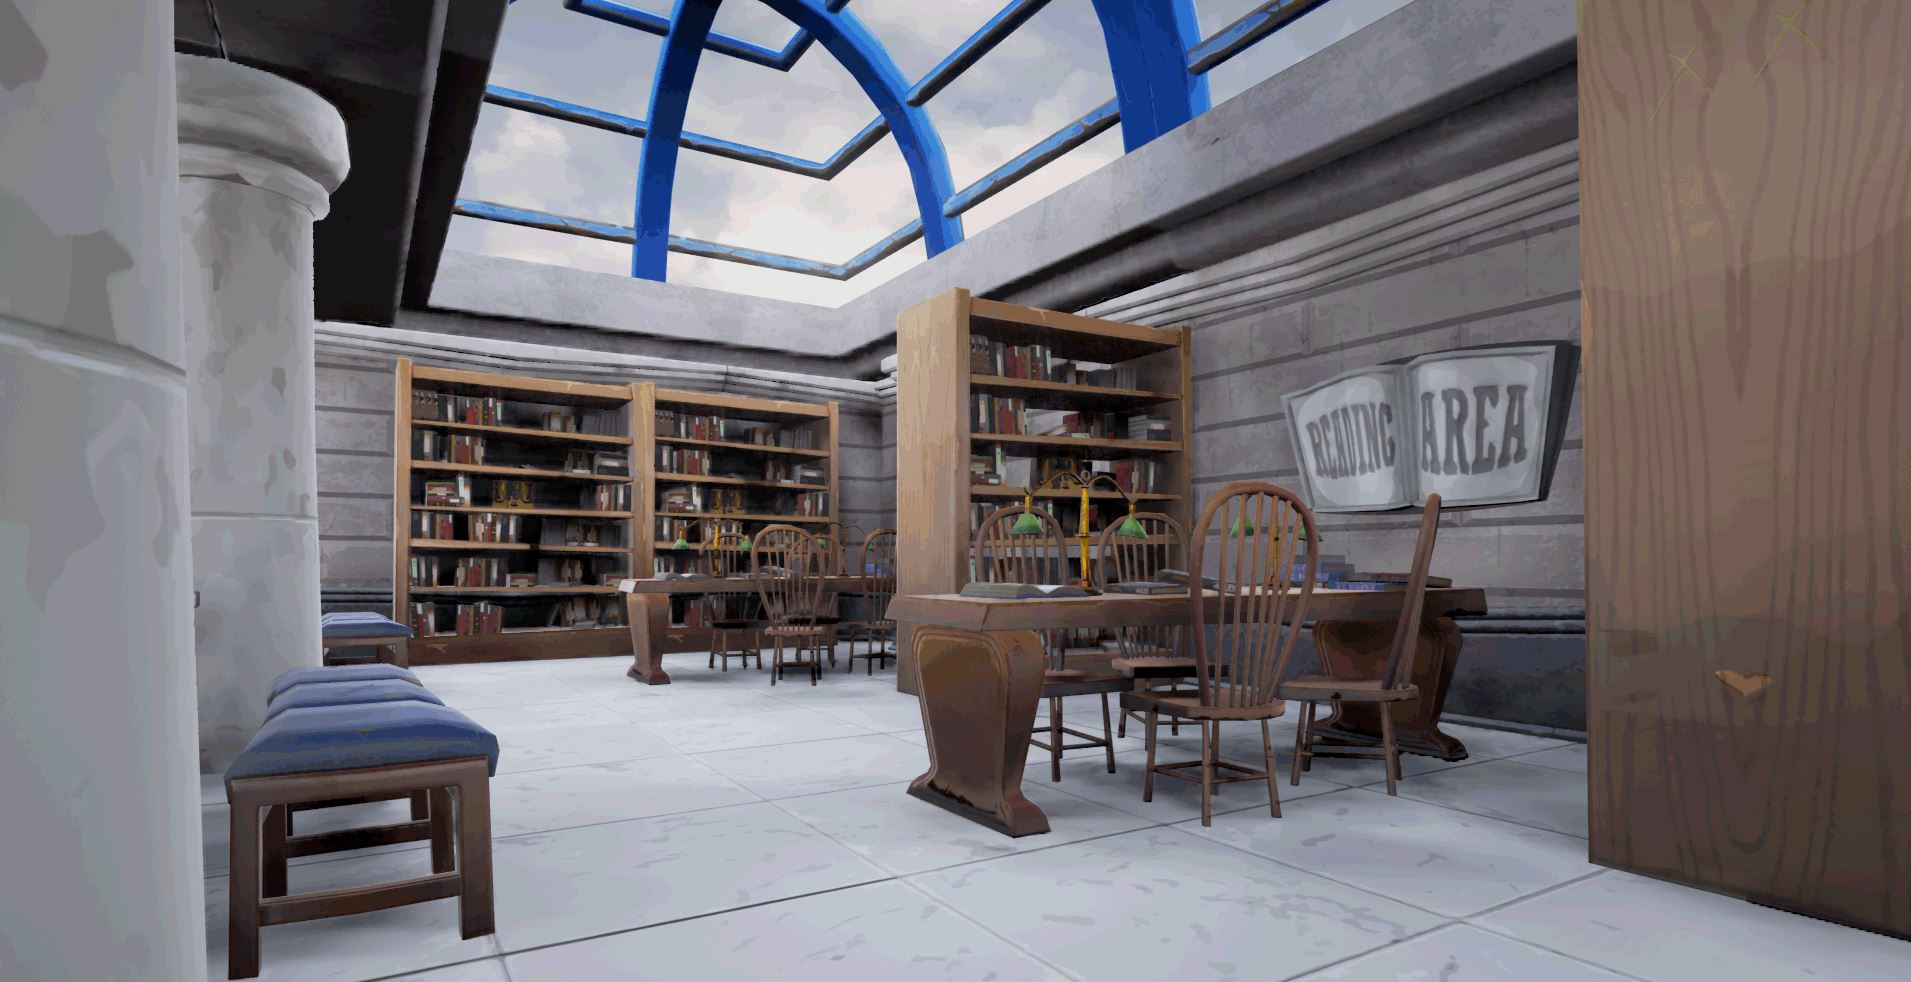
\includegraphics[width=\textwidth]{figures/df/DFAO_Scene_OldMethod}
		\caption{使用(a)渲染的结果}
	\end{subfigure}
	\begin{subfigure}[b]{0.5\thewidth}
		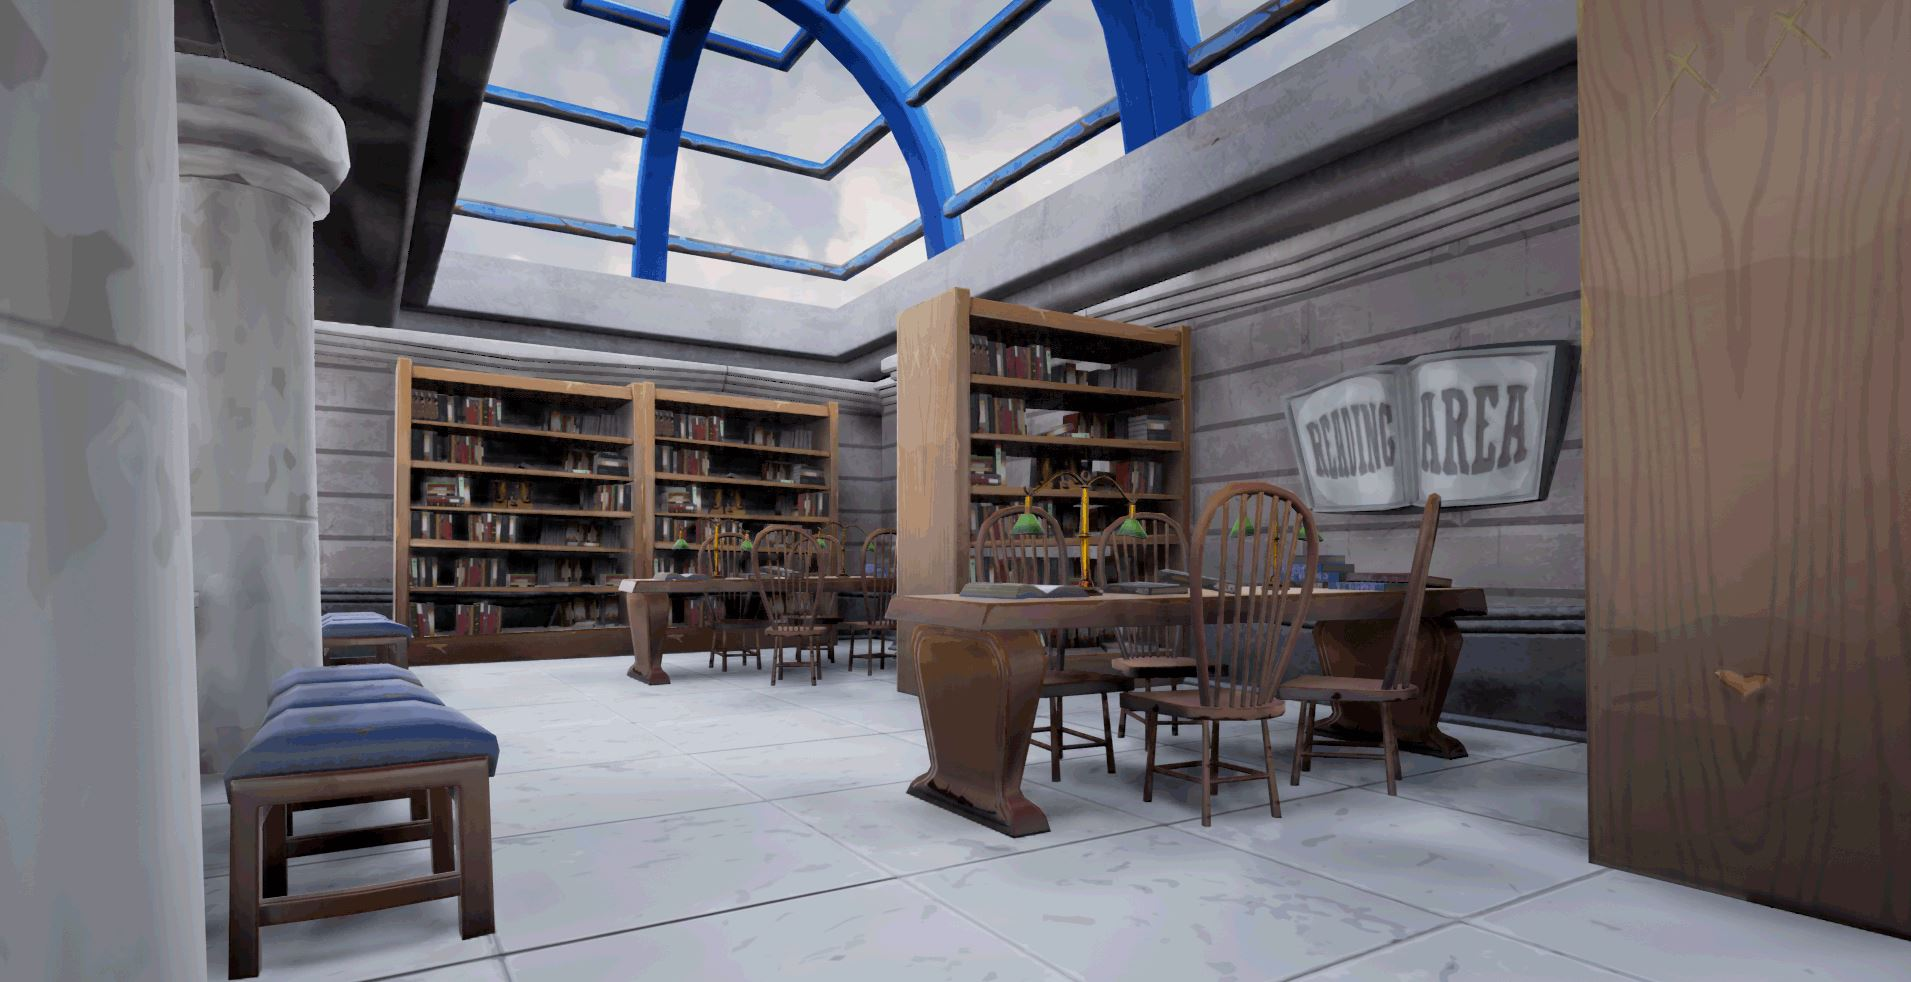
\includegraphics[width=\textwidth]{figures/df/DFAO_Scene_NewMethod}
		\caption{使用(b)渲染的结果}
	\end{subfigure}
	\caption{适应性距离场和其它一些更加平滑的方法的对比,在 Unreal Engine 4中,由于这种在平坦过度稀疏采样导致的问题,这种适应性采样已经被弃用(图片来自Epic Games)}
	\label{f:ue4-adf-problem}
\end{fullwidth}
\end{figure}




\subsubsection{完全距离场}
由于奈奎斯特采样定理(Nyquist’s sampling theory)\myindex{奈奎斯特采样定理}{Nyquist’s sampling theory}的限制,没有一种基于线性理论体积采样方法能够完全捕捉表面的细节,例如那些边角和棱边,这些区域的频率是无限的。完全距离场表述则完全不依赖于奈奎斯特定理采样定理,它构造出这样一个体积,其中每个体素拥有能够影响这个局部体积内距离值的表面的全部描述。

完全距离场表述(Complete distance field representation,CDFR)\myindex{完全距离场表述}{Complete distance field representation}\cite{a:A-Complete-Distance-Field-Representation}有一个完全的距离定义,这种定义完全区别于线性采样定理\footnote{如本书前面的内容可知,这又称为是基于点采样的方法,它们使用单个离散的值来表述一 段距离,就像在 GPU 的纹理中,其中每个纹素表示一个离散的颜色值,然后着色器通过对 这些纹素执行过滤操作来获取任意位置处的颜色值,因此基于点采样的距离场表述方法(例如前面介绍的适应性距离场)通过对相邻体素的距离值进行过滤来计算任意体素位置处的距离值,CDFR 则完全不依赖于过滤。但是CDFR可以被嵌入进适应性距离场表述中以提供 距离值的提取(而不是使用ADF本身的线性插值),这样能节省 CDFR 的存储和处理时间。},一旦距离体积被构建,我们便可以从中提出出任意精度要求下的任意距离等量线。

CDFR基于这样一些观察,例如,假设在一个1D空间,这里有一个脉冲(impulse)\myindex{脉冲}{impulse},因此这个地方的频率是无限的,由已知内容可知,我们是无法在不发生走样的情况下使用有限的采样频率对这个脉冲进行采样的。但是另一方面,这个脉冲的有符号距离函数确实一个线性函数,它从负的无穷延伸向正的无穷,如图\ref{f:df-1-dimension-space}右上小图所示,而这个线性函数却可以使用非常低的采样率得到非常精确的结果。

\begin{figure}
	\sidecaption
	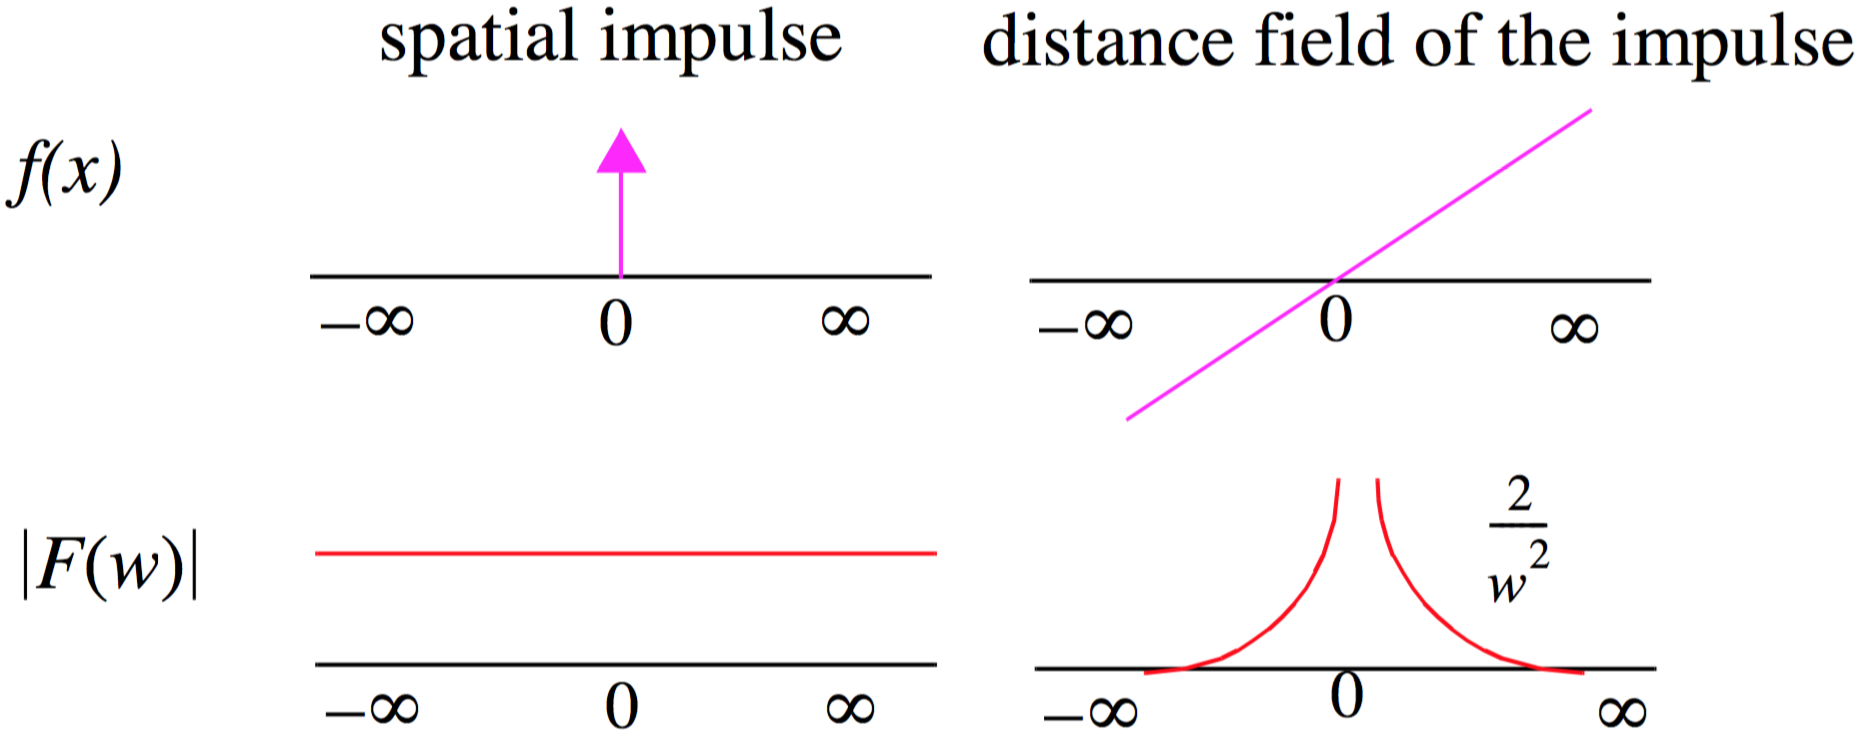
\includegraphics[width=0.65\textwidth]{figures/df/1-dimension-space}
	\caption{在不使用低通过 滤的情况下,我们不可能对 一个脉冲进行采样,但是我 们可以对这个脉冲的距离场 进行采样}
	\label{f:df-1-dimension-space}
\end{figure}

为了捕捉图\ref{f:df-1-dimension-space}中脉冲的准确位置,这里不需要使用采样,相反,我们需 要做的是在某个位置放置一个锚点,然后记录这个锚点到脉冲的有符号距离。 通过这种方法,脉冲的准确位置能够被很直观的表述,这个观察引出了一个新的关于距离场的表述。

一个完全距离定义(complete distance definition,CDD)\myindex{完全距离定义}{complete distance definition}是指一系列参数,这些参数同时描述一个 3D 位置到一个几何基元表面的的位置,以及这个几何 基元本身。特别地,当一个几何形状是使用三角形网格进行表述时,完全距离定义可以归纳为一个二元组,其中包含一个标准的标量距离值,以及一个关于三角形的描述,这个描述由一个三角形的顶点列表和边的列表构成,即:

\begin{equation}
	<distance,<v_1,v_2,v_3>,<e_1,e_2,e_3>>
\end{equation}

这里的距离值 $distance$ 是一个在欧几里得空间中由体素中心到一个三角 形的距离值,$< v_1,v_2,v_3 >$ 和 $< e_1,e_2,e_3 >$ 的值构成一个基础三角形(base triangle)\myindex{基础三角形}{base triangle},该基础三角形可以用于计算距离值 distance 的符号,这可以通过基 础三角形向外的法线方向和体素的相对位置 $pnt$ 来唯一确定。

对于一个三角形和一个3D的位置点 $pnt$,如果$pnt$正交地投影到C1区域,如图\ref{f:df-complete-distance-definition}所示,则该点的距离值等于点 $pnt$ 到三角形所在平面的距离,其符号可由 C1 的法线方向和投影方向的相对关系判断,此时 C1 即是点 $pnt$ 的 基础三角形;否则,如果 $pnt$ 正交地投影到任意一条边上,则其距离等于点 $pnt$ 到该边的最短距离,定义点 $pnt$ 在该边上的正交投影点为 $p^{'}$ ,同时定义矢量 $V$ 由 $p^{'}$ 指向 $pnt$,则在共享该边的两个三角形中,其向外法线\footnote{所谓向外法线,是指对于三角形的每条边,其垂直于该边并指向三角形外部的一个矢量。}方向更接近$ V$ 的 三角形为点 $pnt$ 的基础三角形,这可以通过比较点积 $|v \cdot Normal|$ 来确定;对于C3 情形,其距离为点 $pnt$ 到最近的顶点的距离,在共享该顶点的多个三角 形中,我们可以使用和 C2 类似的方法确定点 $pnt$ 基础三角形,这通过比较所 有共享该顶点的三角形的向外法线与 $V$ 的接近度来决定。

\begin{figure}
	\sidecaption
	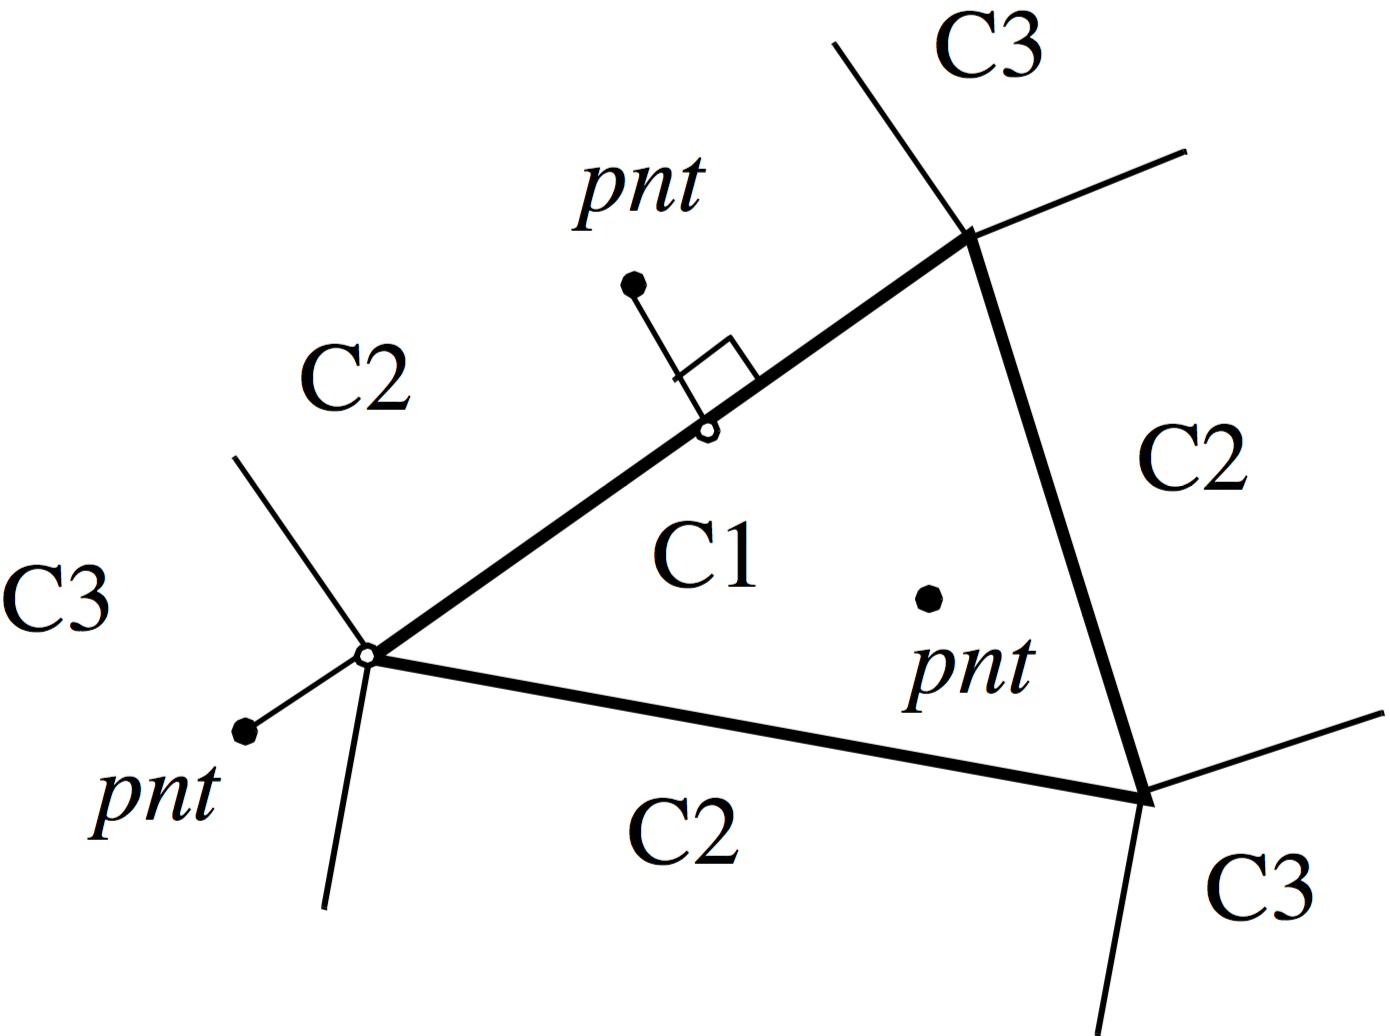
\includegraphics[width=0.35\textwidth]{figures/df/complete-distance-definition}
	\caption{如果$pnt$投影到三角形内部,其结果为C1,否则根据其投影点是靠近一条边还是一个顶点,其结果为C2或者C3,注意为了简便这里只画出了2D的情形}
	\label{f:df-complete-distance-definition}
\end{figure}

有了上述方法描述,我们便可以构建一个完全距离场表述,它允许以任意 精确度准确捕捉所有的几何细节。给定一个表面网格,在体素化阶段,我们对每个体素存储一个完全距离定义,而不是单个距离值。




\section{隐式表面的渲染}\label{sec:df-rendering-of-implicit}
通过前面的知识,我们已经知道了什么是隐式表面,以及怎样表述它,现 在我们将要讨论怎样渲染一个隐式表面。尽管从后面的内容可知,我们的主要 目标其实并不是使用场景的隐式表述来进行渲染,而是借助距离场这种隐式表 述来计算可见性相关的信息,例如环境遮挡和软阴影等,但是距离场表述的渲 染和可见性计算的基础工具是一样的,这就是球体追踪,所以本节首先从渲染 的角度来学习距离场的球体追踪。

但是在开始介绍球体追踪之前,我们首先来总结一下几种一般的场景表述 方法以及这些表述方法所使用的渲染技术,因为太过比较解决同一问题的两种 不同的方案,通常能够让我们更好地理解这两种方案的本质。

在本节,我们首先会总结一些关于光栅化和光线追踪的概念,然后介绍常 用的体积渲染技术,并由此引入对于距离场表述的渲染技术,即球体追踪,最 后介绍一些球体追踪的改进方法。




\subsection{表面表述与渲染}
如本书前面的内容所述,在当前工业中,绘制 3D 场景主要有两种方法,即 光栅化和光线追踪,尽管本书前面已经介绍了很多关于它们的知识,但是本节 还是先对它们做一个总结和比较,然后我们会明白,为什么在这两种基础渲染 架构后面,另外一种特殊的基于距离场的渲染是有价值的。

光栅化和光线追踪通常都使用相同的场景表述方式,如本章前面第\ref{sec:df-parametric-surface}节关于参数化表面表述的内容可知,一个参数化的表述在$R^{n−1}$作用域内定义表面的每一个点,在计算机图形学中,我们通常使用一个由一些三角形组成的网 格来表述场景,其中这些三角形的顶点将表面离散成多个平面片段。在渲染的 时候,CPU 会将这些包含顶点,顶点索引及法线等信息的数据发送至 GPU,然 后 GPU 将对这些顶点执行光栅化以向着色器提供表面上每个像素的位置,然 后着色器利用每个像素的信息对其进行着色计算。通常这里可以使用高洛德着色(Gouraud shading)\myindex{高洛德着色}{Gouraud shading}模型,这种方法只对网格的每个三角形顶点执行着色计算,然后对三角形内部的像素执行线性插值,另一种更好的方法是冯氏着色(Phong shading)\myindex{冯氏着色}{Phong shading}模型, 这种方法在光栅化阶段只对法线执行插值计算,然后在像素着色器中使用这个插值计算的法线以及相关的反射模型计算每个像素的颜色。这两种方法在 3D 着色领域拥有相当长的历史,即使在今天,这些模型仍然被使用,只是增加了一些基于物理的效果。

上述的方法称为光栅化(rasterization)\myindex{光栅化}{rasterization},它具有一些优点,例如高度并行 化计算,相对 CPU 更简化但更高效的内存模型,相关的内容可以参见本书前面第2章的内容,现代图形处理器都被优化以更好地支持光栅化管线。但是它也有一些很严重的缺点,例如它不支持间接光照,并且其性能几乎跟三角形和光 源的数量呈线性关系。因此,一些其它辅助技术被引入以解决这些问题,例如 间接光照缓存,环境贴图,阴影图等。这些辅助技术使得渲染的图像更加真实, 然而它们通常大都依赖于一些预计算,因此无法适用于动态场景,我们需要另 外一些能够更真实的,并以一种更自然的方式模型光照传输的方法。

能实现这个目标且最重要的方法显然是光线追踪(ray tracing)\myindex{光线追踪}{ray tracing},最早的光 线追踪算法只从摄像机经过每个屏幕像素向场景发出一条光线,直到该光线击中场景的某个表面而停止,光线不再继续追踪。

光线追踪算法的下一个发展来自于\cite{a:Animprovedilluminationmodelforshadeddisplay},在该方法中,当一个 光线击中一个表面时,它会同时产生三条不同类型的新的光线,即反射光线,散 射光线和阴影光线。反射光线(reflection ray)从原始光线的镜面反射方向发 射,场景中与其相交的最近的一个物体表面即是反射光线看到的结果;散射光 线穿入进半透明的物体内部,不同的是散射光线可能穿过物体或者从入射点附 近散射回到表面外部;阴影光线则是向所有光源发射,如果在光源和表面之间 遇到任何不透明物体,则该表面被阴影遮挡,该阴影光照的贡献为0。这种递归的光线追踪算法大大提升了渲染图像的真实度。

对于表面上的每个点,由于像素尺寸远远大于微观尺寸,因此光线会从多个方向反射,这方面的理论知识可以参见本书第\ref{chp:intro}章的内容。因此理论上我们需要对每个点发射多条反射光线,反射光线以及阴影光线,这样为了达到更好的结果,每个点需要发射上百条新光线,一直递归下去,每个像素可能需要额外上千的光线数量,这对于即使是离线渲染其成本也是非常高的。所以光线追踪算法通常采用蒙特卡洛方法来解决光照传输的积分问题。

在光线追踪算法中,其最困难的部分在于光线-表面的相交计算。在一个显式表面表述中,对于每条光线的相交计算,我们必须遍历场景中的每一个三角 形。为了加速相交计算,一些阶层式的空间细分数据结构被采用,例如八叉树,kd树等。然而即使使用这些加速的数据结构,这个计算过程耗时仍然十分严重。

为了避免光线-表面相交计算,一种方法是直接定义整个3D场景中的每一个点,这将我们引向场景的体素表述(voxel representation)\myindex{体素表述}{voxel representation},如图\ref{f:df-Voxelgitter}所示, 每个物体被离散化为一个体素表格(voxel grid)\myindex{体素表格}{voxel grid}。由于场景中整个 3D空间中的每一个点都被表述,因此一条光线可以直接执行相交测试,不需要迭代其它物体,离散的体素之间的点可以使用双线性插值或其它GPU支持的过滤技术计算而出,这种将一个物体表示成离散体素的过程称为体素化(voxelization)\myindex{体素化}{voxelization}。

\begin{figure}
	\sidecaption
	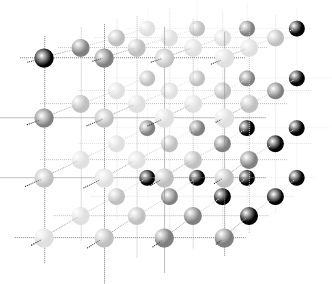
\includegraphics[width=0.35\textwidth]{figures/df/Voxelgitter}
	\caption{一个体素表格的示意图,这里每个体素都包含一个颜色值(图片来自于Wikipedia)}
	\label{f:df-Voxelgitter}
\end{figure}

在体素表述中,常使用的渲染技术是光线步进,我们将在下一节讨论,体 素模型通常是一种显式的表面表述技术,即每个体素会直接存储表面信息,例 如颜色,法线分布等,上一章讨论的基于体素的全局光照技术使用的正是这种 结构。




\subsection{光线步进}
传统上,一个物体被模型化为一个具有无限薄边界的表面,然后通常一个平面化的纹理被映射到这个表面上,这个纹理可能是程序生成的,或者从现实 世界采样,它可能包含颜色等信息,也可能是包含位置位移信息,通过这些额 外的数据来描述表面的方式通常称为表面的参数化。

但是,许多物体的表面定义非常复杂,以至于很难使用上述这种表面模型, 例如毛皮,织物等材质;另一些物体,例如被那些侵蚀的材质或流体,这些物 体往往拥有一些比较复杂的边界,例如可能这些边界是人工雕刻的,其使用体素的表述会更加合适;还有一些物体,如火焰,云和烟雾,它们甚至没有一个 能够很好定义的边界表面。

\cite{a:hypetrtexture}发现许多物体的表面可以直接使用一个函数进行描述,这个函数定义于 $R^{3}$ 的某部分子区域,为此,他们使用了一种称为超纹理(hypertexture)\myindex{超纹理}{hypertexture}的概念定义了一个介于物体与空白空间的中间区域,这个区域通常可以通过控制函数来实现动态调整,如图\ref{f:df-hypetrtexture}所示。

\begin{figure}
	\begin{subfigure}[b]{0.33\textwidth}
		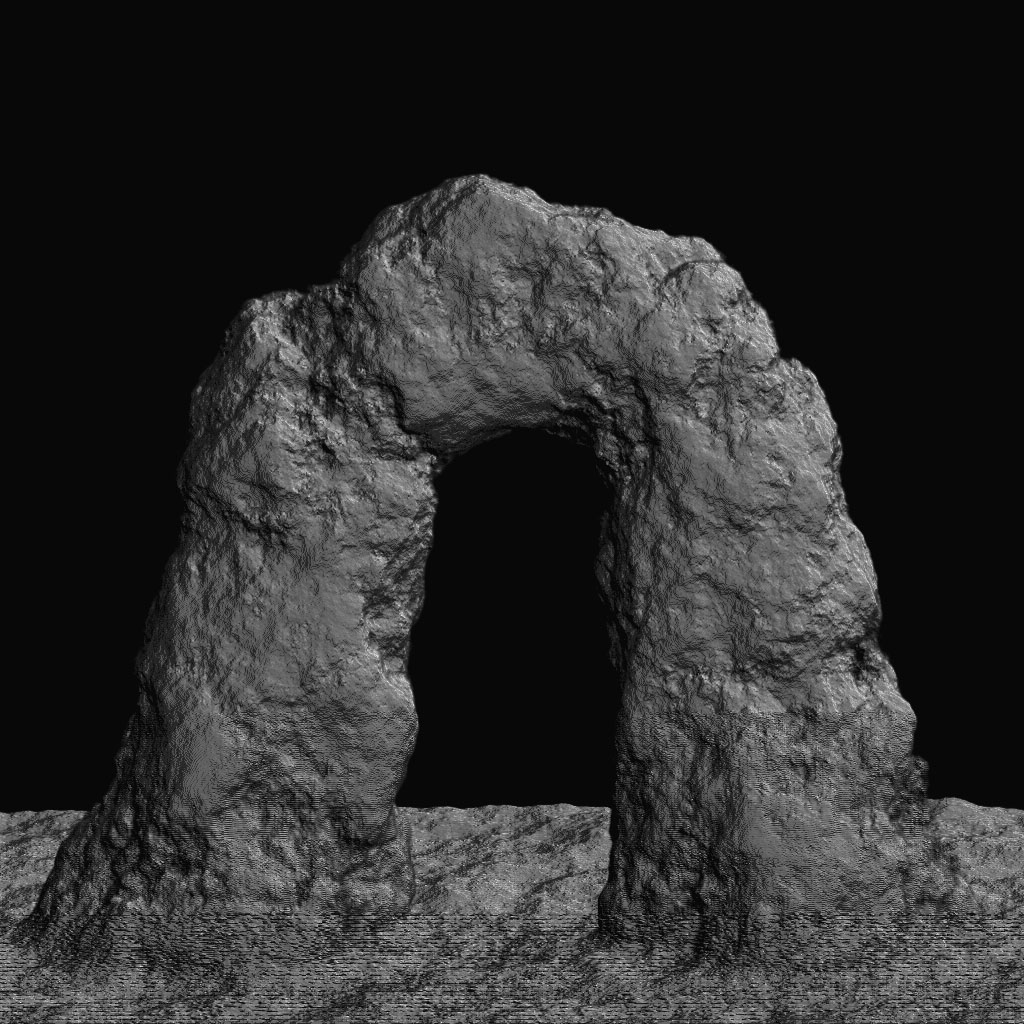
\includegraphics[width=\textwidth]{figures/df/hypertexture1}
	\end{subfigure}
	\begin{subfigure}[b]{0.33\textwidth}
		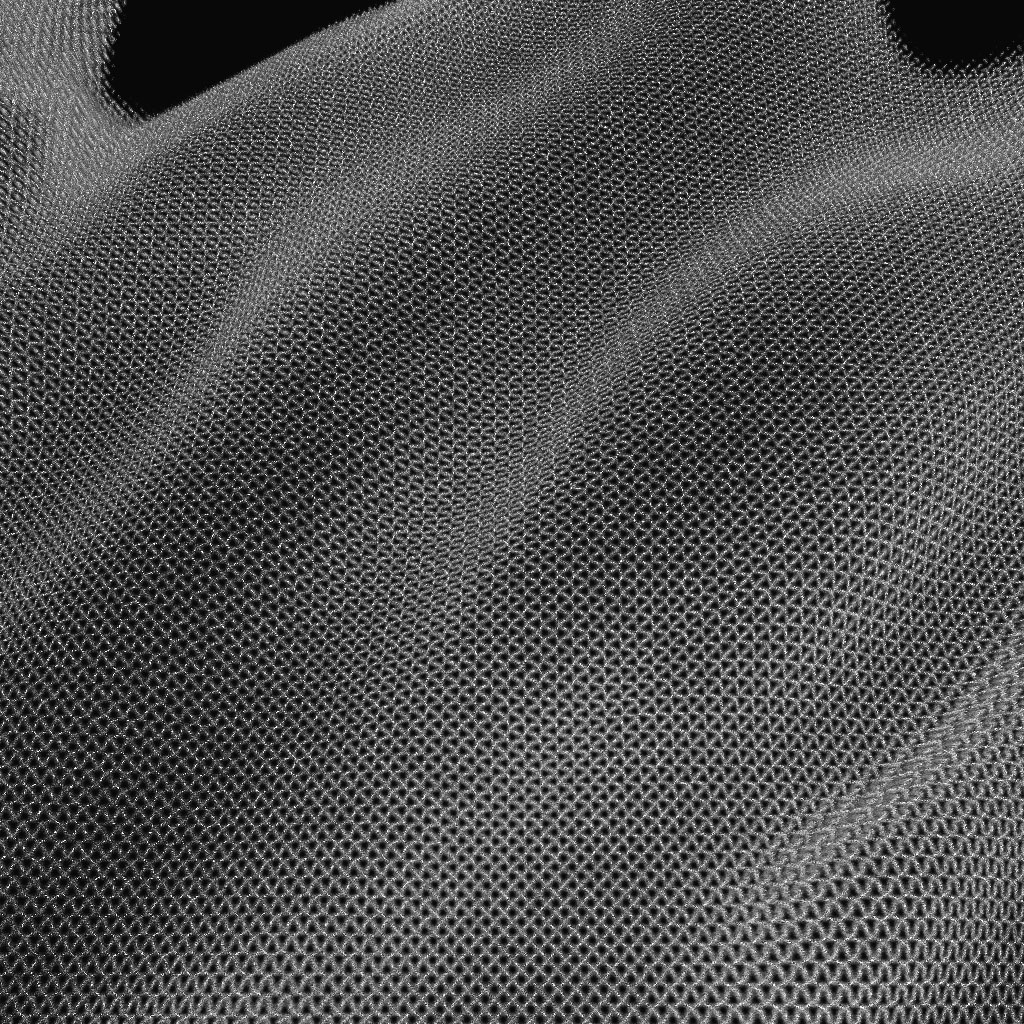
\includegraphics[width=\textwidth]{figures/df/hypertexture2}
	\end{subfigure}
	\begin{subfigure}[b]{0.33\textwidth}
		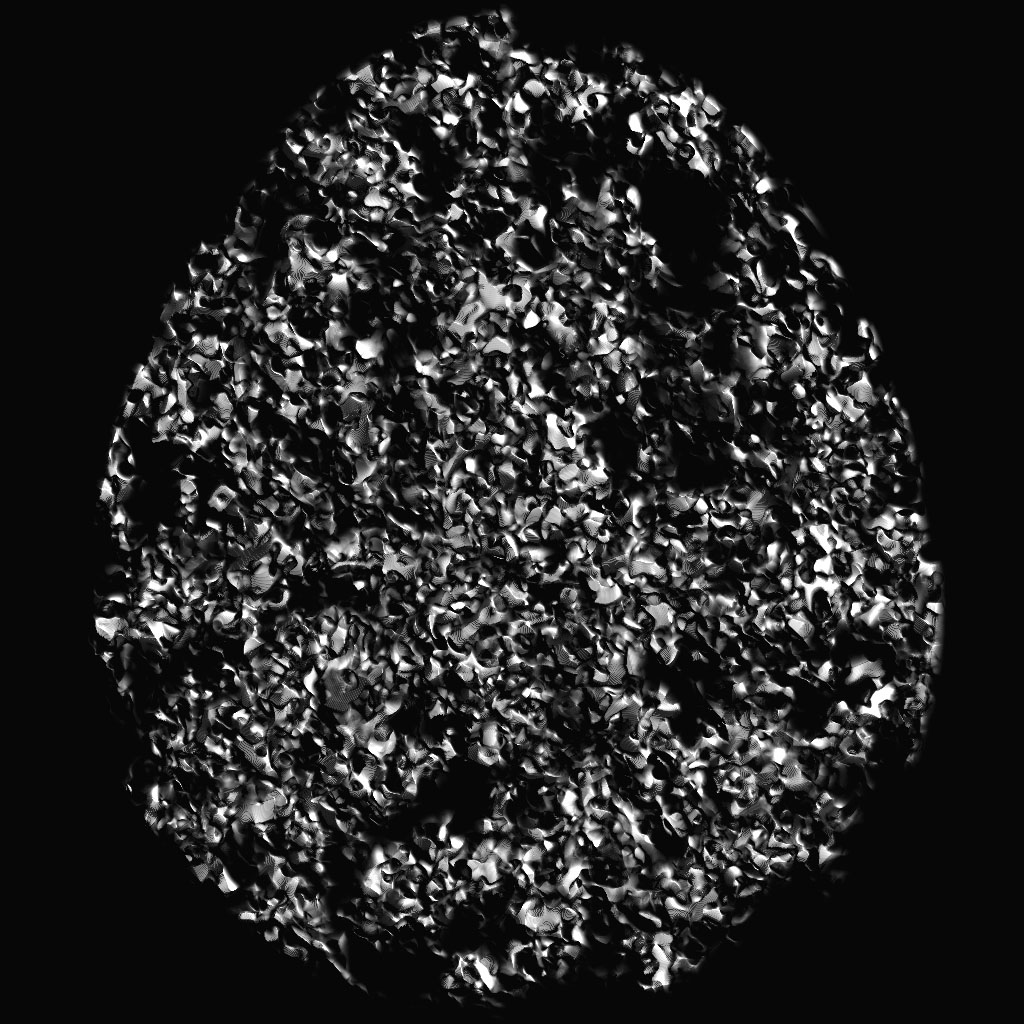
\includegraphics[width=\textwidth]{figures/df/hypertexture3}
	\end{subfigure}
	\caption{一些复杂物体的表面可以使用超纹理进行表述(图片来自\cite{a:hypetrtexture})}
	\label{f:df-hypetrtexture}
\end{figure}

超纹理使用了下述概念:

\begin{itemize}
	\item 物体密度函数(object density function)\myindex{物体密度函数}{object density function}$D(x)$,其取值范围为 $[0,1]$,它描述 的是在 $R^{3}$ 空间内一个形状内所有点 $x$ 处的密度值,其中物体的表面定义了 一个软区域(soft region)\myindex{软区域}{soft region},在该区域内的取值为 $0 < D(x) < 1$。
	\item 密度调整函数(density modulation function,DMF)\myindex{密度调整函数}{density modulation function}$f_i$, 该函数用于调整软区域内物体的密度,每个密度调整函数用于控制物体空间特征的某一个层面,所有的密度调制函数就构成了一个体积造型的工具集。
\end{itemize}

超纹理通过连续地对一个物体的物体密度函数 $D(x)$ 作用一系列密度调制函数$f_i$来创建,即:

\begin{equation}
	H(D(x),x)=f_n(\cdots f_2(f_0(D(x))))
\end{equation}

形式上,一个软物体(soft object)\myindex{软物体}{soft object}是指定义在 $R^{3}$ 上的一个密度函数 $D(x)$, 其值在物体内部为 1.0,在物体外部为 0.0,而其软区域 $0.0 < D < 1.0$ 是一个 具有一定厚度的薄层,它介于物体内部和外部之间。

因为超纹理是一个 $R^{3}$ 上的体积表述,所以它常常没有定义良好的表面,它常常使用体积渲染相关的技术进行渲染,即光线步进算法。

\begin{figure}
	\sidecaption
	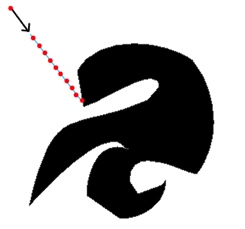
\includegraphics[width=0.35\textwidth]{figures/df/ray-marching}
	\caption{光线步进算法使 用一个常数增量沿光线方向 离散采样,以寻找光线与表面的交点}
	\label{f:df-ray-marching}
\end{figure}

在传统的光线步进(ray marching)\myindex{光线步进}{ray marching}算法中,每个像素向模型空间投射一条 光线,然后该光线与一个包含超纹理体积的平行六面体执行相交测试,这可以 使用例如\cite{a:Onraytracingparametricsurfaces}提供的方法,如果光线与某个平行六面体相交,其分别 代表该光线进入与离开该平行六面体位置的光线参数 $\mu_0$和 $\mu_1$ 首先被计算,然后光线步进从光线参数值 $\mu_0$ 开始,以一个固定的增量 $\Delta\mu$ 步进,对光线步进 过程中的每个点进行采样计算(如图\ref{f:df-ray-marching}所示):

\begin{equation}
	x=x_{\mu_0}+k\Delta x_{\mu}
\end{equation}

这里 $k = 0, 1, 2, ...$,并且 $\mu_0 + k\Delta\mu\leq \mu_1$,$\Delta x \mu$ 是沿光线步进过程中的位移增量。下面是光线步进的伪代码:

\begin{lstlisting}[language=C++, mathescape=true]
$k=0$
$d=0$
while $k < k_{\rm max}$ do
	$d=f(r(k))$
	if d≤0 then return $k\Delta t$
	$k=k+1$ return 0
\end{lstlisting}

需要注意的是,光线步进算法具有一些问题,如图\ref{f:df-ray-marching-problems}所示,如果步进的 增量太大,则很可能光线很可能传入物体内部很大的距离,因此其对物体表面 形状的辨识精确度大大降低。不仅如此,光线步进甚至可能漏掉整个或者部分表面。所以光线步进的增量应该尽可能地小,以便更好地估计表面的边界。

\begin{figure}
	\sidecaption
	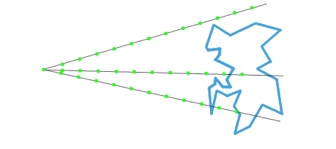
\includegraphics[width=0.65\textwidth]{figures/df/ray-marching-problems}
	\caption{物体的表面使用蓝色的轮廓线表示,绿色点表示光线步进的采样点,这些采样点之间的距离由步进步幅决定}
	\label{f:df-ray-marching-problems}
\end{figure}

后面将看到,上述的问题可以被距离场表述很好地解决,这也是光 线步进和球体追踪的区别所在,同时这也是一般的体素表述与隐式表面表述的区别。




\subsection{球体追踪}
不像一般的光线追踪,球体追踪算法主要聚焦于寻找第一个光线与场景表面的交点,这避免了在光线追踪中遍历整个场景的高昂计算。

在距离场中的每一个点,如果围绕该点画一个球体,并且使用该点的距离 值作为半径,则这可以保证在该球体空间范围内不存在任何物体,这个体积在\cite{a:Ray-Tracing-Deterministic-3-DFractals}中被称为未包围体积(unbounding volume)\myindex{未包围体积}{unbounding volume},因此我们可以 使用这个半径作为光线步进的增量,因此这样的光线步进具有一个可变的步进 增量。如果持续按照这样的方式沿光线步进,则我们可以最终找到一个该光线 与某个表面的交点,这样的过程可以从图\ref{f:df-sphere_tracing}中看出,我们称这样的技术为球体追踪(sphere tracing)\myindex{球体追踪}{sphere tracing}。

\begin{figure}
	\sidecaption
	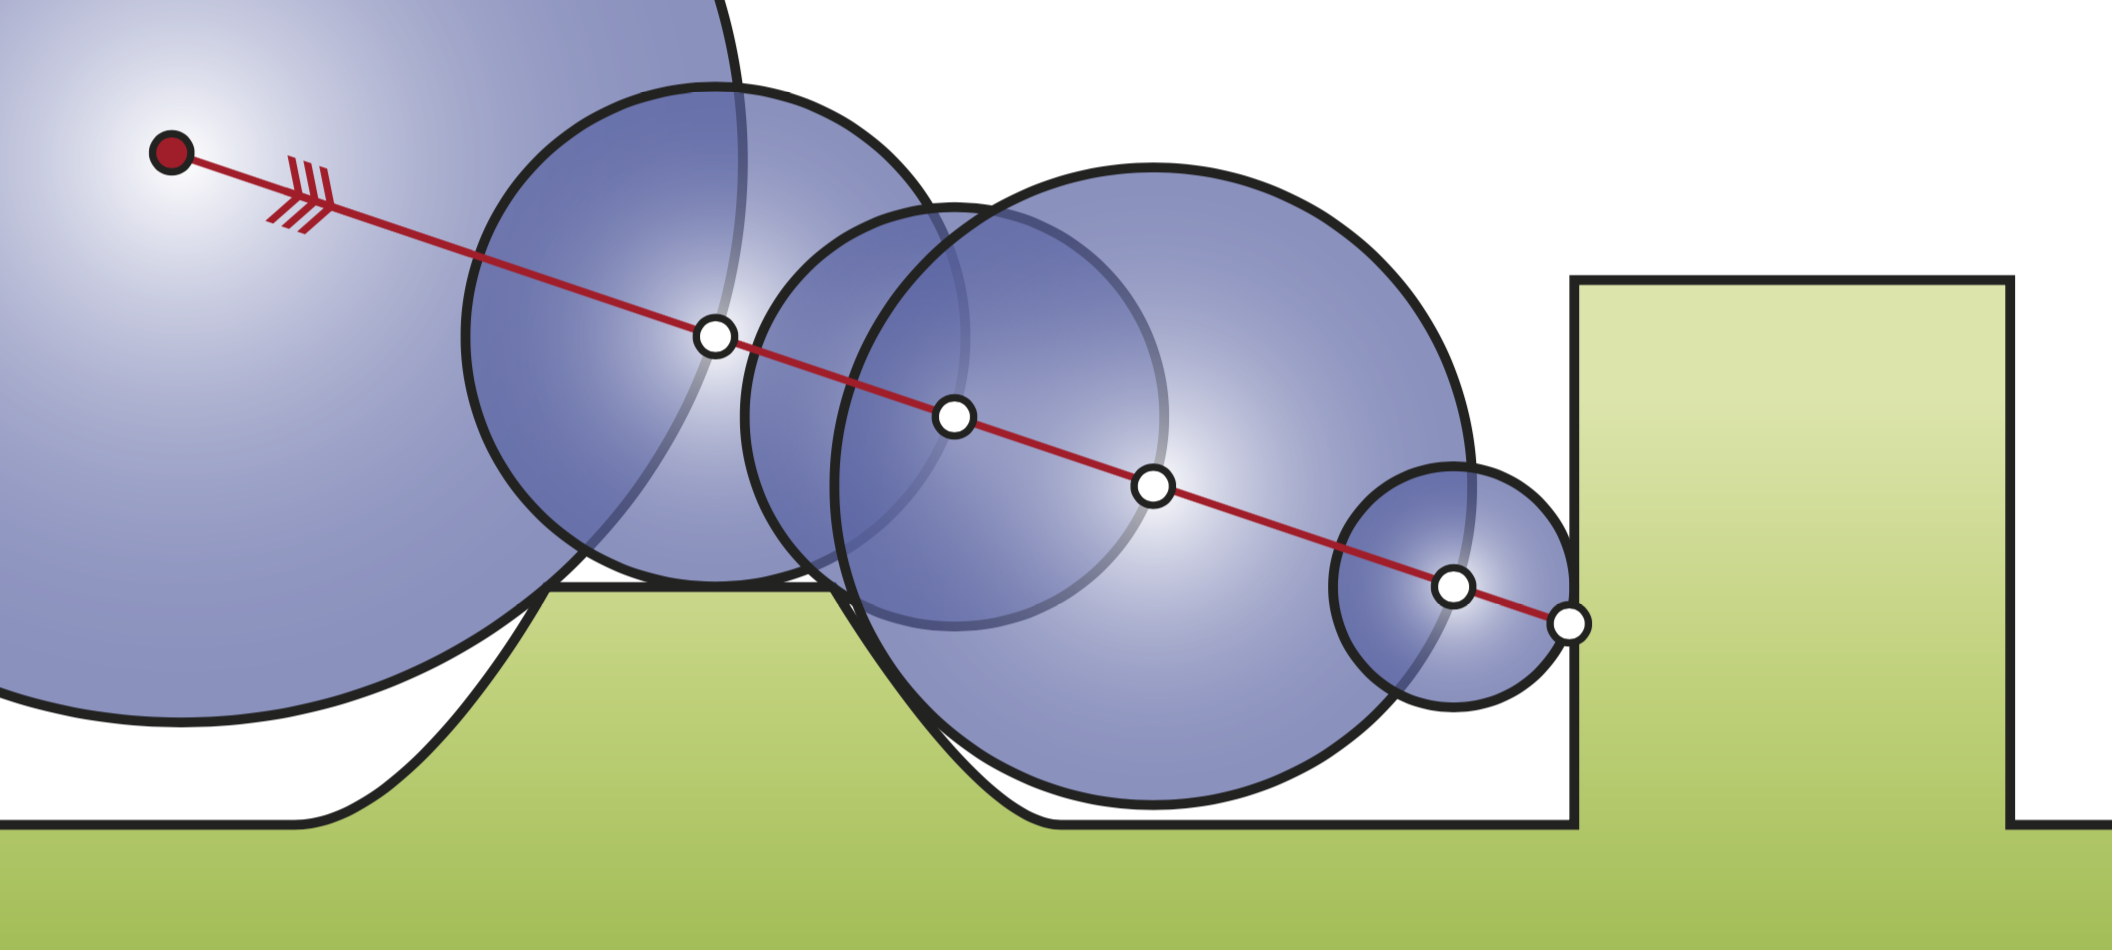
\includegraphics[width=0.65\textwidth]{figures/df/sphere_tracing}
	\caption{在球体追踪中,每个步进增量由其体素的距 离值动态决定,光线持续步进直到距离值小于某个阈值 或者击中一个表面(图片来自\cite{a:Enhanced-Sphere-Tracing})}
	\label{f:df-sphere_tracing}
\end{figure}

为了结束球体追踪的过程,我们使用一个光线可以穿越的最大距离(即所有步进累积的长度)$D$,以及一个最小的距离阈值 $\epsilon$,这通常是一个很小的数 字,它表示我们希望收敛的一个精度,球体追踪的伪代码如算法如下所示:

\begin{lstlisting}[language=C++, mathescape=true]
$k=0$
$d=0$
	while $t < D$ do
	$d = f(r(t))$
	if $d\leq \epsilon$ then return $t$
	$t=t+d$ return 0
\end{lstlisting}

通过使用隐式表面表述,这提供了一个快速的光线追踪计算方法,我们可 以借助这种能力来实现一些全局光照效果,例如环境光照和软阴影,这也是本 章我们的主要目的,这些应用将在本章后面深入讨论。

需要注意的是,通过使用距离场表述,每个体素记录的不再是一个颜色值, 而是一个从该体素到最近表面的距离值,这就意味着我们不能直接使用球体追 踪来渲染表面,球体追踪只是帮助我们快速地找到光线追踪过程中第一个最近 交点的位置,为了取得该交点所在的表面位置,并通过该表面位置获取材质信 息以对该表面点进行着色计算,我们还需要使用传统的光线追踪来找到这个表 面点,但只不过此时不再需要对整个场景进行遍历,而只需要根据交点位置快 速定位到附近的一些物体,然后针对少量或者单个物体执行相交计算。当然本 章的重点并不是使用距离场来渲染表面,而且从后面的内容可以看到,对环境 遮挡等计算并不要求找到真正的表面相交位置。

从这里也可以看出本章的距离场与上一章介绍的体素表述的差别,虽然同 属体积表述,但上一章的体素直接记录了表面材质信息,因此可以直接通过这 种体素结构来渲染场景,那里的体素表述成了原始三角形网格表述的代理。而 本章的距离场只记录一个距离值,不包含任何材质信息,例如颜色值,这两种 不同的表述导致了两种完全不同的渲染方法。



\subsection{增强的球体追踪}
如果整个场景的距离场使用单个体积纹理存储,那么光线的每一次步进都 只是一个纹理采样操作,我们从采样的纹素中得到下一次步进的距离值,并将此距离值和最大和最小阈值进行比较,这样的步进过程就会很快。

但是前面已经讨论过,为了节约内存,我们应该使用一些阶层式的数据结 构来存储距离场,例如适应性距离场方法就使用一个八叉树来表述场景。在这 些阶层式的方法中,只有单个物体本身(即八叉树的一个叶节点)存储为一个 比较小的分辨率较高的体积纹理,而多个或全部物体被组合以形成分辨率更低 的阶层式距离场,如图\ref{f:df-DF_GlobalDF}右半部分所示。

\begin{figure}
	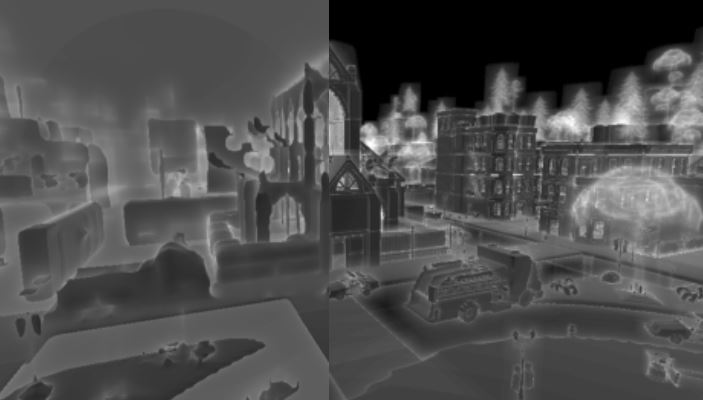
\includegraphics[width=\textwidth]{figures/df/DF_GlobalDF}
	\caption{Unreal Engine 4中场景的距离场可视化图像,右图中每个物体对应一个距离场,只有场景中的物体才会被计算,并且只记录很短的距离,那些空白空间则被忽略;左图则是一个全局的距离场,全局距离场的体素分布很稀疏,它主要用于让光线在空白空间步进时更高效(图片来自Unreal Engine 4官方文档)。}
	\label{f:df-DF_GlobalDF}
\end{figure}

当光线步进远离物体表面时,或者当光线进入一个大面积空白区域时,此 时的步进增量应该非常大,以提高步进效率。上述的距离场通常只对单个物体 产生,并且出于内存占用的考量,这些每物体距离场的最大距离范围会非常小, 如图\ref{f:df-DF_GlobalDF}右半部分所示,那光线进入那些不包含距离场的空间该怎样选择步进增量 呢?一些解决方案使用一些包围盒来标记这些空白空间,而在 Unreal Engine 4 中,除了对每个物体产生一个每物体距离场,引擎还会使用所有这些距离场来 生成一个全局距离场,这个全局距离场的分辨率很低,它可以使用前面介绍的 如距离变换等近似方法生成,因为它的主要目的是表述那些空白空间的距离分 布,当光线在场景中步进时,如果步进采样点距离表面很近,则那些每物体的 距离场被使用,如果采样点距离表面很远,则全局距离场被使用,这大大的加 速了球体追踪的效率,全局距离场的可视化效果如图 \ref{f:df-DF_GlobalDF}左半部分所示。

上述的方法是通过对距离场表述的改进来提高球体追踪的效率,下面我们将要介绍一些在算法层面的改进来提升球体追踪的效率,减少步进的时间。



\subsubsection{超松弛球体追踪}
在迭代法\footnote{参见本书前面第\ref{chp:rad}章第\ref{sec:r-iteration}节的内容。}(iterative method)\mathindex{迭代法}{iterative method}中,连续超松弛方法(successive overrelaxation method,SOR)\mathindex{连续超松弛方法}{successive overrelaxation method}\cite{a:Successiveoverrelaxationmethod} [Black and Moore, ] 是一种解决线性方程组 $Ax = b$ 的方 法,该方法从高斯-赛德尔方法(Gauss-Seidel method)外推\footnote{所谓外推法,它就是超出原始观察范围的一个估计的过程,这种方法用于加速计算时间,但 是其产生的结果具有不确定性,甚至可能是无意义的结果。}(extrapolation) 出来,这种外推方法对前一次迭代的结果和当前高斯-赛德尔迭代迭代结果之间 做一个加权平均,即:

\begin{equation}
	x^{(k)}_i=\omega\vec{x}^{(k)}_i+(1-\omega)x^{(k-1)}_i
\end{equation}

这里 $\vec{x}$ 表示原始的高斯-赛德尔迭代,而 $x$ 表示这里使用连续超松弛法得 到的最终迭代结果,$\omega$ 称为一个外推因子(relaxation factor)\myindex{外推因子}{relaxation factor}或者外推参数 (relaxation parameter)\myindex{外推参数 }{relaxation parameter},其背后的思路是选取一个外推因子 $\omega$ 的值使其能够 加速迭代向方程组的解收敛的速度,如果 $\omega = 1$,则上述的方法回归到高斯-赛 德尔方法本身,\cite{a:Gauss-seidelmethodsofsolvinglargesystemsoflinearequations}的一个定理指出,当 $\omega$ 的值位于区间 $(0, 2)$ 之外时,这种超松弛外推方法的收敛将会失败。 

需要注意的是,尽管外推方法本身会导致不相关的结果,但是超松弛外推方法本身是能够收敛到正确结果的,这是因为高斯-赛德尔迭代法本身能够收敛 到正确结果,超松弛外推法只是加速了这种收敛速度,因为每次迭代的近似结 果通常是单调递增或递减的,这样在少数出现错误的地方会被高斯-赛德尔方法 本身纠正,而那些大部分单调的地方则其收敛速度会被加速。

\cite{a:Enhanced-Sphere-Tracing}将这种超松弛法的原理运用到了球体追踪中,与原始的球体追踪算法使用每个位置处的距离值作为步进增量不同的是,这里使用 $\delta_i = f(p_i) \cdot \omega$ 作为新的步进增量,其中 $f(p_i)$ 表示第 $i$ 次迭代的位置处的距离 值,$\omega \in [1; 2)$ 为外推参数。

特别需要注意的是,这里只是借鉴了超松弛法的思路而已,球体追踪并不 是一个线性方程组,所以这并不是超松弛方法的一种应用。这里将光线的每个 步进“视作”超松弛方法中的一个迭代,其能够借用超松弛方法背后的原理,是 和超松弛方法使用的一个基本观察是一致的,即球体追踪中所有步进增量的函 数在某些(尤其是空白)空间是一个单调递增或单调递减函数,因此我们可以 使用类似超松弛方法的机制来加大步进的增量,以加速球体最终的速度。这种单调性可以从图\ref{f:df-over-relaxation}上面小图中看出,其左边的 7 次步进增量几乎都是单调递增 的,然后在右边表面的频率变化较大时,这种单调性发生改变,这也是超松弛 方法失效的地方,但是相对于单次失效,左边较大的区域内得到了很大的加速, 例如图\ref{f:df-over-relaxation}上面小图的 7 次迭代缩减为下图中的 4 次迭代。

\begin{figure}
\sidecaption
	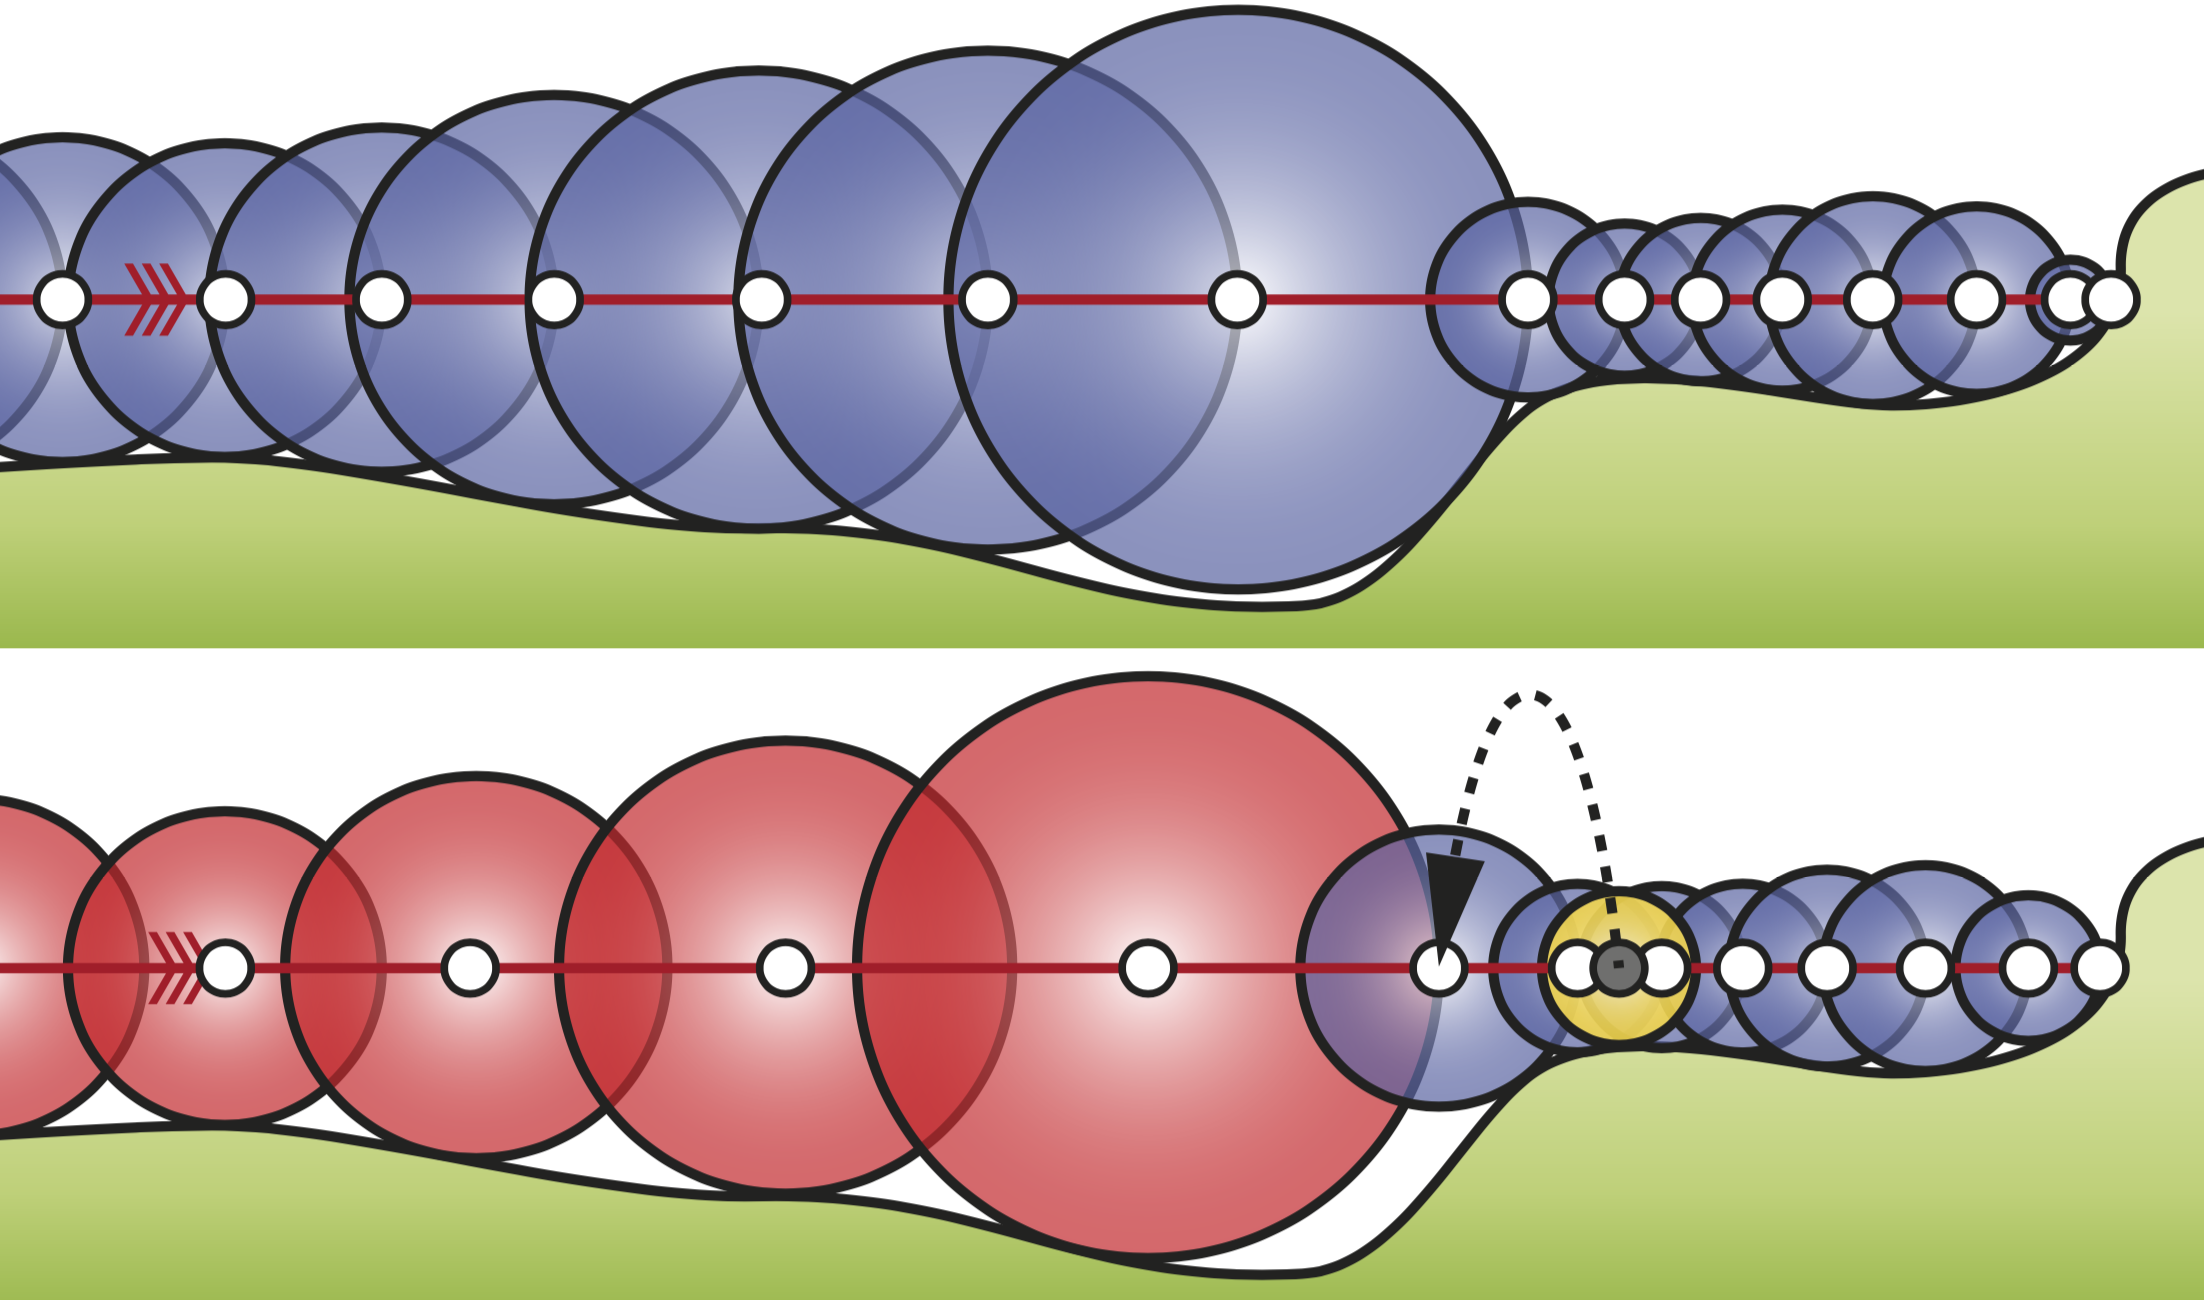
\includegraphics[width=0.65\textwidth]{figures/df/over-relaxation}
	\caption{使用(下图) 和不使用(上图)超松弛方法的 两种球体追踪的比较示意图,蓝色圆形为标准的球体追踪迭代,红色为使用 超松弛方法的迭代,其中 $\omega = 1.6$,蓝色的圆形表示 超松弛步进失败的位置,此时对其纠正回到标准的球 体追踪,如虚线箭头所示(图片来自\cite{a:Enhanced-Sphere-Tracing})}
	\label{f:df-over-relaxation}
\end{figure}

但是另一方面,由于球体追踪并不是一个线性方程组,所以当超松弛方法 失败时,它并没有一个纠正机制,所以超松弛可能导致步进的增量越过一些物 体,这就需要一种手动的机制来处理这种情况,即我们需要一种方法能够将步 进增量回退到一个合适的位置。

无论什么时候,只要原始球体追踪算法中两个相邻的采样位置及其距离值 形成的两个球体之间存在交集,那么光线线段在这两个球体形成的联合的区域 内就是绝对不会与表面相交的,即我们至少应该保证相邻两此步进的球体之间 存在交集。使用这个标准,我们可以很容易地判别处超松弛方法会失败的位置, 从而阻止继续使用超松弛方法,然后让这次步进过程回归到原始标准的球体追 踪中。即虽然我们没有了自动纠错机制,但是我们有一种方法能够在错误发生 之前及时阻止错误的发生。

具体地,如果 $|f(p_i−1)| + |f(p_i)|< \delta_{i−1}$,则超松弛方法可能会错失一个表 面的交点,在这种情况下,我们停止使用超松弛方法,而是回到标准的球体追 踪方法,其纠正后的开始位置为:

\begin{equation}
	p_{\rm fallback}=p_i+d\cdot \delta_{i-1}\cdot (1-\omega)
\end{equation}

在图\ref{f:df-over-relaxation}下图中,最后一次使用超松弛的正确位置为最右边的红色球体, 对其继续使用超松弛步进,则其下一个位置应该是黄色球体的位置,然后此时 黄色球体与红色球体并不存在交集,此时就有可能发生错误,当然这是一个保 守估计,很为很难有更精确的判断方法。所以在此种情况下,我们就放弃超松 弛步进,回滚到传统的球体追踪,即使用当前位置处的距离值作为步进增量,那么下一次正确的位置就位于红色球体的球面与光线的交点处,即虚线箭头指向 的球体位置。

\cite{a:Enhanced-Sphere-Tracing}同时还介绍了其它一些优化方法,这里不再一一介 绍,感兴趣的读者可以自行阅读。




\section{移位映射}
通过前面三节的内容,我们详细讨论了表面表述的基本概念,以及距离场 的表述和渲染方法,本章最后两节,我们来介绍两种距离场的应用。这两种应用 分别被用来解决不同的问题,其中本节将介绍使用距离场来实现移位映射,而下一节将讨论怎样使用距离场来计算可见性。

表面的细节按照尺寸可以划分为三种类型,微观结构,中观结构以及宏观结构。其中微观结构(microstructure)\myindex{微观结构}{microstructure}是一种非常小的细节,它对我们的肉眼 通常是不可见的,所以我们通常不会显式地表述它,而是使用一种统计模型来 表述它的光照散射特征,这种统计模型即是本书前面介绍的双向反射分布函数(bi-directional reflectance distribution function,BRDF)\myindex{双向反射分布函数}{bi-directional reflectance distribution function};而宏观结构(microstructure)\myindex{宏观结构}{microstructure}则是比较大的几何细节,这种细节通常使用如三角形网格来表述,这通过建模来实现,它表述的是物体表面的宏观特征。

而中观结构(mesostructure)\myindex{中观结构}{mesostructure}则是一种介于微观和宏观直接的表面几何细 节,如图\ref{f:df-meso-structure}所示,它们是一种几何细节,这意味着我们可以使用图形学的方法来控制它,然而却很难用网格和三角形模型来描述它,因为那样模型的顶点数量将会非常巨大,我们可以理解为就是一个三角形基元内部的几何细节。然而这些几何细节却非常重要,它们可以很明显地影响着阴影遮挡的计算。在计算机图形学中,我们通常使用移位映射技术来表述物体表面的中观结构。

\begin{figure}
\begin{fullwidth}
	\begin{subfigure}[t]{0.17\thewidth}
		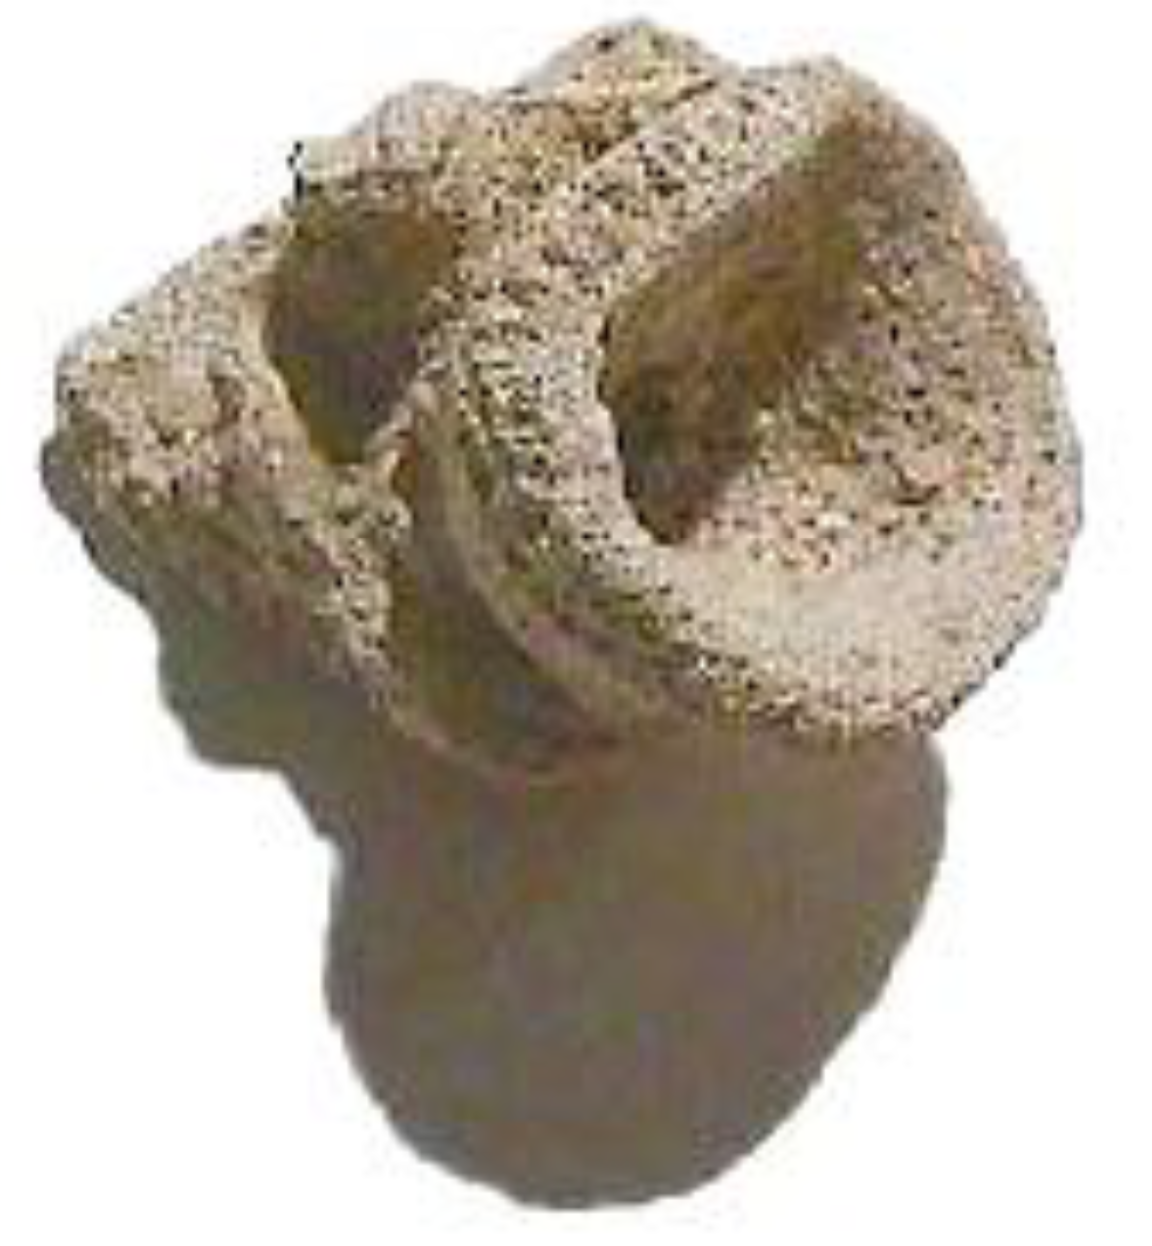
\includegraphics[width=\textwidth]{graphics/df/meso-structure-1}
		\caption{Sponge}
	\end{subfigure}
	\begin{subfigure}[t]{.285\thewidth}
		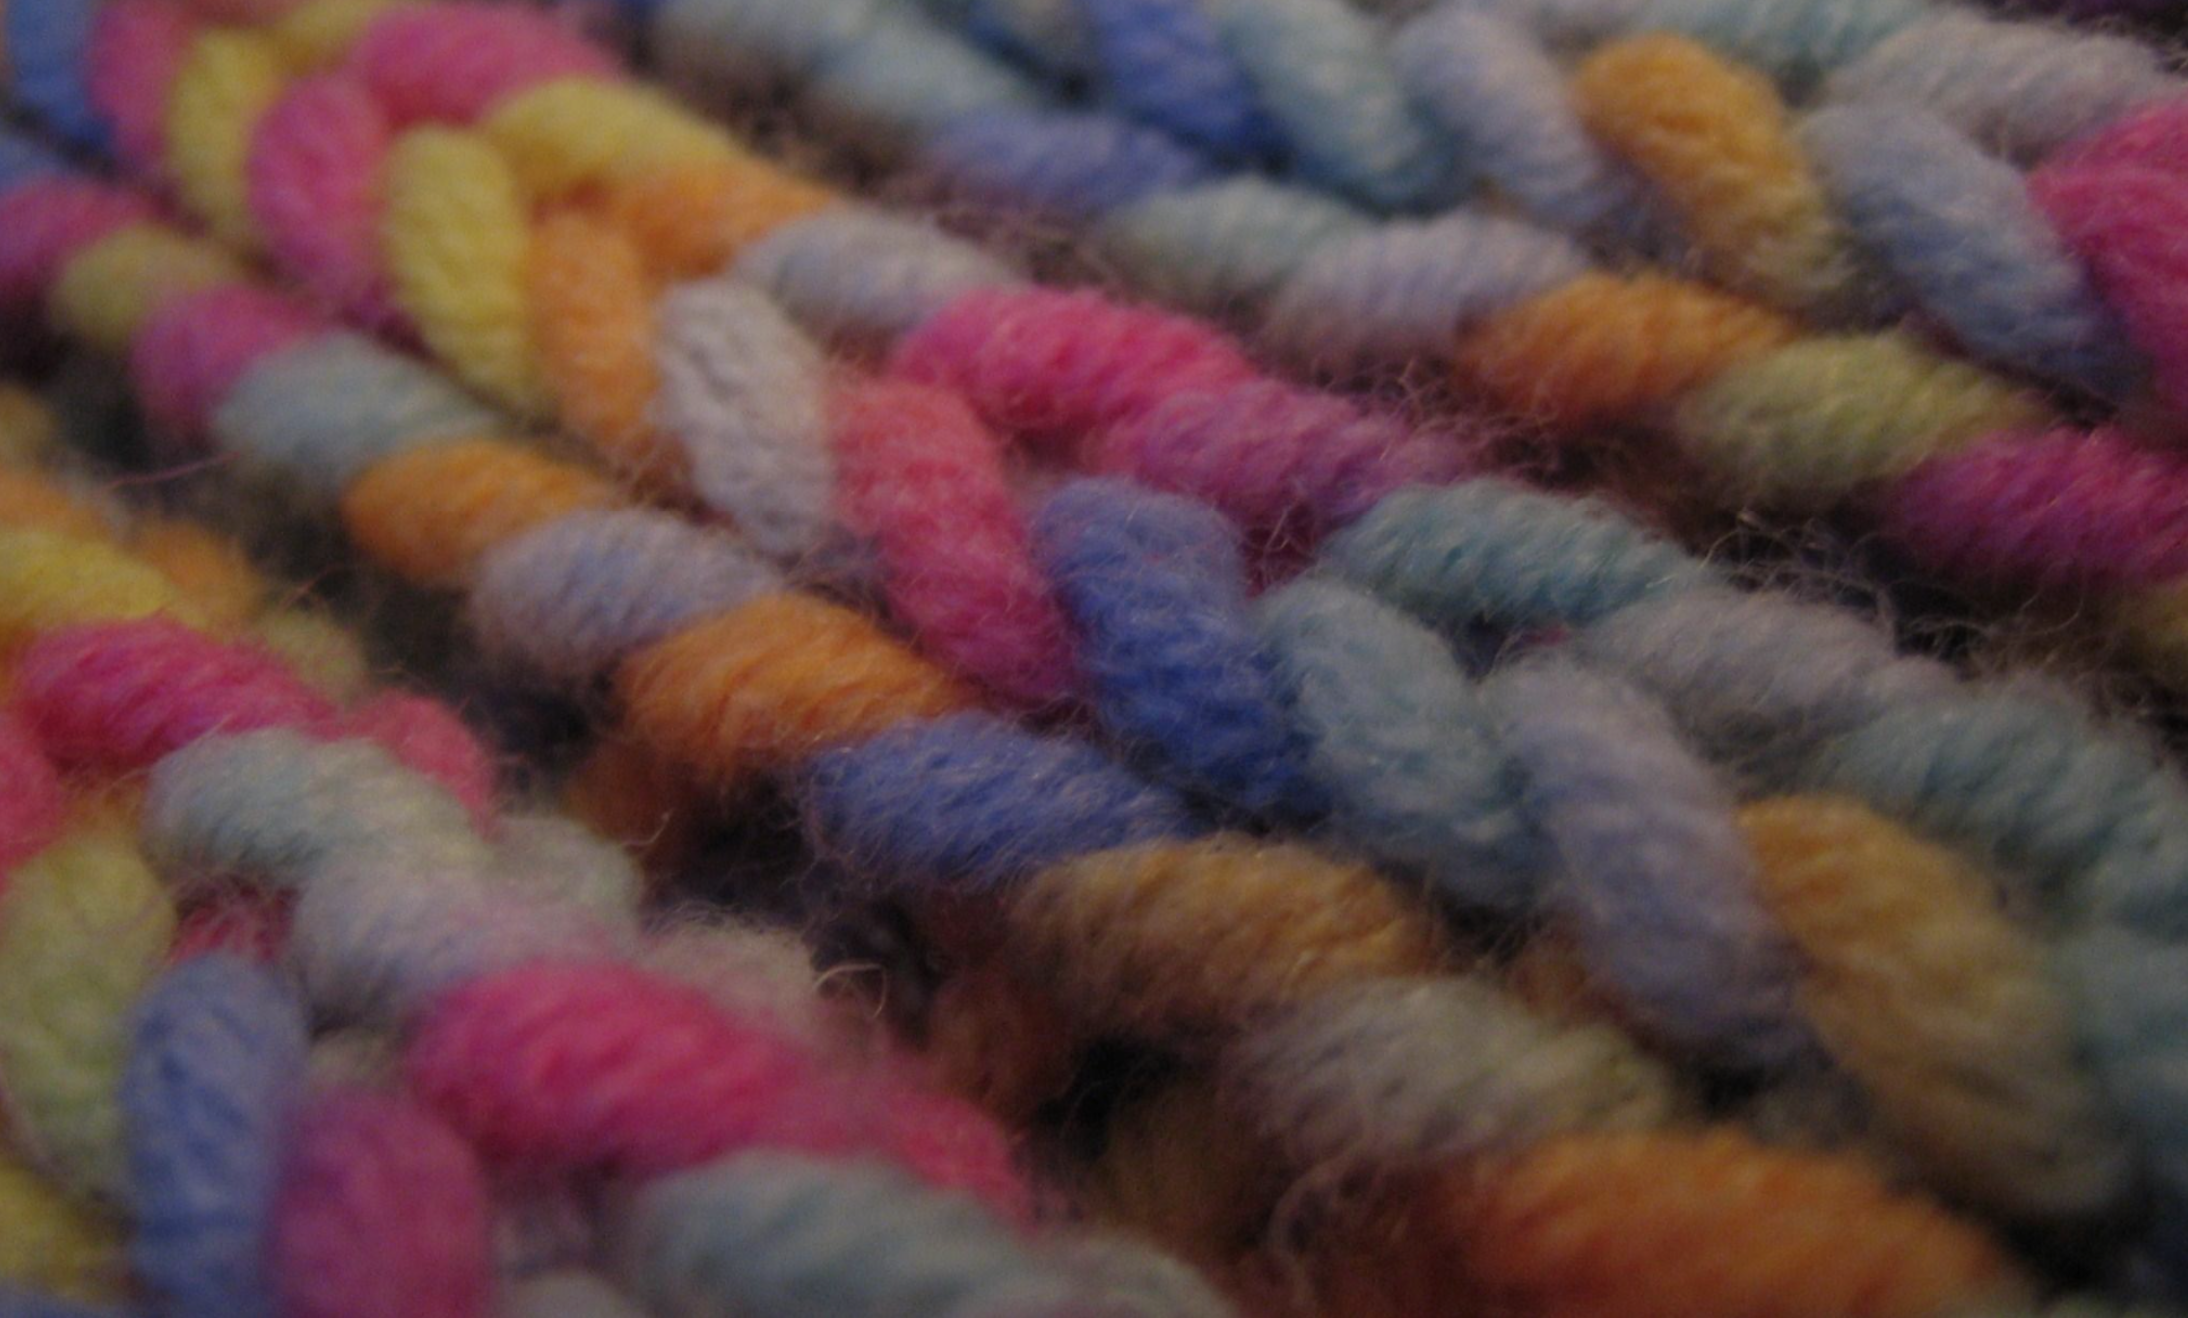
\includegraphics[width=\textwidth]{graphics/df/meso-structure-2}
		\caption{Cloth}
	\end{subfigure}
	\begin{subfigure}[t]{.23\thewidth}
		\includegraphics[width=\textwidth]{graphics/df/meso-structure-3}
		\caption{Tree}
	\end{subfigure}
	\begin{subfigure}[t]{.26\thewidth}
		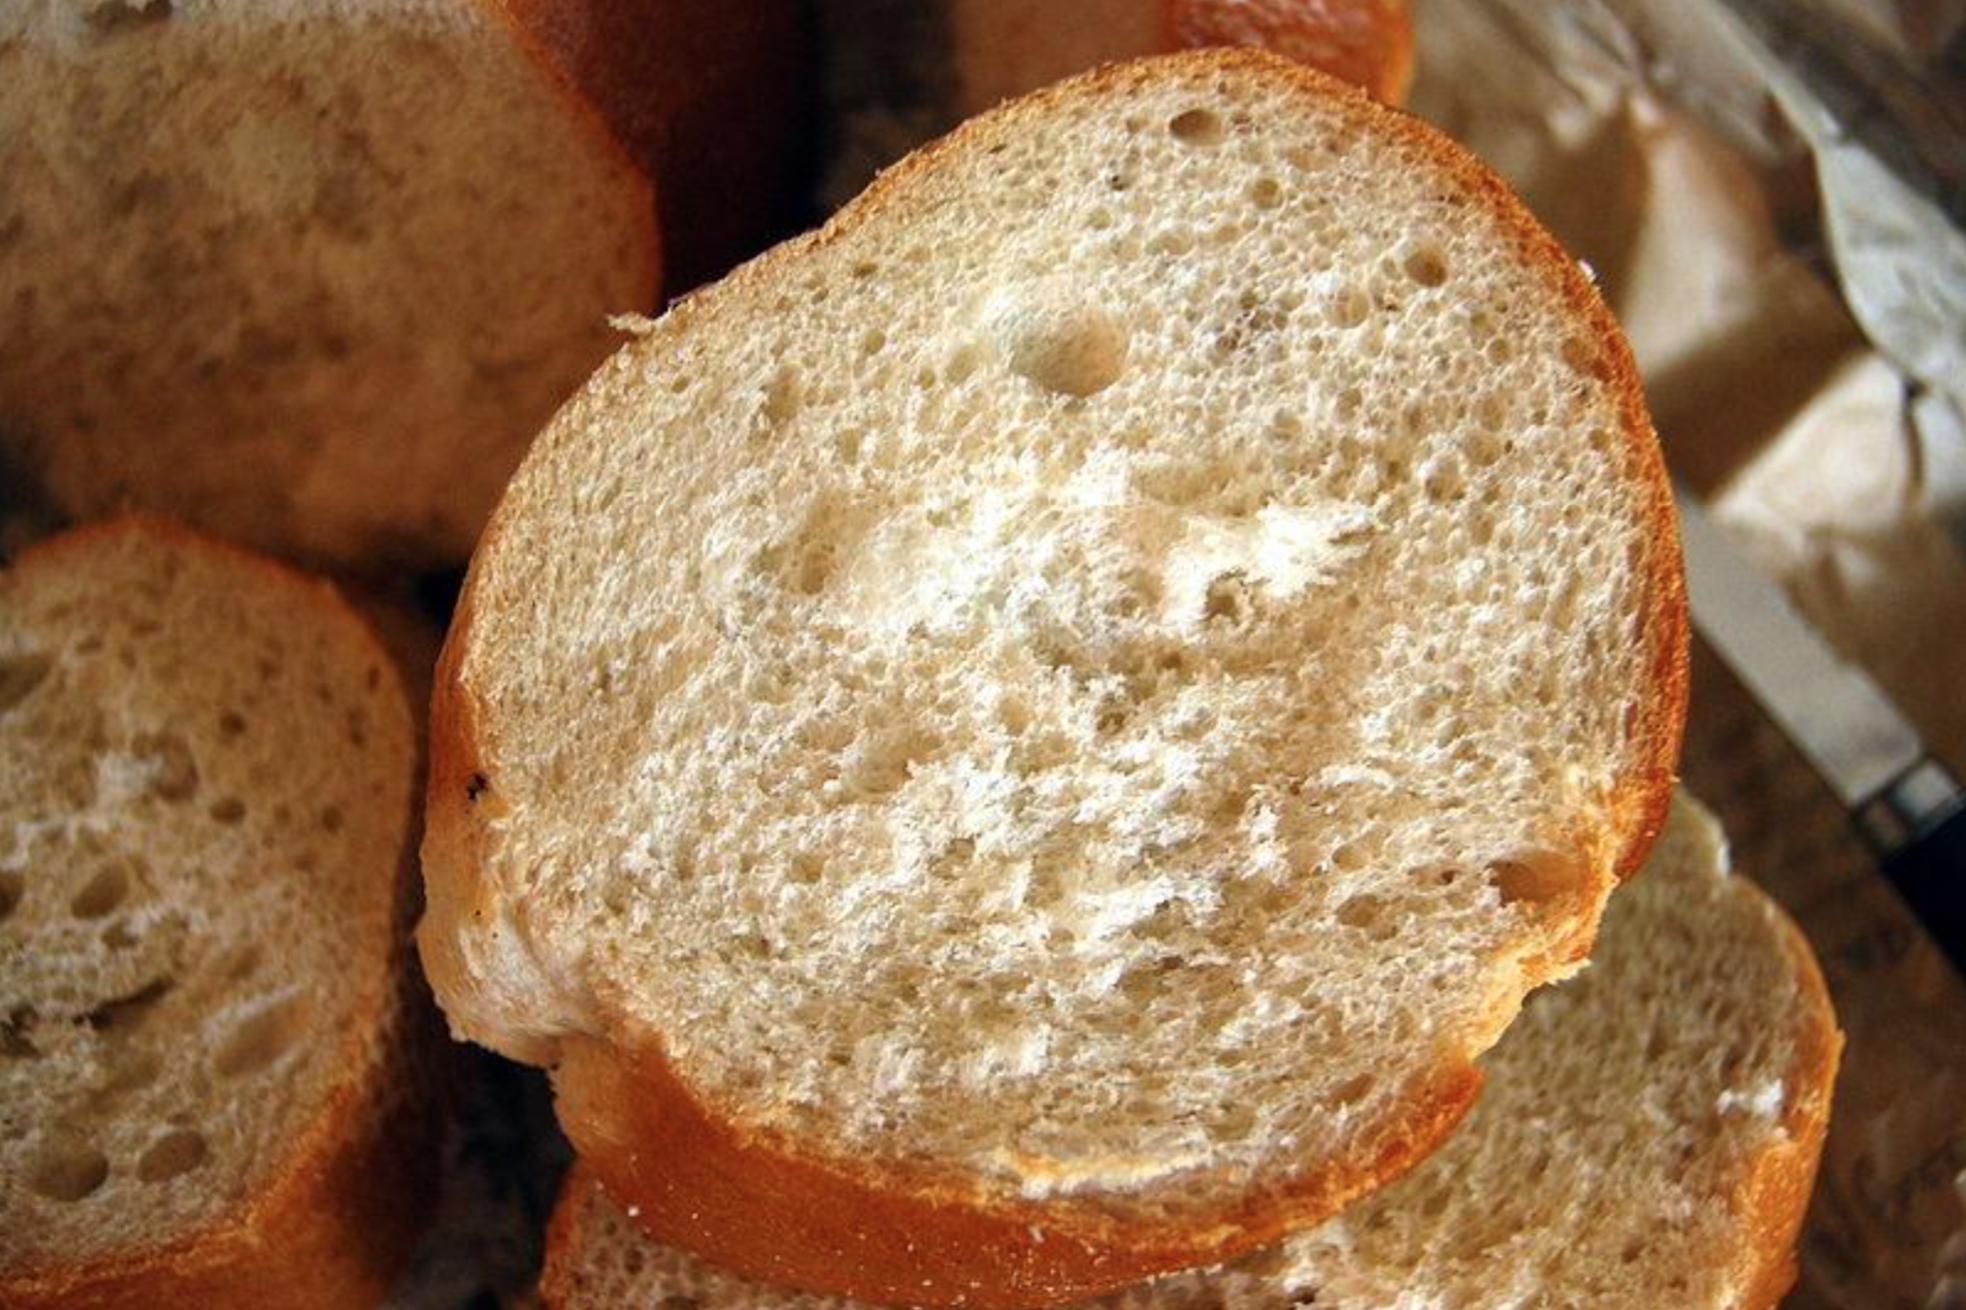
\includegraphics[width=\textwidth]{graphics/df/meso-structure-4}
		\caption{Bread}
	\end{subfigure}
	\caption{图中展示了一些常见的表面中观结构,这些结构通常是体积结构,不容易使用常用的平面贴图来表述,也很难实现交互式甚至实时的渲染需求}
	\label{f:df-meso-structure}
\end{fullwidth}
\end{figure}



\subsection{什么是移位映射}
为了给物体表面添加这种中观结构的细节,\cite{a:Shade-Trees}提出了移位映射(displacement mapping)\myindex{移位映射}{displacement mapping},与传统的凸凹映射(bump mapping)\myindex{凸凹映射}{bump mapping}\cite{a:SimulationofWrinkledSurfaces} [Blinn, 1978] 仅仅影响表面着色不同的是,移位映射会修改物体表面元素的位置,即虽然一个三角形内部的表面元素都是位于一个平面上的,但是移位映射修改了这些元素的位置,使它看起来形成了一种真正的中观几何结构。虽然\cite{a:DetailedShapeRepresentationwithParallaxMapping}提出的视差映射(parallax mapping)\myindex{视差映射}{parallax mapping}也可以实现纹理坐标的移位,这通过一个在正切空间的关于观察视角的函数和一个高度图来实现,但是这个过程并不包含对阴影遮挡的计算,而移位映射可以修改阴影,遮挡以及剪影。 

目前通常有两种关于移位映射的实现,其中一种迭代式地对一个基础表面执行细分(tessellate)\myindex{细分}{tessellate}操作,并将顶点朝表面法线的方向推挤,该操作一直持续 直到其产生的细分几何体的尺寸接近于一个像素的尺寸。这种方法依赖于硬件支持,例如DirectX 11 的曲面细分(tessellation)\myindex{曲面细分}{tessellation}就提供一种在曲面细分阶段 修改顶点的能力,该算法通常在顶点着色器中实现。\cite{a:AdaptiveTessellationofSubdivisionSurfaceswithDisplacementMapping} 演示了这 种方法,该方法的实质是:“对于几何体的每一个小区域,它将被映射图像上的哪一个像素?” 

另一种被讨论的比较多的方法是基于光线追踪的方法,这种方法并不依赖于几何细分,它通过在像素着色器中从观察方向对一个高度图或者 3D 体积纹 理执行光线追踪来计算与该光线相交的表面上的真实位置,这种方法也即是本 节将要讨论的方法。与基于细分的方法不同,像素着色器通常会比顶点着色器 更快,并且像素着色器被优化于更高效地读取纹理数据,此外,通过使用像素 着色器,这避免了产生大量的临时的顶点数据,这大大节省了内存占用。光线追踪算法的实质是:“对于图像上的一个像素及观察方向,它能看到几何体中的哪一部分?”

有很多基于光线追踪的方法被用于实现移位映射,本节我们主要聚焦于基 于使用距离场来表述移位数据的方法,我们会发现,这是一种非常高效且能产 生高质量图像细节的方法。



\subsection{浮雕映射}
我们要讨论的第一种移位映射方法将聚焦于简单的平面物体上,这种方法 其实并没有使用距离场表述,但是首先介绍这种简单的情形有利于我们了解基 于光线追踪的移位映射算法的基本结构及思路。

\cite{a:Real-TimeReliefMappingonArbitraryPolygonalSurfaces}基于在 GPU 上实现的一个高效的光线与高度图相 交算法,提出了一种称为浮雕映射(relief mapping)\myindex{浮雕映射}{relief mapping}的技术,这种技术实现一 个 2D 的高度图来实现光线追踪,当然在次年\cite{a:ReliefMappingofNo-Height-FieldSurfaceDetails}又实现了一个不需要高度图的改进算法,这里我们注重基本思路,所以以第一种为例进行介绍。

图\ref{f:df-relief-mapping-representation}展示了一个使用一个深度贴图和法线贴图表述的浮雕纹理,其中深度图被表述为一个 $RGB\alpha$ 纹理的 $\alpha$ 通道,其RGB通道则存储着法线值,这样一个32 位的纹理就足以表述一个浮雕纹理。

\begin{figure}
\sidecaption
{
	\begin{subfigure}[t]{0.31\textwidth}
		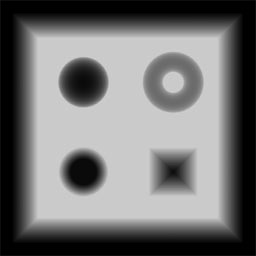
\includegraphics[width=\textwidth]{graphics/df/relief-mapping-representation1}
	\end{subfigure}
	\begin{subfigure}[t]{0.31\textwidth}
		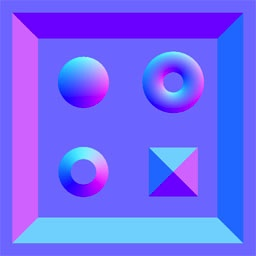
\includegraphics[width=\textwidth]{graphics/df/relief-mapping-representation2}
	\end{subfigure}
}
	\caption{一个浮雕纹理被表述问一个深度贴图(左)和一个法线贴图(右), 其中 法线值被映射到 $[0,1]$ 坐标 范围并且存储在一个 RGB 图表,深度值被归一化到 $[0,1]$,从上往下,甚至值从 0.0 变化到 1.0(图片来 自 \cite{a:Real-TimeReliefMappingonArbitraryPolygonalSurfaces})}
	\label{f:df-relief-mapping-representation}
\end{figure}

将浮雕数据映射到一个多边形表面的过程在概念上可以划分为以下步骤, 其中对于每一个待渲染计算的像素:

\begin{enumerate}
	\item 计算可视方向 VD,这是一个从观察点指向多边形表面上某个位置的一个 方向矢量,并将 VD 矢量变换到正切空间,这个过程的结果产生一条光线。
	\item 使用VD和A来计算B,其中A为像素使用的纹理坐标$(s,t)$,而B为光 线达到深度值为 1.0 处的纹理坐标 $(u, v)$,如图\ref{f:df-relief-mapping}中的 $textcircled{A}$ 和 $textcircled{B}$ 所示。
	\item 在光线 VD 方向上,以及 A 和 B 之间通过二分搜索方法查找光线与用高 度表述的表面的交点,如图\ref{f:df-relief-mapping}(a) 所示。
	\item 最后使用上一步得到的交点位置作为像素着色器实际使用的纹理坐标位置。
\end{enumerate}

上述的过程可以参见图\ref{f:df-relief-mapping}(a) 所示,实践中他们发现 8 次二分细分就足以产生非常令人满意的结果,这等效于将深度场的范围细分为 $2^{8} = 256$ 个相 等的空间间隔。该方法同时也利用了图形处理器的线性插值特性,由于深度值 被当做一个纹理,因此纹理的线性插值保证了高度图表面是连续的。

\begin{figure}
\begin{fullwidth}	
	\begin{subfigure}[t]{0.33\thewidth}
		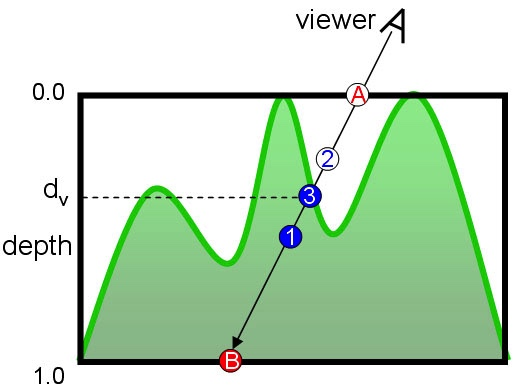
\includegraphics[width=\textwidth]{graphics/df/relief-mapping1}
		\caption{Binary search}
	\end{subfigure}
	\begin{subfigure}[t]{.33\thewidth}
		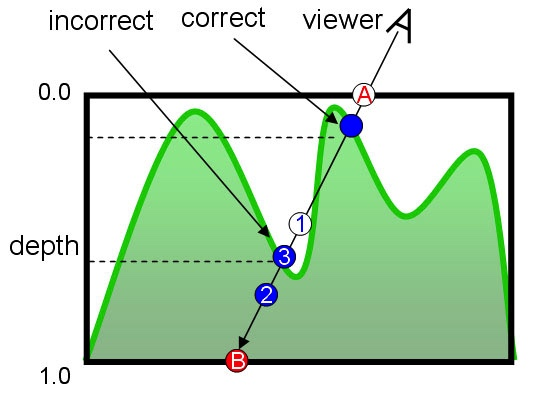
\includegraphics[width=\textwidth]{graphics/df/relief-mapping2}
		\caption{Incorrect}
	\end{subfigure}
	\begin{subfigure}[t]{.33\thewidth}
		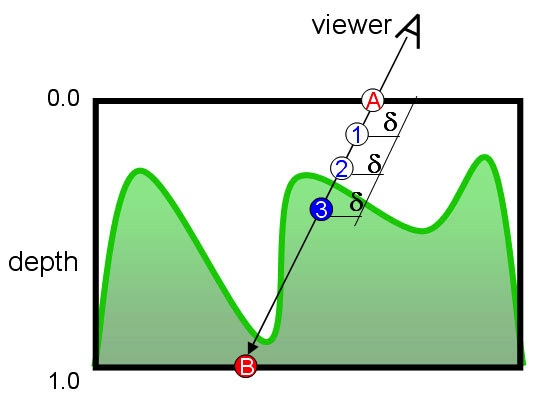
\includegraphics[width=\textwidth]{graphics/df/relief-mapping3}
		\caption{Linear search}
	\end{subfigure}
	\caption{浮雕映射的实际过程是首先使用线性搜索 (c) 找到光线在表面内的第一个交点,即 (c) 中的点$\textcircled{3}$,然后在点$\textcircled{2}$ 和$\textcircled{3}$ 时间使用二分搜索 (a) 查找表面上的第一个交点(图片来自\cite{a:Real-TimeReliefMappingonArbitraryPolygonalSurfaces})}
	\label{f:df-relief-mapping}
\end{fullwidth}
\end{figure}

如果观察光线同时穿过高度图表面上两个及以上的位置,则上面刚刚描述 的二分搜索过程可能导致不正确的结果,如图\ref{f:df-relief-mapping}(b) 所示。为了避免可能错 失第一个交点的结果,这里首先使用一个线性搜索并找到位于表面内的第一个点,如图\ref{f:df-relief-mapping}(c) 中的点 $\textcircled{3}$ ;一旦第一个位于高度图表面内部的点被找到,然 后再在该点和最后一个(该次线性搜索过程中)位于高度图表面外的点(即如 图\ref{f:df-relief-mapping}(c) 中的点 $\textcircled{2}$ )之间执行二分搜索,这个过程有点类似于前面介绍的光 线步进过程。

然而不幸的是,线性搜索要求使用一个固定的步进尺寸,这意味着为了捕 捉较小的表面细节,我们可能需要增加步进的次数,这就要求我们在精度和性 能之间做出一个权衡。

使用上述类似的过程,我们可以计算处阴影光线与高度场的交点。



\subsection{基于距离场的移位映射}
基于上述的浮雕映射技术,\cite{a:Per-PixelDisplacementMappingwithDistanceFunctions}提出了一种改进方法,该方法使用一个距离场来替代高度场,所以这允许使用球体追踪来自动地调整光线步 进的尺寸,这使得我们可以在靠近表面的位置使用更小的步进尺寸以捕获足够 精细的细节,而在那些远离表面或者较大的空白区域可以使用较大的步进尺寸,以加快步进的速度。

为了创建一个距离场纹理,该算法首先创建一个 3D 贴图,其中每个像素 存储着它到离其最近表面的一个移位矢量,然后基于这些位移矢量,执行一系 列的传输操作,将这些表面的位移矢量扩散到整个 3D 空间,这即是本章前面 介绍的距离变换。一旦所有 3D 空间中的位移被计算出来,该位移矢量的大小 就作为距离场中的距离值。

\begin{figure}
	\sidecaption
	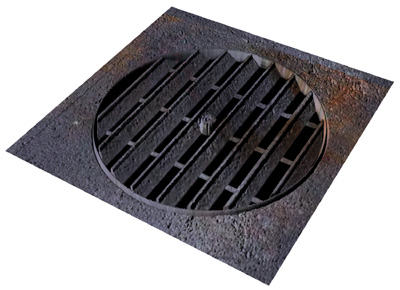
\includegraphics[width=0.5\textwidth]{figures/df/08_displacement_06}
	\caption{使用基于距离场的移位映射技术渲染的物 体,可以看到其保留了非常好的中观结构细节(图片来自 \cite{a:Per-PixelDisplacementMappingwithDistanceFunctions})}
	\label{f:df-08_displacement_06}
\end{figure}

最后我们便可以使用球体追踪来计算光线与使用距离场表述的表面的相 交,这种方法要比上一节介绍的使用线性和二分搜索组合算法的浮雕映射技术 要高效得多。

算法的其它部分基本上上浮雕映射技术相似,首先观察光线被变换到正切 空间,然后使用球体追踪来计算光线与表面的交点。

在他们的实验中,对于较复杂的表面其距离场纹理的分辨率最大到 $512\times 512\times 32$,实际上论文中所有的例子仅使用 $512\times 512\times 16$ 的分辨率,通常迭代 8 次对于较平滑的表面就能产生比较精确的结果,最大迭代次数则为 16,这比 浮雕映射中的步进次数要少得多。

尽管如此,基于距离场的体积表述为会占用相当大的内存,在接下来的内 容中我们将介绍一些改进方法。




\subsection{壳形映射}
到目前为止,我们介绍了一些基于光线追踪的移位映射技术的基本概念和思路,这些方法都主要聚焦于平面表面上,现在我们将把注意力转向一般的平 面。本节我们将会讨论两个方面的问题,怎样表述任意的表面,以及怎样处理 随之而来的问题,即纹理扭曲。

虽然大多数 2D 的纹理足够用来表述一些简单几何物体的表面,但是它们 却很难表述比较复杂的中观结构的几何表面细节,因此我们需要使用 3D 的体 积纹理来表述这些中观结构的细节,这就需要对表面进行 3D 的参数。

\cite{a:Shell-Maps}提出了称为壳形空间(shell space)\myindex{壳形空间}{shell space}的概念,壳形空间是一个定义于一个基础表面(base surface)\myindex{基础表面}{base surface}$S$ 和其对应的一个偏移表面(offset surface)\myindex{偏移表面}{offset surface}$S_o$ 之间的有界区间,一个壳形贴图(shell map)\myindex{壳形贴图}{shell map}是指壳形空间 与纹理空间之间的一个双向映射函数,如图\ref{f:df-shell-maps-1}所示。通过使用壳形空间和壳形贴图,我们可以使用一个很薄的 3D 体积纹理来表述一个几何表面的中观结 构细节,这个概念就类似于使用一个 2D 的纹理来表述几何表面的法线分布。

\begin{figure}
	\sidecaption
	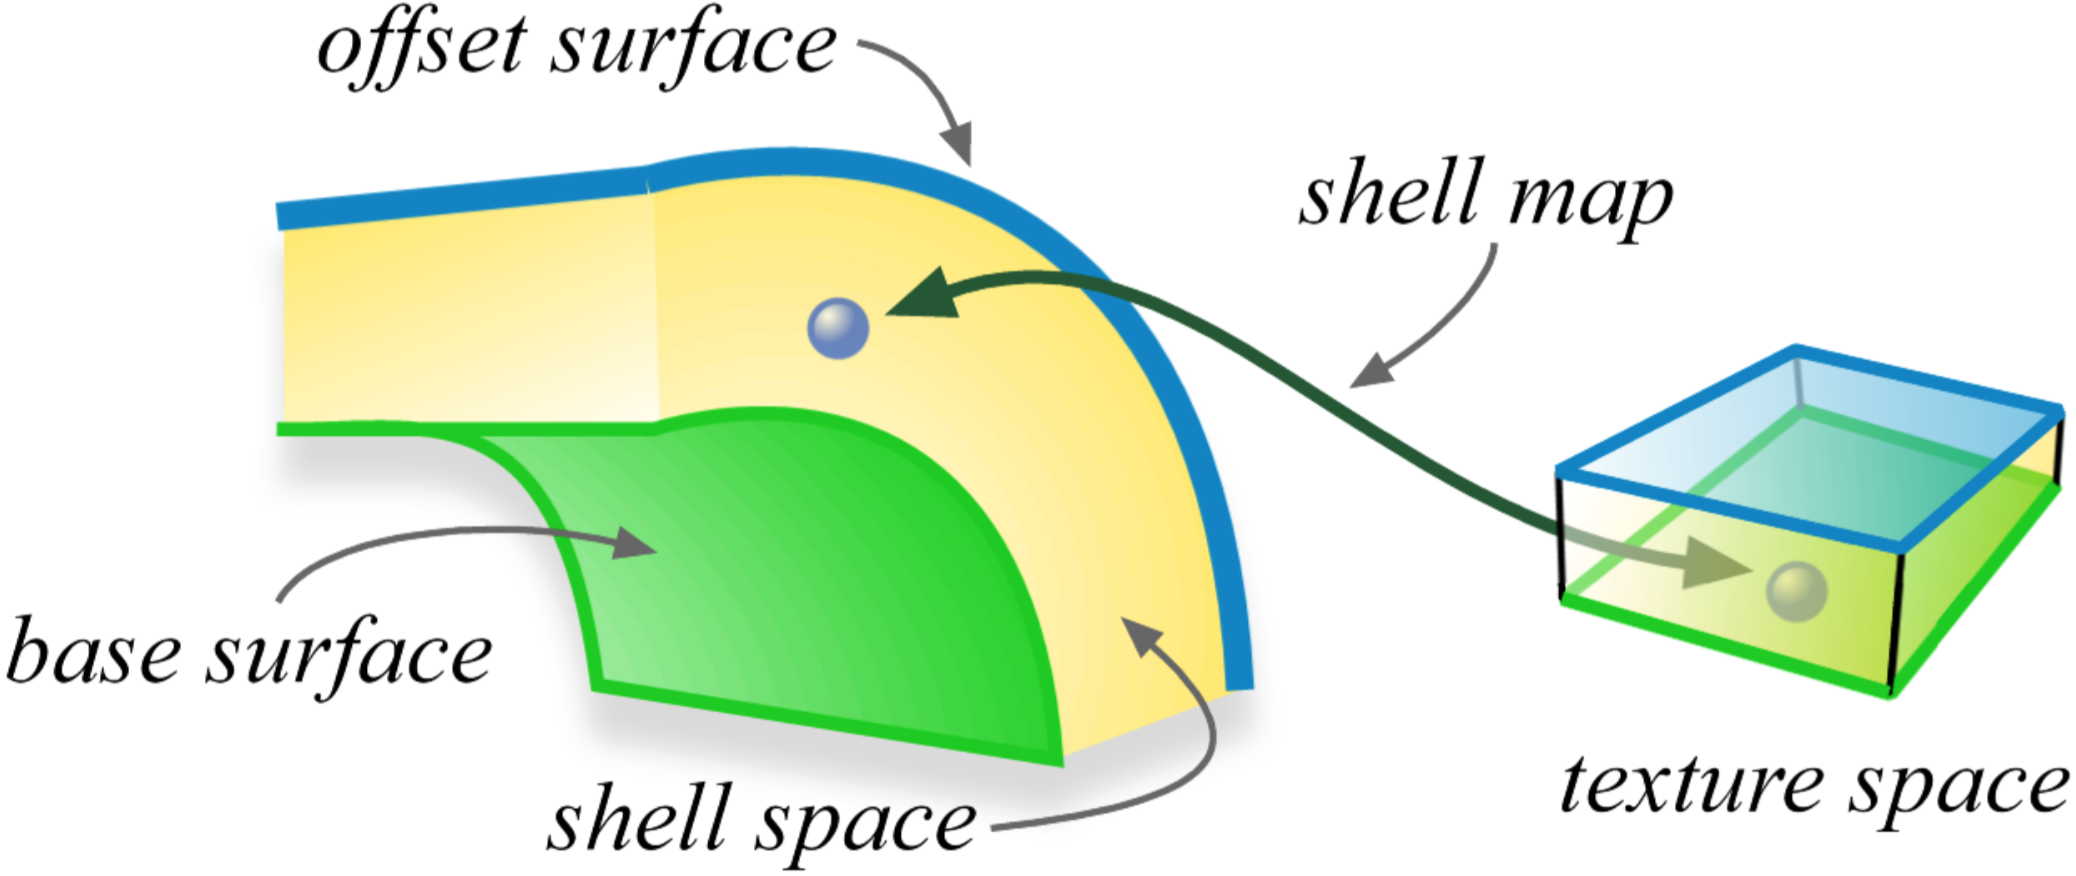
\includegraphics[width=0.65\textwidth]{figures/df/shell-maps-1}
	\caption{壳形空间是介于一个基本表面和一个其对应的偏移表面之间的空间,一个壳形贴图表示一个3D纹理到壳形空间的一个一对一的映射函数(图 片来自 \cite{a:Shell-Maps})}
	\label{f:df-shell-maps-1}
\end{figure}

上一节的内容仅仅将距离映射作用于一个平面上,通过使用壳形贴图,我 们可以将这种方法运用到一般表面上去。通过将 $S$ 中的每一个三角形沿其法线 方向挤压就会形成壳形空间中的一个棱柱,每个壳形空间中的棱柱在 3D 纹 理空间有一个对应的棱柱,这通过使用壳形空间中的顶点的坐标来生成,如图\ref{f:df-shell-maps-2}所示。

\begin{figure}
	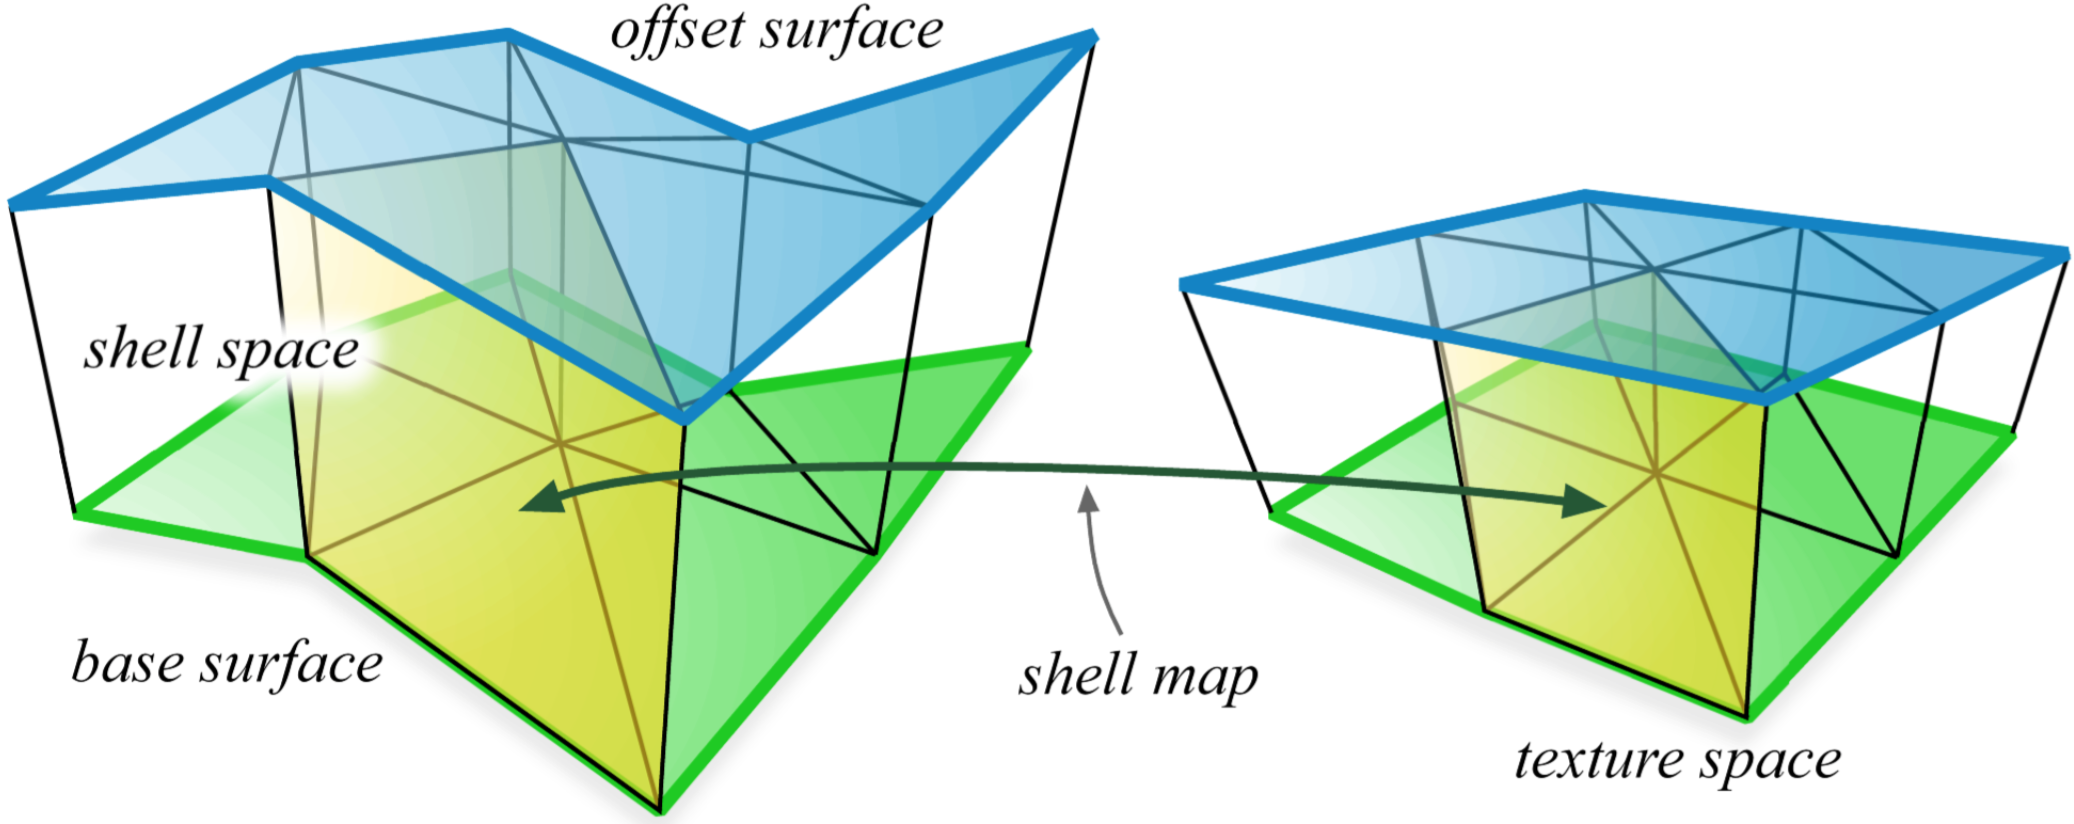
\includegraphics[width=\textwidth]{figures/df/shell-maps-2}
	\caption{壳形空间中每个三角形形成的棱柱,在 3D 纹理空间中都有一个对应的棱柱(图片来自 \cite{a:Shell-Maps})}
	\label{f:df-shell-maps-2}
\end{figure}

对于偏移表面的生成,他们采用了\cite{a:SimplificationEnvelopes}的算法,首先 $S_o$ 通过复制 $S$ 得到一个初始值,这建立起来在两个网格(即基础表面和偏移表面) 之间三角形和顶点的对应关系,$S_o$ 中的顶点被赋予了和 $S$ 中对应顶点一样的 纹理坐标。每个 $S$ 中的顶点 $\mathbf{v}$ 被赋予一个“方向”矢量 $\vec{d}$,它表示的是共享该顶 点的所有三角形的法线的一个线性组合。最后再将 $S_o$ 中对应于 $S$ 中顶点 $\mathbf{v}$ 的 顶点 $\mathbf{v}_o$ 沿该方向矢量向外迭代式地移动,读者可以参考原始论文获得相关的详细细节。

为了保持比较好的表面细节,整个表面的偏移距离最好保持一个常数,当 然我们也可以构建出一个任意的偏移表面,但是一般它需要满足以下两个属性, 否则就会导致扭曲:

\begin{itemize}
	\item $S$ 和 $S_o$ 必须相同数量的三角形,以及这些三角形之间相同的连通性,每个 三角形$\tau\in S$ 必须唯一地关联着另一个三角形 $\tau_o \in S_o$,每个顶点 $\mathbf{v}\in S$ 必 须唯一地关联着另一个顶点 $\mathbf{v}_o\in S_o$。
	\item $S_o$ 内的三角形之间必须不能相互相交,它们也不能与 $S$ 相交。
\end{itemize}


纹理空间的棱柱用于是正三角形棱柱,如图\ref{f:df-shell-maps-3}右边小图所示,但是壳形空间 内的棱柱却有可能不是凸多边形,所以为了创建一个健壮的映射,这里将棱柱 划分为三个四面体,这通过对每个四边形执行三角化来实现,如图\ref{f:df-shell-maps-3}所示。 通过对棱柱 $P$ 和 $P_t$ 使用相同的划分方式(这里主要是指对每个四边形面使用 相同方向的三角化),我们可以建立起纹理空间和壳形空间内每个四面体的联系,即每个壳形空间里的四面体 $T$ 在纹理空间关联着唯一一个四面体 $T_t$。

\begin{figure}
	\sidecaption
	\includegraphics[width=0.65\textwidth]{figures/df/shell-maps-3}
	\caption{棱柱被划分为三个四面体,根据每个四边形三角化的方向不同,棱柱有6种不同的划分方法,可以分别使用标记 FRR, RFR, RRF, RFF, FRF和 FFR 来表述不同的划分方法(图片来自 \cite{a:Shell-Maps})}
	\label{f:df-shell-maps-3}
\end{figure}

给定壳形空间里的一个四面体 $T$,以及纹理空间中对应的四面体 $T_t$,任意 一个 $T$ 中的点 $p$ 都可以被关联着 $T_t$ 中的唯一一个点 $p_t$,这通过贝叶斯坐标\footnote{如果$\mathbf{v}_1,\mathbf{v}_2,\mathbf{v}_3$ 和$\mathbf{v}_4$ 是一个四面体$T$ 的顶点,$p$是$T$ 中的一个点,则$T$ 中$p$的贝 叶斯坐标 $(\alpha_1, \alpha_2, \alpha_3, \alpha_4)$ 被定义为使得满足 $p = \alpha_1\mathbf{v}_1 + \alpha_2\mathbf{v}_2 + \alpha_3\mathbf{v}_3 + \alpha_4\mathbf{v}_4$,其中 $\alpha_1 +\alpha_2 +\alpha_3 +\alpha_4 =1$。}来 实现。这即是说,如果 $B(T,p)$ 定义为 $T$ 中 $p$ 的贝叶斯坐标,以及 $\phi(T,\alpha)$ 定 义为 $T$ 中贝叶斯坐标为 $\alpha$ 的点,则:

\begin{equation}
\begin{aligned}
	\mathbf{P}_t=&\phi(T_t,B(T,\mathbf{p})) \text{,~~和}\\
	\mathbf{p}=&\phi(T,B(T_t,\mathbf{p}_t))
\end{aligned}
\end{equation}

\noindent 建立起了壳形空间和纹理空间之间的双向映射。

一个程序化的或者几何纹理可以被使用光线追踪进行渲染,这只需要将世 界空间中的光线变换到纹理空间,然后在 3D 纹理中执行光线步进即可,然而 这种方法直接用在壳形映射中则会产生扭曲,如图\ref{f:df-shell-maps-5}所示,因为壳形空间中 的一个直线在纹理空间中可能是一条分片的曲线。

\begin{figure}
	\includegraphics[width=\textwidth]{figures/df/shell-maps-5}
	\caption{光线与壳形空间中的四面体相交(左),光线在壳形空间中步进,但是每个点被变换 到纹理空间以执行密度计算,这种方法有效地在纹理空间中对一个曲线进行追踪(右)(图片来自 \cite{a:Shell-Maps})}
	\label{f:df-shell-maps-5}
\end{figure}

为了解决这个问题,我们应该在壳形空间中执行光线步进,但是由于这些 距离值记录在纹理中,所以每一次步进之后需要将其位置变换到纹理空间去执 行密度计算以及光线和表面的相交计算。

在渲染时,首先还是对网格几何体进行光栅化,然后在每个像素着色器中 进行计算。对于每一个像素,我们将其所在的三角形向外挤压生成一个虚拟的 棱柱体,如图\ref{f:df-shell-maps-5}图所示,这里的观察光线为从摄像机到该像素的光线,我 们首先检查该光线在该棱柱体上端的第一个交点,然后从该位置开始在该三角 形对应的棱柱体内进行光线步进,其中每一步都需要将其坐标变换到纹理空间 去查询相关的距离值。最后如果在该棱柱体内找到一个表面上的交点,则该交 点的位置作为最终的着色位置,否则该光线会穿过该棱柱体,即说明该三角形 对当前的观察方向是完全不可见的,因此该像素被丢弃。

当然还有一些更聪明的方法,它们不需要在壳形空间执行光线步进,而是 直接存储一个与视角有关的高维纹理函数,有了方向信息,则就可以直接在纹理 空间执行查询即可。当然这种方法是使用存储空间换取了运行时的计算时间\footnote{但是这些方法也有缺点,因为这些方向信息是针对单个网格配置的预计算,所以一旦物体 的宏观几何结构发生了形变,则这些方法就容易发生失真。},在后面两节中我们将会讨论这样的方法。



\subsection{一般化的移位贴图}
\cite{a:GeneralizedDisplacementMaps} 基于一种称为一般化移位贴图(generalized displacement map,GDM)\myindex{一般化移位贴图}{generalized displacement map}的概念,提出了一种一般化的中观结构渲染技术,GDM 是 指在一个体积纹理内,其任意一点在一个指定方向上到最近的中观结构表面的 位置,简单理解就是对距离场中的每个体素加了一个方向信息,使之能获取每 单个(而不是所有)方向上的最近表面位置,因此这对距离场增加了一个新的 维度,需要占用更多的存储空间,但好处是,我们能够直接根据观察方向从纹 理中查到交点位置,这就避免了如上面的壳形映射方法在物体空间使用光线步 进来寻找交点。此外,GDM 也是同时考虑物体空间和纹理空间来进行交点,因 此能够降低纹理的扭曲。

该方法首先将带有中观结构的几何物体作为输入数据,并计算该物体的 GDM 数据(带方向信息的距离场),当 GDM 纹理被映射到这个物体的表 面之后,直接在像素着色器中对每个像素执行渲染,并直接从该 GDM 纹理中 查询与中观结构几何体的交点位置。

\begin{figure}
	\begin{subfigure}[b]{0.49\textwidth}
		\includegraphics[width=\textwidth]{figures/df/GDM-model-1}
		\caption{}
	\end{subfigure}
	\begin{subfigure}[b]{0.51\textwidth}
		\includegraphics[width=\textwidth]{figures/df/GDM-model-2}
		\caption{}
	\end{subfigure}
	\caption{GDM 模型:(a)GDM 定义为一个点 $P$ 在方向 $V$ 上距离固体表面最近的距离,(b) 展示了三种 GDM 的情况,从上至下:$P$ 位于体积外面并在 $V$ 方向与表面有一个交点,$P$ 在 体积外面但是在方向 $V$ 上与表面没有交点,$P$ 位于体积内,其 GDM 的值始终为 0(图片\cite{a:GeneralizedDisplacementMaps})}
	\label{f:df-GDM-model}
\end{figure}

如图\ref{f:df-GDM-model}所示,对于 GDM 纹理内的每一个位置 $p = (x, y, z)$,其采样方 向 $\vec{V} = (\theta,\phi)$ 被使用球面角度表述,其中的极角取值范围为 $\theta\in  [0,\pi]$,因此 GDM 是一个 5D 的函数,它记录了每个点沿观察方向上到最近的中观结构表 面位置的距离,即:

\begin{equation}
	d_{\rm GDM}(x,y,z,\theta,\phi)=\begin{cases}
		d & \text{如果光线与中观结构相交}\\
		d_{\max} & \text{如果光线方向上没有交点存在}\\
		0 & p\text{点位于体积内}
	\end{cases}
\end{equation}

其三种不同函数值的情况如图\ref{f:df-GDM-model}(b) 所示。

GDM 函数可以被映射到一个任意表面上,它就像一个传统的体积纹理 $V(x,y,z)$,只不过其中的每个纹素包含一个 2D 的函数 $(\theta,\phi)$ 用于存储方向 信息。将一个体积纹理映射到一个三角形网格上,其实就是会将该三角形网格 沿其法线方向向外推挤形成一个棱柱体积,如图\ref{f:df-GDM-space}(a) 所示。因此,对于在 物体空间中每个棱柱体(即对应于表面上的一个三角形面)对应的中观结构几 何,其在纹理空间中有一块唯一对应的(棱柱体)体积,如图\ref{f:df-GDM-space}(b) 所示。

\begin{figure}
	\begin{subfigure}[b]{0.49\textwidth}
		\includegraphics[width=\textwidth]{figures/df/GDM-object-space}
		\caption{物体空间}
	\end{subfigure}
	\begin{subfigure}[b]{0.51\textwidth}
		\includegraphics[width=\textwidth]{figures/df/GDM-texture-space}
		\caption{纹理空间}
	\end{subfigure}
	\caption{在物体空间,每个三角形面向外推挤形成一个立体的棱柱体体积 (a),每个物体空间的棱柱体体积都对应着纹理空间一个棱柱体体积 (b)(图片\cite{a:GeneralizedDisplacementMaps})}
	\label{f:df-GDM-space}
\end{figure}

与传统的体积纹理的渲染不同,GDM 渲染算法并不会在中观几何体中 执行光线追踪,它仅仅每次针对一个棱柱体内的一个线段执行快速处理,如 图\ref{f:df-GDM-space-ray}所示。前面已经说明,在物体空间中的一条光线,其方向在纹理空间 中会发生变化,如图\ref{f:df-GDM-space-ray}上面小图所示,因此为了避免扭曲,我们应该在物体空间 执行光线的穿行,但是这里并不需要像壳形映射算法那样在物体空间执行光线 步进,因为在纹理空间中已经能够直接获取任意一个点在任意一个方向上的最 近表面交点,所以这里使用一种巧妙的方式,使其光线在物体空间穿行,但是 其采样计算完全是在纹理空间。

\begin{figure}
\sidecaption
{
	\begin{subfigure}[b]{0.315\textwidth}
		\includegraphics[width=\textwidth]{figures/df/GDM-object-space-ray}
		\caption{物体空间}
	\end{subfigure}
	\begin{subfigure}[b]{0.315\textwidth}
		\includegraphics[width=\textwidth]{figures/df/GDM-texture-space-ray}
		\caption{纹理空间}
	\end{subfigure}
}
	\caption{路径在物体空间 和纹理空间的映射,GDM 算法正是利用这种线段之间 的映射来在纹理空间提供方 向信息,从而可以直接在纹 理空间进行采样,同时保证 了光线方向的正确性,因为 光线还是沿物体空间的方向 在穿行的(图片\cite{a:GeneralizedDisplacementMaps})}
	\label{f:df-GDM-space-ray}
\end{figure}

GDM 渲染的算法如下,其中这里计算的是以一个棱柱为单位:

\begin{lstlisting}[language=C++, mathescape=true]
PixelShading ($P_{\rm in}$, $T_{\rm in}$ ) 
	计算线段在棱柱体内的出射点($P_{\rm out}$, $T_{\rm out}$ ) 
	计算纹理空间内线段的长度 $d_t = |T_{\rm out} − T_{\rm in}$ | 
	计算纹理空间的观察方向 $V_t$
	查询GDM获得$p$点距离值 $d_{\rm GDM} (T_{\rm in}, V_t)$
	if ( $d_{\rm GDM} < d_t$ )
		计算相交点的纹理坐标 T
		着色计算
	else
		无相交点
\end{lstlisting}

GDM 的渲染流程和壳形映射算法的基础结构是类似的,首先对表面执行 光栅化,然后像素着色器得到表面上每个像素的位置,然后像素着色器首先根 据该像素的位置从摄像机发出一条观察方向,并根据该像素所在的三角形构建 一个虚拟的物体空间内的棱柱体,然后计算出观察方向与该棱柱体的入射点, 即上面算法中的 $P_{\rm in}$,同时得到其对应纹理空间中的坐标 $T_{\rm in}$,这两个参数形成 上述算法的输入参数。

GDM 算法的核心是在物体空间得到一个虚拟的线段,然后将该线段变换 到纹理空间,这通过计算两个空间内的入射点 $P_{\rm out}$ 和 $T_{\rm out}$ 来实现,其具体的过 程如下:由于光线必须在物体空间沿直线穿行,所以我们很容易在物体空间的 棱柱体中计算出出射点 $P_{\rm out}$,然后我们将该出射点变换到纹理空间得到 $T_{\rm out}$, 这就得到光线在纹理空间的穿行直线段 $T_{\rm in}T_{\rm out}$,然后就可以直接在纹理空间 从该直线段计算出交点位置,如图\ref{f:df-GDM-space-ray}所示。

既然找到了光线在纹理空间的穿行路径,这也就间接得到了光线在纹理空 间的方向,因此我们有了光线在纹理空间的起点位置 $T_{\rm in}$,以及该光线在纹理 空间的方向 $T_{\rm in}T_{\rm out}$,因此根据 GDM 的定义,我们就可以直接得到距离 $T_{\rm in}$ 点 最近的交点。我们可以看到这里完全避免了通过光线步进来求交点的过程,其 效率大大提高。




\subsection{有向的距离贴图}
基本上,基于 GPU 的光线-物体相交算法有两种策略,其中一种尝试将焦 点包含在两个点之间,然后在这段间隔内搜索求解,例如前面讨论的浮雕映射 算法就是这种类型。这种包围交点的过程依赖于不太健壮且低效的线性步进, 这会带来一些失真。

第二种策略基于空间跳跃(space skipping)\myindex{空间跳跃}{space skipping},它使用一些预计算的数据结 构来存储一个安全区域,使得在这个安全区域内不存在任何表面。然后交点的 搜索过程就可以在光线步进的过程中直接跳过这些安全区域,例如前面介绍的 距离贴图就是这种策略。这种技术的缺点是在靠近表面的区域其收敛速度很慢,并且需要占用很高的内存来存储 3D 空间数据,过低分辨率的 3D 数据则会导 致走样的发生。

为了应对这些缺点,\cite{a:directional-distance-maps}提出了有向距离贴图(directional distance map)\myindex{有向距离贴图}{directional distance map}的技术,相对于前面介绍的距离贴图和一般化的移位 贴图,这种技术有三个方面的重要贡献:

\begin{enumerate}
	\item 与方向有关的球体追踪能够实现更快速的收敛。
	\item 基于二次曲面的近似和相交计算能够提升渲染质量。 
	\item 无损的距离贴图压缩能够减少内存占用。
\end{enumerate}

受 GDM 算法的启发,该算法使用一个有向距离贴图来加速相交计算的收 敛速度,但是与 GDM 直接对体积纹理进行采样不同的是,这里仍然使用球体 追踪,其原因是 GDM 依赖于线性插值,其结果在放大后会有比较大的失真。

跟 GDM 的数据结构有点类似,一个有向距离贴图(directional distance map,DDM)\myindex{有向距离贴图}{directional distance map}中的每个体素 $V$ 存储的是一个有向的圆锥体范围内(而不是单个方向)距离该体素最近的中观结构表面距离。因此,覆盖整个表面的球面角度 $(\theta, \phi)$ 被划分为多个空间间隔,每个间隔形成一个有向的圆锥体,其中 $\theta$ 在水平方向由 0 到 $360^{\circ}$ 变化,而 $\phi$ 在垂直方向由 $−90^{\circ}$ 到 $+90^{\circ}$ 变化。如图\ref{f:df-ddm-comparision}(b)所示,在 $p_0$ 点以下的 $180^{\circ}$ 范围被划分为4个有向的圆锥体,当然这是在一个2D面上观察。

\begin{figure}
	\begin{subfigure}[b]{0.5\textwidth}
		\includegraphics[width=\textwidth]{figures/df/ddm-comparision-1}
		\caption{距离贴图}
	\end{subfigure}
	\begin{subfigure}[b]{0.5\textwidth}
		\includegraphics[width=\textwidth]{figures/df/ddm-comparision-2}
		\caption{DDM}
	\end{subfigure}
	\caption{基于距离贴图 (a) 和有向距离贴图的球体追踪的比较,注意后者在靠近中观结构的表面附近,以及整个空白空间都有更快的收敛速度(图片\cite{a:directional-distance-maps})}
	\label{f:df-ddm-comparision}
\end{figure}

由于每个距离值是对应于一个空间而不是一个特定方向,因此其光线与表 面的相交计算仍然需要使用球体追踪,而不是能够(像GDM算法一样)直接 查询到相交结果。但是通过方向的划分,这能够大大加速球体追踪的收敛速度, 例如在图\ref{f:df-ddm-comparision}中,如果没有方向划分,则距离 $p_0$ 点的最近表面点为右边第一个封顶,所以第一次步进距离就很小,如左图所示。但是划分成多个圆锥体之 后,左上的第一个圆锥体体积内的最近距离就要远得多,所以一次步进就能前进很远的距离,这就大大节省了步进的迭代次数,也即是减少了像素着色器中对距离场纹理的查询次数。

对于每一个体素,其对每个有向圆锥体分别计算一个距离值,对于中观结 构 $M$,纹理空间中的体素 $V$ ,以及有向圆锥体间隔 $[\theta_1, \theta_2] \times [\phi_1, \phi_2]$,DDM 的 数据结构可以表述为:

\begin{equation}
\begin{split}
	DDM(V,[\theta_{1},\theta_{2}]\times [\phi_{1},\phi_{2}])=min\{dist(\mathbf{m},\mathbf{v})\textrm{ }\forall\mathbf{m} & \in\mathbf{M},\\
	\textrm{ any } \mathbf{v} & \in\mathbf{V} \textrm{ st. } \\
	(\mathbf{m}-\mathbf{v}) \textrm{ lies inside }&([\theta_{1},\theta_{2}]\times [\phi_{1},\phi_{2}])\}
\end{split}
\end{equation}

这里 $dist(\mathbf{m}, \mathbf{v})$ 表述中观结构 $M$ 中的一点 $\mathbf{m}$ 到体积 $V$ 中的一点 $\mathbf{v}$ 之间 的距离,需要注意的是,如果任何一个点位于中观结构内部,则该点的 DDM 值(在各个方向)始终为 0。DDM 中的每个方向存储在一个单独的 3D 纹理, 因此其数据具有一定的连贯性,因为相邻的像素通常存在于同一个有向圆锥体 中。每个方向对应的纹理会被后面介绍的方式压缩存储,标记 DDM$m\times n$ 说 明的是角度 $\theta$ 被分成 $m$ 个间隔,而角度 $\phi$ 被分成 $n$ 个间隔,因此总共有 $mn$ 个有向圆锥体,一共包含 $mn$ 个 DDM 纹理。

DDM 算法执行的是有向的球体追踪,它持续在一个方向上执行球体追踪, 直到其有向的距离值变为 0,这意味着可能存在于表面的一个交点,如图\ref{f:df-ddm-2}所 示。前面已经介绍过,距离场记录的只是一个距离值,它是一种隐式表述,它 本身是不能提供表面位置的,所以我们还需要其它的方式来计算实际的表面位置\footnote{注意,虽然同存储有方向信息,DDM 和 GDM 的相交计算却不一样,因为 GDM 存储在、 有确切的方向,因此只要找到距离为的位置,然后直接使用该位置处的纹理坐标值,就可以 使用该纹理坐标值来对材质参数进行采样。尽管 DDM 也可以通过在光线上找到距离为 0 的 点然后使用该点的纹理坐标,但是 DDM 的主要优化在于使用分辨率非常低的 DDM 纹理, 因此当一个块的距离值为 0 是,它可能是该区域内任意位置,甚至可能该交点位置不在光线 方向上,所以这里需要使用另外的方法进行相交计算。},这里选择使用一些参数表述的一个二次方曲面来近似一块很小的曲面区 域,我们将使用该光线与该二次曲面相交来计算实际的交点位置,这些内容将 在后面讨论,如图\ref{f:df-ddm-2}所示。

\begin{figure}
\sidecaption
	\includegraphics[width=0.5\textwidth]{figures/df/ddm-2}
	\caption{DDM使用分辨率很低的体素,当体素的距离值为0时,这种类型的体素会存储一些系数,这些系数构成一个二次曲面,在该体素内,我们使用光 线与二次曲面的相交来计算真实的交点位置(图片 来自\cite{a:directional-distance-maps})}
	\label{f:df-ddm-2}
\end{figure}

DDM 算法的基本过程如下:

\begin{lstlisting}[language=C++, mathescape=true]
while ray_outside_surface do
	d=ACCESS_DDM(dir_cone(r, t))
	if d = 0 then
		if QUADRIC_INTERSECTION(r, t) =TRUE then
			exit
		else
			VOXEL_WALL_INTERSECTION( r , t )
	else
		t = t + dr
	Use t for accessing the color texture, normal texture etc
\end{lstlisting}

需要注意的是,光线与二次曲面的相交计算可能并不包含任何交点,此时 需要继续执行步进,方法VOXEL\_WALL\_INTERSECTION用于在光线从体素的出又 位置继续光线步进。



\subsubsection{数据结构}
使用 3D 的体积纹理(例如距离场)来表述中观结构,其带来的问题就是 内存占用的压力比较大,而直接使用低分辨率的体积纹理又会导致精度的丢失,DDM 设计了一个巧妙的数据结构,使得距离场数据能够被大大压缩,又不会 丢失精度。

DDM 的压缩方案如图\ref{f:df-ddm-compression}所示,与前面介绍的其它方法直接在每个体素 中存储距离值不同,一个 3D 的 DDM 被细分成多个尺寸比较大的块,其中如果一个块中包含有中观结构的表面,即那些 DDM 值为 0 的块,则这些块又被 打包到另一个 3D 的纹理图集(texture atlas)\myindex{纹理图集}{texture atlas}当中,如图\ref{f:df-ddm-compression}右下图所示,这 种块在图集中的位置被存储在一个分辨率比较粗糙的查询表格中,如图\ref{f:df-ddm-compression}右上小图中的黄色区域部分;对于那些不包含中观结构表面的块,我们仅仅取该块 范围内的最小距离值存储至查询表格中,这种块只用于球体追踪,它们并不会 被存储至纹理图集中。

\begin{figure}
	\includegraphics[width=\textwidth]{figures/df/ddm-compression}
	\caption{DDM 数据的压缩方案,所有数据存储至一个查询表格(右上) 和一个纹理图集(右下)中:对未压缩距离贴图(左)中的体素 V5, V7, V8, V9, V10, V11,它们并不包含中观 结构表面,我们直接存储该体积内的最小距离值至查询表格中,对其它包含中观结构表面的 体素 (V0, V1, ...),则将它们整个块内的距离场数据存储至一个纹理图集中,并将在该纹理 图集中的位置 $((0,0,0),(0.25,0,0),...)$ 存储至查询表格中(图片 来自\cite{a:directional-distance-maps})}
	\label{f:df-ddm-compression}
\end{figure}

在 DDM 的实现中,纹理图集中存储的是用来表述一个二次方曲面的系数, 但其实在上述的架构中,块是一种阶层结构,而纹理图集中提供的是各个块内 的细节,所以我们可以继续将图集中的元素视为一个距离贴图,然后采样相同 的方式,形成一个多级的 DDM 结构。这些图集内的系数会被用于光线-二次方 曲面的相交计算,需要注意的是,这些纹理图集中存储的系数并不是与方向有 关的,所以相同的图集被对应块的所有方向的查询表格引用。



\subsubsection{计算二次表面的参数}
在前面介绍的基于距离场的移位映射技术中,例如壳形映射和 GDM,由 于表面的中观结构并没有独立的表述,因此光线与这些中观结构表面的交点的 计算,依赖于对距离场的点(位置)采样,即找到距离值为 0 的点,然后该点在 距离场纹理中的坐标即是最终使用的纹理坐标,由于距离场分辨率的限制,这 种采样就导致了走样,如图\ref{f:df-ddm-comparation}所示。

\begin{figure}
\begin{fullwidth}
	\begin{subfigure}[b]{0.18\thewidth}
		\includegraphics[width=\textwidth]{graphics/df/ddm-shpere-tracing}	
		\caption{Sphere tracing}
	\end{subfigure}
	\begin{subfigure}[b]{0.1758\thewidth}
		\includegraphics[width=\textwidth]{graphics/df/ddm-quadric-approx}	
		\caption{Quadric approx}
	\end{subfigure}
	\begin{subfigure}[b]{0.202\thewidth}
		\includegraphics[width=\textwidth]{graphics/df/ddm-sphere-tracing-1}	
		\caption{Sphere tracing}
	\end{subfigure}
	\begin{subfigure}[b]{0.202\thewidth}
		\includegraphics[width=\textwidth]{graphics/df/ddm-relief-mapping}
		\caption{Relief mapping}
	\end{subfigure}
	\begin{subfigure}[b]{0.202\thewidth}
		\includegraphics[width=\textwidth]{graphics/df/ddm-quadric-approx-2}	
		\caption{Quadric approx}
	\end{subfigure}
	\caption{球体追踪,浮雕映射以及基于二次方近似的DDM算法的渲染品质对比,注意在浮雕映射中由于线性的步进采样导致的失真,以及在球体追踪中由于分辨率导致的失真(图片来自\cite{a:directional-distance-maps})}
	\label{f:df-ddm-comparation}
\end{fullwidth}	
\end{figure}

为了在保持低分辨率体积纹理的同时,减少走样的发生,DDM 算法选择 直接将一个包含表面的块内的中观结构细节表述为一个二次方曲面,这样就可 以直接通过光线与曲面相交来计算交点,这些二次方曲面可以存储为少数几个 参数,从而避免了需要对这些块内的体积存储高分辨率的距离场纹理,这也是 DDM 节省内存占用的一部分。

那么怎样计算一个块内表面的二次方曲面呢?显然我的目标是需要让整个 三角形区域内的中观结构曲面保持连续,但是要计算出这样一个完整的曲面函 数是非常复杂的,而复杂的曲面函数也会导致光线与曲面的相交计算变得复杂, 所以我们这里的目标是只要保持相邻块之间的曲面为 $C^{0}$ 连续即可,即相邻块 之间的曲面的边是重合的。最终整个中观结构的曲面是一个分片的二次方曲面, 这方面已经有许多研究工作如\cite{a:Asurveyofmethodsforrecoveringquadricsintrianglemeshes,a:Sparselowdegreeimplicitsurfaceswithapplicationstohighqualityrenderingfeatureextractionandsmoothing,Incremental raycasting of piecewise quadratic surfaces on the gpu}。

现在我们的目标是要将每个块内的中观结构曲面表述为一个二次方曲面, 并且保持相邻块之间的 $C^{0}$ 连续。很显然,如果我们直接对每个块内的表面进 行点采样,以此来拟合一个独立的二次方曲面,这肯定会导致相邻块之间的表 面不连续。为了保证 $C^{0}$ 连续,这里提出了一个简化假设,即每个块内的曲面并不是一个完整的二次方曲面,而是一个特殊的双线性曲面,这样就能够保证 相邻块内的表面 $C^{0}$ 连续,并且我们将看到,一个双线性曲面其实是一个一般 化二次方曲面的子集。

一个一般化的二次方曲面(quadric surface)\myindex{二次方曲面}{quadric surface}可以表述为:

\begin{equation}\label{e:df-quadric-surface}
	Ax^{2}+By^{2}+Cz^{2}+Dxy+Eyz+Fzx+Gx+Hy+Iz+J=0
\end{equation}


双线性曲面(bilinear patch)\myindex{双线性曲面}{bilinear patch}是由一个任意四边形的 4 个按顺序的顶点$\mathbf{P}_1, \mathbf{P}_2, \mathbf{P}_3, \mathbf{P}_4$ 形成的曲面,其可以表述为:

\begin{equation}
	(1-u)(1-v)\mathbf{P}_1+u(1-v)\mathbf{P}_2+uv\mathbf{P}_3+(1-u)v\mathbf{P}_4
\end{equation}

\noindent 其中,$u, v$ 是曲面上的坐标,该曲面实际上是一个一般化的二次方曲面(\cite{a:Accurateandconsistentreconstructionofilluminationfunctionsusingstructuredsampling,a:Incrementalraycastingofpiecewisequadraticsurfacesonthegpu}提供了该曲面到一般化的二 次曲面的转化证明),然后被四边形的四个顶点形成的四面体剪裁而剩下的四 面体内部的曲面部分,这即是说该二次曲面经过这四个顶点形成的四边线的四 条边。因此,如果相邻块之间的曲面共享一条相同的边,那么我们就可以保证 整个中观结构的曲面 $C^{0}$ 连续,这样我们就只需要将该双线性曲面对应的二次方曲面(即式\ref{e:df-quadric-surface})的系数保存在纹理图集中即可。 

那么剩下的问题就是怎样提取出相邻块之间曲面共享的边,由于在构建距离场的时候,我们的程序输入了整个中观结构的表面,但是这个表面通常并没 有一个显式的表面表述,例如有时候是使用一个高度场表述,有时候直接就是 使用一些点云(point cloud)\myindex{点云}{point cloud}的形式表述,而且这些中观结构的表面与块可能 相交于块的面上的任意一个位置。所以为了更好的求解中观结构表面越块表面 的交点,这里首先根据每个块内的中观几个分布拟合出一个二次方曲面,然后 通过曲面与平面的相交来求出四个顶点。

为了得到块内表面的二次方曲面,对于每个包含中观结构的块 $V$ ,首先对 于位于该块及其相邻块内的表面进行点采样,得到一个样本集合,然后将这些 样本代入式 \ref{e:df-quadric-surface} 所示的二次方曲面方程,并通过使用最小二乘 法 \cite{a:Geometricpropertyestimationfrom3drangedatapointsaidedbylocalquadricsurfacefitting} 可以拟合出上述的二次方曲面的系数。

前面已经说明,我们并不能直接使用这个曲面作为块 V 的二次方曲面表 述,因为这将导致相邻块之间的曲面不连续。所以接下来我们需要通过上面得 到的二次方曲面与块的表面相交,求出其相交线段的顶点,这些顶点即形成构 建双线性曲面的四个顶点。需要注意的是,由于相邻曲面使用独立的二次方曲 面来求交点,因此这些共线的顶点可能并不是重合的,实践中可以对所有共享 一个边的交点位置进行平均得出一个代理位置。

有了这些交点,每个块 $V$ 内的中观结构就可以通过这些顶点来构建一个双 线性曲面,该双线性曲面进一步被转化为二次方曲面的形式,然后将该二次方 曲面的系数存储在图集中。值得注意的是,最终通过双线性曲面转化而来的二 次方曲面与通过中观结构内的点采样拟合出的二次方曲面通常是不重合的,这 样的曲面通常又称为双线性四边形(bilinear quadrilateral)\myindex{双线性四边形}{bilinear quadrilateral}。

图\ref{f:df-ddm-comparation}展示了球体追踪,浮雕映射以及二次方近似三种方法的渲染质量对 比,由此可以看出,相比于其它基于步进采样的方法,二次方曲面近似可以得 到更平滑的结果,这也避免了在对物体表面进行放大时需要的进一步双线性插 值计算。注意在图中的球体本身是有二次方多项式表述的,由此可以看出这种 曲面可以精确地是有 DDM 进行计算。




\section{阴影和遮挡}
本章前面介绍了距离场的表述和其使用的渲染方法,并且还展示了距离场 在移位映射技术中的运用,所以对距离场的概念和操作方法都已经基本熟悉了, 本节我们就来学习它在全局光照技术中的运用,特别地,我们用它来处理阴影 遮挡相关的问题,这也是一般全局光照技术中比较难以实时处理的问题,我们 将看到距离场可以提供一种高效而且精确的解决方案。

可见性函数,原本是反射方程中积分内部的一部分,那它为什么可以被单 独当做一个独立的问题来处理呢?这是学习任何阴影相关技术时需要思考的问 题,一种阴影技术本身的概念(相对于本书前面那些内容)可能并不是非常复 杂,但是带着上述问题去学习一种阴影技术,我们能够更清晰地知道它的原理 以及能够实现的精确度。本节在讨论的时候也会特别强调这些方面。

本节将主要讨论三种类型的遮挡技术,即硬阴影,软阴影和环境遮挡,我 们将会介绍这些技术的基本概念,原理及算法,还会介绍怎样使用不同的方法 来解决同一个问题,以及比较这些方法的优势与不足。

当然,本节我们并不会详细地讨论各种阴影技术的细节,我们的重心是理 解阴影作为全局光照技术的一个重要方面,以及怎样使用距离场来解决阴影相 关的一些问题,更多关于阴影的知识请自读参考 \cite{b:rts}。




\subsection{基本定义}
在离线渲染中,由于可见性函数包含于反射方程积分中,这个可见性函数 的值在每次执行光线与表面的相交时就自动被计算了,所以我们并不需要另外 单独处理阴影遮挡相关的问题。阴影技术基本上只存在于实时渲染中,这是因 为光栅化并不考虑像素对光源的可见性,它只考虑像素对摄像机的可见性,所 以为了对像素的着色计算加入阴影遮挡的影响,我们使用一些单独的阴影技术 来辅助光栅化的渲染。

那么对于阴影技术,其首要的问题就是像素与光源之间的可见性怎样被从 反射方程积分中独立出来,这就是本节的重点内容。

在\cite{b:rts}中,阴影可以以数学的方式来定义,考虑场景中 的一个点 $\mathbf{p}$,如果来自光源的 $\pounds$ 的每一条光线到能够到达点 $\mathbf{p}$,即是说在其传 播的过程中没有与任何物体发生碰撞,这我们说该点 $\mathbf{p}$ 是被照亮的(lit)\myindex{照亮的}{lit},否 则该点位于阴影中,其中可能会遮挡光线传播的物体称为遮挡物(blocker)\myindex{遮挡物}{blocker}或 者阴影投射者(shadow caster)\myindex{阴影投射者}{shadow caster}。场景中来自光源的光照完全被遮挡的区域称为本影(umbra)\myindex{本影}{umbra}, 而剩下的位于阴影的区域称为半影(penumbra)\myindex{半影}{penumbra},这些概念对 应的不同区域如图\ref{f:df-shadow-definition}所示。

\begin{figure}
	\includegraphics[width=\textwidth]{figures/shadows/shadow-definition}
	\caption{根据其对光源的可见性,场景中的空间被划分为三种区域:本影(umbra),其中的 位置对光源完全不可见;半影(penumbra),其中的位置对光源的部分区分可见,剩下的区域 则是被照亮的(lit)(图片来自\cite{b:rts})}
	\label{f:df-shadow-definition}
\end{figure}

从上面的定义可以看出,对本影和照亮区域的阴影计算是非常简单的,因 为它们的可见性函数的值那么为 0(此时位于本影区),要么为 1(此时位于照亮 区),如果是点光源,则之间判断点与点之间的可见性,如果是面积光源,则可以 考虑均匀地对光源的面积分布进行采样,以判断是否所有样本位置对观察点可 见或不可见即可。由此也可以看出,将这种阴影从积分中独立出来是非常容易 的,因为对于每一个着色的像素点,该值始终是一个常数。我们将在第\ref{sec:df-hard-shadow}节 介绍这样的技术。

然而对于位于半影区的阴影,其每个位置的可见性不再是简单的 0 或 1, 而是一个介于 $(0,1)$ 之间的值,这个函数值取决于该点能观察到的光源面积与 整个光源面积的比值,我们也称这样的阴影为软阴影(soft shadow)\myindex{软阴影}{soft shadow},由此也 可以看出,软阴影只能针对于面积光源。

为了简化在渲染中的阴影计算,以及能够独立对阴影进行处理,我们将对 渲染方程\cite{a:TheRenderingEquation}施加适当的近似修改,推导出一个能够描述半影这种 物理交互的软阴影方程(soft shadow equation)\myindex{软阴影方程}{soft shadow equation},当然这里我们仅考虑来自光 源的直接光照。

针对直接光照,渲染方程退化为一个反射方程,因为它只包含光线的一次 反弹,即:

\begin{equation}
	L_{o}(\mathbf{p},\omega)=\int_{\pounds}f_{r}(\mathbf{p},\omega,\mathbf{p}\rightarrow\mathbf{q})G(\mathbf{p},\mathbf{q})L_{e}(\mathbf{q},\mathbf{q}\rightarrow\mathbf{p})V(\mathbf{p},\mathbf{q}){\rm d}\mathbf{q}
\end{equation}

这里$L_o$ 表示观察点 $\mathbf{p}$ 处沿出射方向 $\omega$ 上的辐射亮度,$f$ 表述表示表 面的 BRDF 反射分布函数,$G$ 表示考虑表面与光源之间几何关系的几何项, $L_e(\mathbf{q}, \mathbf{q} \to \mathbf{p})$ 表示光源位置 $\mathbf{q}$ 处向观察点 $\mathbf{p}$ 方向的辐射亮度,最后 $V (\mathbf{p}, \mathbf{q})$ 表 示点 $\mathbf{q}$ 和 $\mathbf{p}$ 之间的可见性,其值为 0(如果两点之间存在遮挡物)或者 1(两 点之间直接可见)。

直接使用上述方程去计算着色和阴影是非常困难的,因为此时的可见性函 数将不再是一个常数值,它不能简单地被从积分中独立出来,因此对上式进行 近似以分离出可见性部分就成为我们的目标。在实践中我们使用两个假设来简 化上述方程,即:

\begin{itemize}
	\item  首先,光源到观察者的距离相对于光线到观察点形成的立体角是非常大的, 并且如果假设光源的形状是非常简单的话,则几何项 $G$ 的变换就会很小。
	\item 其次,反射函数 $f_r$ 主要是漫反射。
\end{itemize}

有了上述两个假设,我们就能够把上述两个函数 $G$ 和 $L_e$ 乘积的积分转换为这两个函数的积分的乘积,即:

\begin{equation}
	L_{o}(\mathbf{p},\omega)=\underbrace{\int_{\pounds}f_{r}(\mathbf{p},\omega,\mathbf{p}\rightarrow\mathbf{q})G(\mathbf{p},\mathbf{q}){\rm d}\mathbf{p}}_{\rm Shading}\cdot\underbrace{\frac{1}{|\pounds|} \int_{\pounds} L_{e}(\mathbf{q},\mathbf{q}\rightarrow\mathbf{p})V(\mathbf{p},\mathbf{q}){\rm d}\mathbf{q}}_{\rm Shadow}
\end{equation} 

从上式可以看出,这个假设使得我们可以将着色和阴影计算分离出来。更 进一步地,我们通常假设图形学中使用的光源是沿着其表面和方向均匀发射能 量的,这使得 Le 被简化为一个常数 L ̄c,其与方向和位置均无关,则上式可以 进一步简化为:


\begin{equation}
	L_{o}(\mathbf{p},\omega)=\text{directIllum}(\mathbf{p},\omega,\pounds,\bar{L}_{c})\cdot V_{\pounds}(\mathbf{p})
\end{equation}

\noindent 这里$V_{\pounds}(\mathbf{p}$表示一个可见性积分(visibility integral)\myindex{可见性积分}{visibility integral},即:

\begin{equation}
	V_{\pounds}(\mathbf{p}=\frac{1}{|\pounds|}\int_{\pounds}V(\mathbf{p},\mathbf{q}){\rm d}\mathbf{q}
\end{equation}  

基于这些假设和近似,我们就可以从渲染方程中分离出着色和阴影,这样 我们就能够使用光栅化来(在不考虑可见性的情况下)计算像素的颜色,而阴 影的计算可以被另外一些独立的技术(如阴影贴图)处理,最后在像素着色器 中将两种混合起来。正是因为这样的原理,我们才能够专注于开发一些独立的 阴影技术。
但是,与此同时我们也需要记住,基于这些近似,其计算结果并不是物理 上正确的\footnote{但其实在渲染中我们通常不需要完全物理正确的结果,本书前面说明过,其实人眼是不能 分辨 2\% 以下的误差的。} ,例如如果光源具有变化的辐射能量或颜色,或者如果观察点与一 个大面积光源的距离很近等时,这种误差就容易被察觉,但是在大多数游戏场 景中,其结果是满足需求的。



\subsection{硬阴影技术}\label{sec:df-hard-shadow}
阴影算法大致可以分为四类:投影阴影(projection shadow)\myindex{投影阴影}{projection shadow},阴影贴图 (shadow map)\myindex{阴影贴图}{shadow map},阴影体积(shadow volume)\myindex{阴影体积}{shadow volume}以及基于光线追踪的阴影技术,其中投影阴影被限制于处理平面上的阴影,而阴影体积的计算成本非常高,所以这里我们仅介绍后两种阴影技术,其中本节将讨论阴影贴图,而后面第\ref{sec:df-soft-shadow}节介绍基于光线追踪的阴影技术。

通过前面的讨论已经知道,对于阴影计算,我们只需要关心可见性函数即 可,即它完全从着色计算中被独立出来。\cite{a:Castingcurvedshadowsoncurvedsurfaces}最早提出了基于光栅 化的阴影贴图技术,该算法首先将摄像机置于各个光源位置,然后按照光栅化 管线渲染一张图像,只不过该图像并不需要记录像素的颜色值,即不需要对其 进行着色计算,而是对每个像素只存储一个深度值,这些深度值形成一个阴影贴图(shadow map)\myindex{阴影贴图}{shadow map}。然后,再将摄像机置回观察位置,按正常的光栅化流程 渲染场景,在每个像素着色器中,我们将每个待着色像素的位置首先变换到阴 影贴图所对应的光源中去,并与阴影贴图中对应位置处的深度值进行比较,如 果(相对于光源)该待着色像素的深度值大于阴影贴图中像素的深度值,则该 待着色像素处于阴影当中,否则该像素被光源照亮。图\ref{f:df-shadow-map}演示了这种深度比 较的概念。

\begin{figure}
	\includegraphics[width=\textwidth]{figures/shadows/shadow-map}
	\caption{阴影贴图算法,首先将摄像机置于光源的位置并使用光栅化渲染一张阴影贴图,其中存储的是表面像素的深度值,然后在像素着色器中,如果该像素相对于光源的深度大于阴 影贴图中对应位置处的深度值,则该像素位于阴影当中(图片来自\cite{b:rts})}
	\label{f:df-shadow-map}
\end{figure}

由于深度值存储于一个纹理当中,因此阴影贴图技术受其纹理使用的分辨率的限制,一个待着色像素的位置被变换到光源所在的坐标系之后,这个样本 通常在阴影贴图中不能够被准确表述,这导致了两个方面的问题,一个称为透视走样(perspective aliasing)\myindex{透视走样}{perspective aliasing},我们将在后面讨论这个问题,另一个称为深度偏差。

由于受阴影贴图分辨率的限制,着色像素的位置在阴影贴图中往往不能够 被准确表述,如图\ref{f:df-depth-bias}(a) 所示,对于阴影贴图中的同一个纹素,其记录的深度值位置(红色圆点)变换过来的观察样本的位置(蓝色圆点)形成一定的距 离,如果按照正常的方式进行深度值对比,则该观察样本将被遮挡,而实际上 它们处于同一平面上,因此该观察样本对于光源是可见的,其应该被照亮,这 种问题被称为深度偏差(depth bias)\myindex{深度偏差}{depth bias}。

\begin{figure}
	\includegraphics[width=\textwidth]{figures/shadows/depth-bias}
	\caption{阴影贴图算法,首先将摄像机置于光源的位置并使用光栅化渲染一张阴影贴图,其中存储的是表面像素的深度值,然后在像素着色器中,如果该像素相对于光源的深度大于阴 影贴图中对应位置处的深度值,则该像素位于阴影当中(图片来自\cite{b:rts})}
	\label{f:df-depth-bias}
\end{figure}


为了克服这种深度偏差,其最简单的方法是指定一个偏差值,然后在进行 深度值比较的时候,始终将阴影贴图样本值的深度向远离光源的方向延迟次偏差值的长度。然后这个偏差值的选择又会成为一个新的问题,如果该偏差值过小,则就会出现上述这种问题,即一个物体表面的某些部分会被自身遮挡,形成一种自我遮挡(self shadowing)\myindex{自我遮挡}{self shadowing},如图\ref{f:df-depth-bias}(b) 所示,其形成的结果如图\ref{f:df-depth-bias}(a) 所示,这种错误的效果又称为阴影瑕疵(shadow acne)\myindex{阴影瑕疵}{shadow acne};相反,如果这个偏差 值过大,则会形成光照泄漏,即与遮挡物相邻的那些本来应该被遮挡的物体会 接受到一部分泄漏的光照,如图\ref{f:df-depth-bias}(c) 所示,其形成的结果如图\ref{f:df-depth-bias}(b)所示,这种错误的效果又称为彼得潘问题(Peter Pan problem)\myindex{彼得潘问题}{Peter Pan problem}。

\begin{figure}
	\begin{subfigure}[b]{0.5\textwidth}
		\includegraphics[width=\textwidth]{figures/shadows/ShadowBiasAcne}
		\caption{阴影瑕疵}
	\end{subfigure}
	\begin{subfigure}[b]{0.5\textwidth}
		\includegraphics[width=\textwidth]{figures/shadows/ShadowBiasPeterPanning}
		\caption{彼得潘问题}
	\end{subfigure}
	\caption{(a)由表面的自我遮挡形成的阴影瑕疵,以及(b)由于光照泄露形成的彼得潘问题(图片 来自 Unity3D 官方文档)}
	\label{f:df-depth-bias}
\end{figure}

针对阴影瑕疵的问题,我们期望选择的偏差值的大小其实依赖于表面相对 于光源的角度,例如表面与光线方向之间的夹角越大,则需要的偏差值越小, 反之则越大。所以比较标准的做法是针对这种情况来动态调整实际使用的偏差 值。\cite{a:Eliminatesurfaceacnewithgradientshadowmapping}提出了一种方法,该方法依赖于两个偏差值,其中一个常数 的偏差值,另一个偏差值则依赖于根据表面所在三角形的斜率,算法根据这个 斜率来对阴影贴图样本的深度值进行插值,从而得出一个适当的调整偏差。另 外一些常用的方法也根据表面法线等消息来动态计算偏差值\cite{a:Adaptivedepthbiasforshadowmaps}, \cite{b:rts}包含了更多的实践方法,这里不再对其详细讨论。

  为了减小透视走样问题,其最好的方法是使用梯级阴影贴图。




\subsubsection{梯级阴影贴图}
梯级阴影贴图(cascaded shadow maps,CSMs)\myindex{梯级阴影贴图}{cascaded shadow maps}的概念很容易理解,针对 摄像机生成的平截头体,其体积内不同的区域对分辨率的要求是不同的,那些 离摄像机更近的物体显然比较远的物体需要更大分辨率的阴影贴图。所以梯级 阴影贴图的基本思路就是将平截头体(frustum(按距离划分成多个子平截头体(subfrusta),然后对每个子平截头体分别渲染一个阴影贴图,然后像素着色器 会从距离其位置最近的阴影贴图中采样进行计算,这样选择的阴影贴图更符合 该像素的要求,如图\ref{f:df-cascaded-shadow-map}所示。

\begin{figure}
	\includegraphics[width=\textwidth]{figures/shadows/cascaded-shadow-map}
	\caption{shows cutouts from the highest quality section in each shadow map in Figure 1. The shadow map with the most closely placed pixels (at the apex) is nearest the eye. Technically, these are maps of the same size, with white and grey used to exemplify the success of the cascaded shadow map. White is ideal because it shows good coverage—a 1:1 ratio for eye-space pixels and shadow-map texels..}
	\label{f:df-cascaded-shadow-map}
\end{figure}

一般的梯级阴影贴图算法的渲染流程如下:

\begin{enumerate}
	\item 首先将当前观察点位置对应的平截头体划分为多个子平截头体。 
	\item 然后将每个子平截头体的摄像机设置改为正交投影。
	\item 并按此正交投影对每个子平截头体渲染一张阴影贴图。
	\item 最后将摄像机切回观察点并按正常程序渲染场景。
	
	\begin{enumerate}
		\item 绑定阴影贴图对应的纹理并开始渲染。 
		\item 在像素着色阶段做一下处理:
		\begin{itemize}
			\item 根据当前观察样本的位置选择合适的阴影贴图。 
			\item 将当前像素的位置变换到光源所在的坐标系。
			\item 对阴影贴图进行采样并比较深度值。
			\item 对像素执行着色计算。
		\end{itemize}
	\end{enumerate}
\end{enumerate}

因为梯级阴影贴图与当前视图位置有关,所以它不能够被预计算。梯级阴 影贴图多用于户外场景,其光源(主要是太阳光)覆盖的场景面积较大,并且这 些可视面积到观察点位置的距离变化很大。也正是由于这种与视角相关的特征,梯级阴影贴图可以用来实时动态地生成阴影贴图,更多信息可以参考\ref{m:Cascadedshadowmaps}。

实时计算梯级阴影贴图的成本是非常高的,实际上,当摄像机非常靠近几 何体时,对离摄像机最近的像素使用甚至分辨率高达$ 4096 \times 4096$ 的阴影贴图 都是不够的,所以我们必须要小心这种实时渲染的性能问题。在\cite{a:PlayingwithReal-TimeShadows}中使用了一种非常好的实践方法,跟标准的梯级阴影贴图算法不一样,其需要 在每一帧都重新渲染整个梯级阴影贴图,而他们则会使用一种机制让一个阴影 贴图被跨帧使用,如图\ref{f:df-crytek-csm}所示。

\begin{figure}
\begin{fullwidth}
	\begin{subfigure}[b]{0.442\thewidth}
		\includegraphics[width=\textwidth]{figures/shadows/crytek-csms-1}	
		\caption{}
	\end{subfigure}
	\begin{subfigure}[b]{0.54\thewidth}
		\includegraphics[width=\textwidth]{figures/shadows/crytek-csms-2}	
		\caption{}
	\end{subfigure}
\caption{Crytek 使用模板缓存来对梯级梯级进行标记,然后梯级阴影贴图会被缓存,他们仅仅会在多帧内对其进行更新(图片来自 \cite{a:PlayingwithReal-TimeShadows})}
\label{f:df-crytek-csm}
\end{fullwidth}
\end{figure}

那么它是怎样工作的呢?这里是使用了一个阴影的梯级缓存,潜在的阴影 接收面积会在目标缓存中被标记,这可以通过对当前观察位置的平截头体进行 渲染来实现,如图{f:df-crytek-csm}(b)所示。在下一帧,在那些子平截头体积内,只有当出现有新的未被上一帧的阴影贴图覆盖的面积时,其对应的阴影贴图才会被重新渲染。

相比于标准的梯级阴影贴图,这种方法形成的阶梯就相互重叠,对于这些重叠区域,在像素着色器中我们始终选择分辨率最高的阴影贴图。在每一帧,并 不是所有的梯级阴影贴图都会被更新,例如较远的梯级阴影贴图被更新的频率 会更低,缓存中的阴影贴图被直接用于阴影计算。\cite{a:PlayingwithReal-TimeShadows}还包含了一 些其它的相关优化技巧。

这种基于观察点位置的梯度结构的数据,在实时渲染中被大量使用,例如上一章介绍的梯级体素结构。实际上我们还可能对其它一些程序数据使用这种梯级结构,只要它们是跟视角相关的,并且是跟人眼的视觉相关的。


\subsection{软阴影技术}\label{sec:df-soft-shadow}
到目前为止,我们都假设光源是单个点光源,对于每一个像素,我们只需 要检查该像素和光源之间是否有遮挡物存在即可,因此这种和像素值一对一的 可见性函数值结果可以如同表面颜色一样,被存储在一个阴影贴图中,这中阴 影的分布在表面上是一种非黑即白的结果,我们称这样的阴影为硬阴影(hard shadow)\myindex{硬阴影}{hard shadow}。

但真实的光源基本上都有一定的扩展(面积或体积),单纯地判断一个光 源对一个接收点是否可见是不够的,因为光源对于该点可能是部分可见,因此 这种部分可见性必须能够以某种方式被计算,这就要求每个观察点需要向光源 发射多条(而不是一条)光线来进行计算,我们又称这样的阴影为软阴影(soft shadow)\myindex{软阴影}{soft shadow}。

目前主要有两大类方法用于计算软阴影,其中一种是基于图像(images-based)的方法,它们的基本思路是通过借助标准的阴影贴图技术,然后使用一 些 2D 的过滤器来对其边缘进行模糊处理;另一类方法是基于几何体(geometry-based)的方法,由于不再使用阴影贴图,这些方法可以避免阴影贴图的走样问 题,但是随之而来的是较高的计算成本。读者可以从\cite{b:rts}了 解更新信息,这里我们仅讨论基于光线追踪的软阴影算法,该方法是一种基于几何体的方法。




\subsubsection{基于光线追踪的软阴影}
我们要介绍的第一种方法,是一种基于 PowerVR 光线追踪算法的方法 \ref{a:Implementingfastraytracedsoftshadowsinagameengine},但其实这种方法可以被用于任何能够对场景执行光线追踪的算法架构中,例如下一章即将讨论的 DirectX 光线追踪接又。PowerVR GR6500 及其更新的图形处理器提供了一个新的光线追踪单元(PowerVR Ray Tracing Unit,RTU),该单元提供了一些图形接又用于实现在 GPU 中对场景执行光线 追踪算法。

在 PowerVR 光线追踪架构中,如图\ref{f:df-Ray-tracing-in-games_Ray-tracing-inputs}所示,首先我们需要将场景中的 几何物体,通过一个类似于 OpenGL 或 OpenGL ES 的管线提交给光线追踪 器,然后光线追踪器会将这些几何物体构建为一个 3D 加速结构,当场景中的 某些物体发生修改时,我们只需要将这部分几何物体重新提交即可。

\begin{figure}
	\includegraphics[width=\textwidth]{figures/shadows/Ray-tracing-in-games_Ray-tracing-inputs}
	\caption{PowerVR 图形处理器中关于光线追踪接又的输入数据,应用程序向 GPU 提交几 何场景数据,并提供相关的着色器程序,然后系统会将这些几何体构建为一个加速架构,并 调用着色器执行光线追踪计算}
	\label{f:df-Ray-tracing-in-games_Ray-tracing-inputs}
\end{figure}


除了几何场景数据,光线追踪器还要求定义每个几何体的“视觉外观”,在光 线追踪执行过程中,这通过定义当光线与每个三角形发生碰撞时应该“做什么” 来实现,最直观的描述这个行为的方法就是使用一个着色器。怎样理解这个行 为呢,以光栅化为例,当系统将三角形光栅化为一些像素之后,所有我们需要 做的事情就是使用一个像素着色器来决定该像素的颜色,这其实就是在计算该 像素的“视觉外观”,着色器及其使用的纹理等参数的集合统称为材质,而材质 就是用来描述物体视觉外观的,那么光线追踪的着色器是类似的功能,当光线 与物体的某个表面发生交互时,这些几何物体的着色器被用来决定该交互的结 果,即对该像素进行着色。当然,光线与物体的相交计算还可以用来做非着色 相关的事情,比如本节使用的可见性计算。

最终系统由摄像机开始发出一系列首要光线(primary rays)\myindex{首要光线}{primary rays},然后将所 有光线的着色结果存储到帧缓存中,最后帧缓存被发送到显示器显式。关于在 GPU 上实现光线追踪以及图形处理器内置的光线追踪接又,我们将在下一章 详细讨论,这里只需要知道它能够提供一般的光线追踪计算即可。

那么,在具备光线追踪能力的情况下,怎样能借助光线追踪来高效的计算 软阴影呢?我们已经知道,在具有一定扩展(面积或体积)的光源投射下,物体表面将呈现出软影响,这将整个表面划分成三个区域,即本影,光照和半影区域,如图\ref{f:df-penumbra-size-calculation}所示。

\begin{figure}
\sidecaption
	\includegraphics[width=0.35\textwidth]{figures/shadows/penumbra-size-calculation-1}
	\caption{物体表面像素半影尺寸的近似计算,它通过由像素向光源中心发射一条光线,然后根据等比三角形的性质来计算,需要注意的是,在光源足够远的情况下,R/L 可以被视作为一个常数}
	\label{f:df-penumbra-size-calculation}
\end{figure}

对于每一个着色点,要从其向光源的整个面积发射多条光线以计算软阴影 是非常困难的,在实时渲染中,我们总是尝试寻求某种近似。一般情况下,我 们仍然将一个扩展光源视为一个点光源,然后基于三个变量来计算阴影的半影, 即光源的尺寸(例如以圆形面积来近似的话,其尺寸可以表述为一个半径)$R$, 着色点到光源的距离 $L$,以及遮挡物到其投影阴影的表面的距离 $O$,如果将遮 挡物逐渐向表面方向移动,则本影区域的面积将逐渐收缩,于是我们可以使用 $P$ 来近似一个“半影尺寸”,它与距离 $O$ 是一种线性关系,如图\ref{f:df-penumbra-size-calculation}所示。

基于上述三个变量,我们推导出一个简单地计算本影尺寸 $P$ 的公式,即:

\begin{equation}
	P=\cfrac{RO}{L}
\end{equation}

通过使用光线追踪,我们可以很容易地计算出着色像素到其最近的遮挡物 体之间的距离,进而计算出上式所表述的“半影尺寸”。

一个像素的“半影尺寸”,这到底是什么意思呢?半影本是指被投射阴影表面 上的一块面积,它怎么变成一个像素的属性呢?观察图\ref{f:df-penumbra-size-calculation}可以发现,如果以 当前表面点为中心,则其所在的半影区域的尺寸和 $P$ 一样,也是和距离 $O$ 成 线性关系的,即当距离 $O$ 接近于 0 时,其半影面积为 0。但是另一方面也可以 看到,这个“半影尺寸”$P$ 其实只对于由光源的中心经过遮挡物的边缘投射到表 面上的位置有意义(这就像传统的硬阴影中阴影和照亮区域的分界线一样),如 果光线与遮挡物的交点不在后者的边界上,那么这个“阴影尺寸”$P$ 其实就没有 什么意义。

这就给我们两个提示:首先,这个“半影尺寸”$P$ 描述和硬阴影边界的某种 特征,其次,这个“半影尺寸”充当了这些硬阴影边界位置上的像素所对应实际 半影面积的度量,尽管 $P$ 并不是严格的半影面积,而实际上图\ref{f:df-penumbra-size-calculation}中的红色 线段指定的才是真正的半影尺寸,但是它们之间是成正比关系的,如果我们找 到了整个像素所在的图像的一个相对尺寸,那么这个“半影尺寸”$P$ 或者距离 $O$ 就可以充当半影区域的一个度量。

针对此,\cite{a:Implementingfastraytracedsoftshadowsinagameengine}使用两个缓存来实现软阴影的计算,这是一个延迟着 色算法,首先算法按正常流程将可见区域的像素渲染到一个缓存中,然后针对 这个缓存区内的像素执行阴影计算,以避免对不可见的像素执行阴影计算。对 于缓存区内的每个可视像素,它像光源的中心发射一条光线,其结果使用两个 缓存来记录,其中一个缓存记录的是该光线的可见性值,其值为 0 或者 1\footnote{注意这里也可以使用介于 0 到 1 之间的值来表述透明度,这里为了强调算法只讨论不透 明物体。},因 此这个缓存其实就相当于能够提取出“硬阴影”的边界,这个缓存称为密度缓存(density buffer)\myindex{密度缓存}{density buffer},这也是我们最终使用的可见性函数,可以认为是可见性的密 度,或者光照的密度,如图\ref{f:df-ray-tracing-buffers}(b) 所示;另一个缓存记录的则是该像素到最 近遮挡物的距离,称为距离缓存(distance buffer)\myindex{距离缓存}{distance buffer},如图\ref{f:df-ray-tracing-buffers}(a) 所示,我们 可以看出,当表面距离遮挡物更远时,其红色的分量逐渐增加,它表示着色像 素和遮挡物之间拥有更大的距离。

\begin{figure}
\begin{fullwidth}
	\begin{subfigure}[b]{0.5\thewidth}
		\includegraphics[width=\textwidth]{figures/shadows/ray-tracing-distance-buffer}	
		\caption{距离缓存}
	\end{subfigure}
	\begin{subfigure}[b]{0.5\thewidth}
		\includegraphics[width=\textwidth]{figures/shadows/ray-tracing-density-buffer}	
		\caption{密度缓存}
	\end{subfigure}
\caption{使用两个缓存来计算软阴影,其中密度缓存 (b) 记录了“硬阴影”边界,而距离缓存 (a) 记录了像素到其最近遮挡物的距离值,前者用来选择一个核函数的窗宽,对后者执行过滤(图片来自\cite{a:Implementingfastraytracedsoftshadowsinagameengine})}
\label{f:df-ray-tracing-buffers}
\end{fullwidth}
\end{figure}

有了上述两个缓存的信息,软阴影的近似计算就很简单了,由于密度缓存 记录了“硬阴影”的边界信息,这其实就相当于图\ref{f:df-penumbra-size-calculation}垂直中线的位置,在该位 置处的半影尺寸则记录在距离缓存中,因此我直接使用距离缓存中的值作为一 个核函数的窗宽,对密度函数中的值执行过滤即可形成半影区域的阴影过渡。

由于密度缓存中的 2D 图像是位于屏幕空间,而距离缓存中的距离值是位 于世界坐标系下,因此为了对图像空间的密度缓存进行过滤,我们需要将距离 缓存中的距离值由世界空间转换为屏幕空间,这可以通过执行简单的投影计算 来实现,如图\ref{f:df-kernel-width-section}所示,这些距离范围最终被用来作为过滤核函数的窗宽。

\begin{figure}
\sidecaption
	\includegraphics[width=0.35\textwidth]{figures/shadows/kernel-width-section}
	\caption{距离缓存中记录 的是世界坐标下的值距离 值,为了对图像空间的像素 执行过滤,我们需要将其变 换到图像空间,以选择合 适的窗宽(图片来自\cite{a:Implementingfastraytracedsoftshadowsinagameengine})}
	\label{f:df-kernel-width-section}
\end{figure}

关于密度缓存的过滤,根据其像素是否位于阴影区域,其使用的核函数的 窗宽选择会不一样。当像素位于阴影区内时,则直接使用对应位置处距离缓存 中的值作为窗宽值,如图\ref{f:df-ray-tracing-buffers}(a) 所示。需要注意的是,尽管我们主要在意的 是对半影区域内的像素可见性值执行过滤,但是由于位于本影区域内的密度值 可能包含半透明物体的遮挡,因此其密度值可能是一个介于 0 或 1 之间的值, 所以这里还是需要对所有位于阴影区内的像素值执行过滤。

\begin{figure}
	\begin{subfigure}[b]{0.5\textwidth}
		\includegraphics[width=\textwidth]{figures/shadows/penumbra-size-calculation-1}	
		\caption{位于阴影区}
	\end{subfigure}
	\begin{subfigure}[b]{0.5\textwidth}
		\includegraphics[width=\textwidth]{figures/shadows/penumbra-size-calculation-2}	
		\caption{位于照亮区}
	\end{subfigure}
\caption{半影区的尺寸计算,对密度缓存中像素值的过滤并不同于一般的过滤方法,这里对位于阴影区内和外的像素使用的核函数的窗宽,使用不同的策略进行选取(图片来自\cite{a:Implementingfastraytracedsoftshadowsinagameengine})}
\label{f:df-ray-tracing-buffers}
\end{figure}

如果像素位于照亮去,由于这些位置根本没有距离值,但是它可能受附近 阴影像素的影响,所以这里使用一种交叉搜索算法,该搜索算法试图寻找出另外一个对该像素位置具有阴影影响的像素。如果在 $X$ 和 $Y$ 轴上有像素位于阴 影区,则使用最大的那个距离值作为该像素的半影尺寸,如图\ref{f:df-ray-tracing-buffers}(b) 所示。

\cite{a:Implementingfastraytracedsoftshadowsinagameengine}还包含了对深度不连续的处理,这里不再详述。相对于体积 阴影贴图或者其它一般技术,这种基于光线追踪的方法具有以下优点:

\begin{itemize}
	\item 这种方法没有阴影贴图所对应的分辨率的问题,所有的计算都基于屏幕空间。
	\item 没有由于采样不足导致的噪点,瑕疵等问题。
	\item 此外,这种方法也不会有偏差问题,因为我们直接对几何体执行光线追踪来检测一个像素是否位于阴影区。
\end{itemize}



\subsection{基于距离场的软阴影}
In Unreal Engine 4, they use distance field to represent the whole scene in GPU, so they can use a sphere tracing to compute the penumbra size.

\begin{figure}
	\includegraphics{graphics/shadows/VisualizeMeshDistanceFields}
	\caption{In Unreal Engine 4, every mesh can generate a distance field which will be submitted to GPU and be used. So they can do fast sphere tracing in GPU.}
\end{figure}

By using distance fields, it is easy to get an approximate cone intersection with no extra cost: in every step, record the distance to the closet surface and find the minimum distance in all steps, see figure \ref{f:ConeTrace}. This makes it possible to do very soft area shadows by ray tracing distance fields. This property is also key to Distance Field AO as a small number of cones can compute a soft visibility for the entire hemisphere of a receiver point.

\begin{figure}
	\includegraphics{graphics/shadows/ConeTrace}
	\label{f:ConeTrace}
\end{figure}


To calculate shadowing, a ray is traced from the point being shaded through the scene's signed distance fields toward each light. The closet distance to an occluder is used to approximate a cone trace for about the same cost as the ray trace.

After the cone tracing, they use a approximation to compute the visibility directly:

\begin{equation}
	\text{Shadow}=1-Min(\frac{\text{Distance to Surface}}{\text{Cone Radius}})
\end{equation}

Cone radius is determined by the property 'Source Radius' of a point light and 'Light Source Angle' of a directional light. This approximation works surprisingly well. But unfortunately, it only accounts the outer penumbra.

\begin{figure}\label{f:soft-shadow-ue4}
	\includegraphics{graphics/shadows/soft-shadow-ue4}
	\caption{In Unreal Engine 4, they use CSMs to shadow the nearest areas and use SDF traced shadows to shadow the further regions}
\end{figure}

One shortage using distance field is that the vertex animation, like foliages, can not be represented. In Unreal Engine 4, for directional lights, they use cascaded shadow maps for the near noticeable areas which can handle the animated foliages, and use signed distance field ray traced shadows for the distance areas, see figure \ref{f:soft-shadow-ue4}.


\subsection{环境遮挡}

\section{Conclusions}
In this section, we mainly discussed ray traced soft shadow. The ray tracing calculation can resort either a hardware ray tracer (e.g, PowerVR ray tracing) or a distance field scene representation in GPU. They both use a single ray to approximate the soft shadow, so it is very efficient. 

We discussed two different algorithms which using ray tracing to compute soft shadow. One use the distance to the closet occluder to compute the penumbra size, then use the penumbra size to choose a blur kernel width adaptively, which is used in a filter pass. Another one is use the distance to the occluder approximate the visibility directly.

The difference also comes from the truth that they have a different ray tracing architecture. In PowerVR ray tracing, the ray tracing part is a middleware, for utilizing the multi GPU cores, the ray tracing process is like the traditional rasterization process, we use a ray trace shader to accumulate the result to a framebuffer, in this shadow algorithm is a distance buffer. So we can not fetch the ray tracing result directly, but we can do this in Unreal Engine 4, since they implement the ray tracing themselves by a fragment shader.

We also detailed cascaded shadow maps technique because it is the most important shadow technique, and we want to show the performance and advantages of ray traced shadow by comparing it to CSMs.

This ray traced shadow has several advantages over cascaded shadow maps or other common techniques:

\begin{itemize}
	\item There are no shadow map resolution issues since it is all based in screen space
	\item There are no banding, noise or buzzing effects due to sampling errors
	\item There are no biasing problems (sometimes called Peter-Panning) since you are shooting rays directly off geometry and therefore getting perfect contact between the shadow and the casting object
\end{itemize}


Furthermore, in PowerVR ray tracing, using the hardware based technique reduces memory traffic compared with cascaded shadows. In one test, a single scene used up 233MB of memory for cascaded shadows compared with 164MB for ray tracing. Subtract the “G Buffer” setup cost of the scene and ray tracing can result in a 50 percent reduction in memory traffic. 

In Unreal Engine 4, it is said to be 30-50\% faster than traditional shadowmaps (cubemap/CSMs).










































